\documentclass[a4paper, 10pt, ]{article}

\usepackage[slovak]{babel}





\usepackage[utf8]{inputenc}
\usepackage[T1]{fontenc}

\usepackage[left=4cm,
			right=4cm,
            % left=2.5cm,
			% right=5.5cm,
			top=2.1cm,
			bottom=2.6cm,
			footskip=7.5mm,
			% twoside,
			marginparwidth=3.0cm,
			%showframe,
			]{geometry}

\usepackage{graphicx}
\usepackage[dvipsnames]{xcolor}
% https://en.wikibooks.org/wiki/LaTeX/Colors


% ------------------------------

\usepackage{lmodern}

\usepackage[tt={oldstyle=false,proportional=true,monowidth}]{cfr-lm}

% ------------------------------

\usepackage{amsmath}
\usepackage{amssymb}
\usepackage{amsthm}

\usepackage{booktabs}
\usepackage{multirow}
\usepackage{array}
\usepackage{dcolumn}


\usepackage[singlelinecheck=true]{subfig}


% ------------------------------


\def\naT{\mathsf{T}}

\hyphenpenalty=6000
\tolerance=1000




% ------------------------------


\makeatletter

	\def\@seccntformat#1{\protect\makebox[0pt][r]{\csname the#1\endcsname\hspace{4mm}}}

	\def\cleardoublepage{\clearpage\if@twoside \ifodd\c@page\else
	\hbox{}
	\vspace*{\fill}
	\begin{center}
	\phantom{}
	\end{center}
	\vspace{\fill}
	\thispagestyle{empty}
	\newpage
	\if@twocolumn\hbox{}\newpage\fi\fi\fi}

	\newcommand\figcaption{\def\@captype{figure}\caption}
	\newcommand\tabcaption{\def\@captype{table}\caption}

\makeatother


% ------------------------------




\usepackage{fancyhdr}
\fancypagestyle{plain}{%
\fancyhf{} % clear all header and footer fields
\fancyfoot[C]{\sffamily {\bfseries \thepage}\ | {\scriptsize\oznacenieCasti}}
\renewcommand{\headrulewidth}{0pt}
\renewcommand{\footrulewidth}{0pt}}
\pagestyle{plain}


% ------------------------------


\usepackage{titlesec}
\titleformat{\paragraph}[hang]{\sffamily  \bfseries}{}{0pt}{}
\titlespacing*{\paragraph}{0mm}{3mm}{1mm}
\titlespacing*{\subparagraph}{0mm}{3mm}{1mm}

\titleformat*{\section}{\sffamily\Large\bfseries}
\titleformat*{\subsection}{\sffamily\large\bfseries}
\titleformat*{\subsubsection}{\sffamily\normalsize\bfseries}






% ------------------------------

\PassOptionsToPackage{hyphens}{url}
\usepackage[pdfauthor={},
			pdftitle={},
			pdfsubject={},
			pdfkeywords={},
			% hidelinks,
			colorlinks=false,
			breaklinks,
			]{hyperref}


% ------------------------------


\graphicspath{%
{../fig_standalone/}%
{../../PY/fig/}%
{../../PY/jupynotex/fig/}%
{../../ML/fig/}%
{./fig/}%
}



% ------------------------------

\usepackage{enumitem}

\usepackage{lettrine}

% ------------------------------


\usepackage{microtype}


% ------------------------------

\usepackage[titles]{tocloft}

\setlength{\cftsecindent}{-12mm}
\setlength{\cftsecnumwidth}{12mm}
\renewcommand{\cftsecpresnum}{\hfill}
\renewcommand{\cftsecaftersnum}{\hspace{4mm}}

\setlength{\cftsubsecindent}{-12mm}
\setlength{\cftsubsecnumwidth}{16mm} % 12 + 4
\renewcommand{\cftsubsecpresnum}{\hfill}
\renewcommand{\cftsubsecaftersnum}{\hspace{8mm}} % 4 + 4 mm

\setlength{\cftsubsubsecindent}{-12mm}
\setlength{\cftsubsubsecnumwidth}{20mm} % 12 + 4 + 4
\renewcommand{\cftsubsubsecpresnum}{\hfill}
\renewcommand{\cftsubsubsecaftersnum}{\hspace{12mm}} % 4 + 4 + 4 mm

\renewcommand{\cftsecpagefont}{\lstyle \bfseries}
\renewcommand{\cftsubsecpagefont}{\lstyle}
\renewcommand{\cftsubsubsecpagefont}{\lstyle}



\setlength{\cftparaindent}{-16mm}
\setlength{\cftparanumwidth}{28mm} % 16 + 4 + 4 + 4
\renewcommand{\cftparapresnum}{\hfill}
\renewcommand{\cftparaaftersnum}{\hspace{16mm}} % 4 + 4 + 4 + 4 mm








% ------------------------------

\usepackage{listings}



\renewcommand{\lstlistingname}{Výpis kódu}
\renewcommand{\lstlistlistingname}{Výpisy kódu}




%New colors defined below
\definecolor{codegreen}{rgb}{0,0.6,0}
\definecolor{codegray}{rgb}{0.5,0.5,0.5}
\definecolor{codepurple}{rgb}{0.58,0,0.82}
\definecolor{backcolour}{rgb}{0.95,0.95,0.95}

%Code listing style named "mystyle"
\lstdefinestyle{mystyle}{
  backgroundcolor=\color{backcolour},
  commentstyle=\fontfamily{lmtt}\fontsize{8.5pt}{8.75pt}\selectfont\color{codegreen},
  keywordstyle=\fontfamily{lmtt}\fontsize{8.5pt}{8.75pt}\selectfont\bfseries\color{Blue},
  stringstyle=\fontfamily{lmtt}\fontsize{8.5pt}{8.75pt}\selectfont\color{codepurple},
  basicstyle=\fontfamily{lmtt}\fontsize{8.5pt}{8.75pt}\selectfont,
  breakatwhitespace=false,
  breaklines=true,
  captionpos=t,
  keepspaces=true,
  numbers=left,
  numbersep=4mm,
  numberstyle=\fontfamily{lmtt}\fontsize{8.5pt}{8.75pt}\selectfont\color{lightgray},
  showspaces=false,
  showstringspaces=false,
  showtabs=false,
  tabsize=2,
  % xleftmargin=10pt,
  framesep=10pt,
  language=Python,
  escapechar=|,
}


\lstset{
    inputencoding=utf8,
    extendedchars=true,
    literate=%
    {á}{{\'a}}1
    {č}{{\v{c}}}1
    {ď}{{\v{d}}}1
    {é}{{\'e}}1
    {ě}{{\v{e}}}1
    {í}{{\'i}}1
    {ň}{{\v{n}}}1
    {ó}{{\'o}}1
    {ř}{{\v{r}}}1
    {š}{{\v{s}}}1
    {ť}{{\v{t}}}1
    {ú}{{\'u}}1
    {ů}{{\r{u}}}1
    {ý}{{\'y}}1
    {ž}{{\v{z}}}1
    {Á}{{\'A}}1
    {Č}{{\v{C}}}1
    {Ď}{{\v{D}}}1
    {É}{{\'E}}1
    {Ě}{{\v{E}}}1
    {Í}{{\'I}}1
    {Ň}{{\v{N}}}1
    {Ó}{{\'O}}1
    {Ř}{{\v{R}}}1
    {Š}{{\v{S}}}1
    {Ť}{{\v{T}}}1
    {Ú}{{\'U}}1
    {Ů}{{\r{U}}}1
    {Ý}{{\'Y}}1
    {Ž}{{\v{Z}}}1
    {ô}{{\^{o}}}1
}


% ------------------------------


\usepackage{caption}

\DeclareCaptionFormat{odsadene}{\protect\makebox[0pt][r]{#1#2\hspace{4mm}}#3\par}
\DeclareCaptionLabelSeparator{lendvojbodka}{:}
% \DeclareCaptionFont{lightgray}{\color{lightgray}}
\DeclareCaptionFont{lightgray}{\fontfamily{lmtt}\fontsize{8.5pt}{8.75pt}\selectfont\color{lightgray}}

\captionsetup[lstlisting]{format=odsadene, labelsep=lendvojbodka, justification=raggedright, singlelinecheck=false, labelfont={sf, lightgray},}


% ------------------------------





% ------------------------------

\usepackage[backend=biber,
            style=numeric,
            sorting=none,
            ]{biblatex}
\DeclareSourcemap{
    \maps[datatype=bibtex]{
        \map{
        \step[fieldset=note, null]
        }
        \map{
        \step[fieldset=file, null]
        }        
        % \map{
        % \step[fieldset=url, null]        
        % }
        \map{
        \step[fieldset=eprint, null]
        }
    }
}


\addbibresource{E:/_CurrentContent/01_work_repo/bibLaTeXDB/bibLaTeXDB.bib} % nonpublic data





\def\oznacenieCasti{AR06 - LS2022}

\definecolor{mynotecolor}{gray}{0.33}



\begin{document}

\lstset{%
style=mystyle,
rangebeginprefix=\#\#\#\ cellB\ ,%
rangebeginsuffix=\ \#\#\#,%
rangeendprefix=\#\#\#\ cellE\ ,%
rangeendsuffix=\ \#\#\#,%
includerangemarker=false,
}




\fontsize{12pt}{22pt}\selectfont

\centerline{\textsf{Adaptívne riadenie} \hfill \textsf{\oznacenieCasti}}

\fontsize{18pt}{22pt}\selectfont





\begin{flushleft}
    \textbf{\textsf{MRAC vstupno-výstupný}}
\end{flushleft}





\normalsize

% \bigskip

% \medskip

{\hypersetup{hidelinks}

\tableofcontents

}

\bigskip

\vspace{18pt}
% \vspace{12pt}






















\section{MRC vo všeobecnosti}


\marginpar{%
\color{mynotecolor}%
\raggedleft%
\scriptsize
Mimochodom, MRC je skratka pre \emph{Model Reference Control}.
}




% \noindent
\lettrine[lines=3, nindent=0pt]{V}{} predchádzajúcich častiach učebného textu sme uvažovali riadený systém, ktorého stavové veličiny sú merateľné a navyše matica $A$~má Frobeniovu kanonickú formu. To umožnilo použiť zákon riadenia v~tvare stavového regulátora. Pre systémy, ktoré nespĺňajú tieto podmienky je potrebné vyvinúť zákon riadenia, ktorý využíva len vstupný a výstupný signál systému (nie sú potrebné stavové veličiny systému), pretože často len tieto sú dostupné. Pritom musia existovať také parametre zákona riadenia, pri ktorých sa model uzavretého regulačného obvodu zhoduje s~referenčným modelom (dostatočná štrukturálna flexibilita zákona riadenia). Je tiež dôležité aby pre realizáciu zákona riadenia nebolo potrebné použiť derivačné členy, pretože implementácia derivácie je vždy náročná.






\subsection{O pozorovateľovi stavu s redukovaným rádom}





V predchádzajúcich častiach učebného textu sa ukázalo, že ak je stavový vektor $x \in \mathbb{R}^n$ merateľný, potom zákon riadenia v tvare\footnote{Zákon riadenia $u(t) = \Theta_1^\naT(t) x(t) + \Theta_2(t) r(t)$ a zákon riadenia $u(t) = k^\naT(t) x(t) + l(t) r(t)$ sa po formálnej stránke zhodujú, len uznačenie adaptovaných parametrov je iné.} $u(t) = \Theta_1^\naT(t) x(t) + \Theta_2(t) r(t)$ zabezpečí splnenie cieľa riadenia. V takom prípade je adaptovaný člen $\Theta_1^\naT(t) x(t)$ odhadom ideálneho člena ${\Theta_1^\star}^\naT(t) x(t)$. Avšak, keď stavový vektor $x(t)$ nie je merateľný odhad ideálneho člena ${\Theta_1^\star}^\naT(t) x(t)$ je potrebné zabezpečiť pomocou dostupných signálov. Dostupnými signálmi sú akčný zásah $u(t)$ a výstupná veličina $y(t)$. To sa dosiahne parametrizáciou odhadu ideálneho člena, teda zmenou tohto adaptovaného člena, ktorá je zvyčajne založená na využití pozorovateľa stavu s~redukovaným rádom \cite{Tao03}.





Riadený SISO lineárny systém $n$-tého rádu sa uvažuje v tvare
\begin{subequations} \label{n1PRS}
\begin{align}
	\begin{bmatrix}
		\dot{x}_1(t) \\ \dot{x}_2(t)
	\end{bmatrix}
	& =
	\begin{bmatrix}
		A_{11} & A_{12} \\ 	A_{21} & A_{22}
	\end{bmatrix}
	\begin{bmatrix}
		x_1(t) \\ x_2(t)
	\end{bmatrix}
	+
	\begin{bmatrix}
		b_1 \\ b_2
	\end{bmatrix}
	u(t)
	\\
	y(t)
	& =
	x_1(t)
	 =
	\begin{bmatrix}
		1 & 0 & \cdots & 0
	\end{bmatrix}
	\begin{bmatrix}
		x_1(t) \\ x_2(t)
	\end{bmatrix}
\end{align}
\end{subequations}
kde $x_2(t) \in \mathbb{R}^{n-1}$ je časť stavového vektora, ktorá nie je merateľná a~ostatné vektory a~matice majú zodpovedajúce rozmery. Pre odvodenie príslušného pozorovateľa stavu sa parametre systému \eqref{n1PRS} považujú za známe.




Systém \eqref{n1PRS} možno zapísať v tvare
\begin{subequations}
    \begin{align}
    	\dot{x}_2(t) & = A_{22} x_2(t) + \left( A_{21} x_1(t) + b_2 u(t) \right) \\
    	\dot{x}_1(t) & = A_{12} x_2(t) + \left( A_{11} x_1(t) + b_1 u(t) \right)
    \end{align}
\end{subequations}
Z pohľadu návrhu pozorovateľa stavu $x_2(t)$ sa signály $x_1(t)$ a $u(t)$ považujú za merateľné vstupy (platí $y(t) = x_1(t)$). Zároveň sa signál $\dot{x}_1(t)$ považuje za~výstup pozorovaného systému. Pozorovateľ stavu je preto v~tvare
\begin{equation}
	\dot{\hat{x}}_2(t) = A_{22} \hat{x}_2(t) + \left( A_{21} x_1(t) + b_2 u(t) \right) + L \left( \dot{x}_1(t) - A_{12} \hat{x}_2(t) - \left( A_{11} x_1(t) + b_1 u(t) \right) \right)
\end{equation}
kde $L \in \mathbb{R}^{n-1}$ je voliteľný konštantný vektor.











Pre chybu pozorovania stavu $\tilde{x}_2(t)$ platí $\tilde{x}_2(t) = x_2(t) - \hat{x}_2(t)$. Dynamiku tejto chyby opisuje rovnica
\begin{equation}
	\dot{\tilde{x}}_2(t) = \left( A_{22} - L A_{12} \right) \tilde{x}_2(t)
\end{equation}
Z toho vyplýva, že vektor $L$ má byť zvolený tak, že matica $ A_{22} - L A_{12} $ je asymptoticky stabilná. Potom chyba pozorovania sa asymptoticky blíži k nule.

Získanie (meranie) signálu $\dot{x}_1(t)$ je z praktického hľadiska problematické. Preto sa zavádza signál $w(t)$ taký, že $\hat{x}_2(t) = w(t) + L y(t)$. Je zrejmé, že~$\dot{w}(t) = \dot{\hat{x}}_2(t) + L \dot{y}(t)$. Po dosadení a úpravách
\begin{equation}
	\dot{w}(t) =
	\left( A_{22} - L A_{12} \right) w(t)
	 +
	\left( A_{21} - L A_{11} + A_{22} L - L A_{12} L \right) y(t)
	 +
	\left( b_2 - L b_1 \right) u(t)
\end{equation}
S využitím $s$ ako operátora časovej derivácie je možné písať
\begin{equation}
	\begin{split}
		w(t)& =
			\left( sI - A_{22} + L A_{12} \right)^{-1}
			\left( A_{21} -  \right.   \left. - L A_{11} + A_{22} L - L A_{12} L \right) y(t)
						\\ & +
			\left( sI - A_{22} + L A_{12} \right)^{-1}
			\left( b_2 - L b_1 \right) u(t)
	\end{split}
\end{equation}
čo je možné vyjadriť aj v tvare
\begin{equation}
	w(t) =
	\text{diag}(g_u) \left[ \frac{\alpha(s)}{\Lambda(s)} \right] u(t)
	+
	\text{diag}(g_y) \left[ \frac{\alpha(s)}{\Lambda(s)} \right] y(t)
\end{equation}
kde $g_u \in \mathbb{R}^{n-1}$ a $g_y \in \mathbb{R}^{n-1}$ sú  vektory konštánt, preto $\text{diag}(g_u)$ a~$\text{diag}(g_y)$ sú diagonálne matice, $\alpha(s)$ je vektor mocnín operátora $s$ v tvare $\alpha^\naT(s) = \begin{bmatrix} s^{n-2}, \ldots,s, 1 \end{bmatrix}$ ak $n\geq 2$, inak $\alpha(s) = 0$, a nakoniec polynóm $\Lambda(s) = \text{det}\left( sI - A_{22} + L A_{12} \right)$ je monický Hurwitzov polynóm stupňa $n-1$ daný voľbou vektora $L$. Ako bolo uvedené $\hat{x}_2(t) = w(t) + L y(t)$, potom
\begin{equation}
	\hat{x}_2(t) =
	\text{diag}(g_u) \left[ \frac{\alpha(s)}{\Lambda(s)} \right] u(t)
	+
	\text{diag}(g_y) \left[ \frac{\alpha(s)}{\Lambda(s)} \right] y(t)
	+ L y(t)
\end{equation}





\begin{figure}[t]
    \centering
    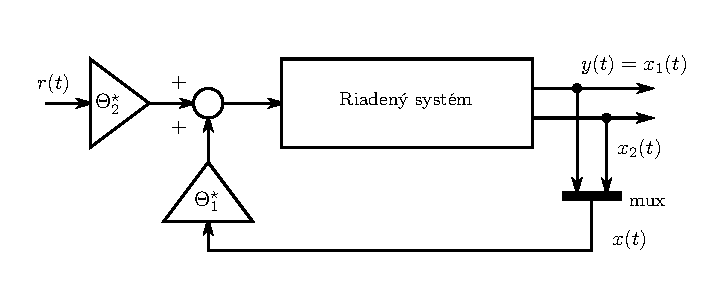
\includegraphics{Obr_41_ZRstavSpVaz_standalone.pdf}
    \caption{Zákon riadenia so stavovou spätnou väzbou -- pôvodný tvar, ktorý je umožnený pre dostupnosť stavového vektora $x(t)$.}
    \label{Obr_41_ZRstavSpVaz}
\end{figure}







V úvode časti uvedený ideálny člen ${\Theta_1^\star}^\naT(t) x(t)$ je teda možné parametrizovať nasledovne. Stavový vektor $x(t)$ je nahradený odhadom $\hat{x}(t) = \begin{bmatrix} y(t) & \hat{x}_2(t) \end{bmatrix}^\naT$, a tiež sa rozdelí $\Theta_1^\star(t) = \begin{bmatrix} k_y^\star & {k_2^\star}^\naT \end{bmatrix}^\naT$, pričom $k_y^\star \in \mathbb{R}$, potom
\begin{equation} \label{n1param}
	\begin{split}
		{\Theta_1^\star}^\naT(t) \hat{x}(t)
		= &
		k_y^\star y(t) + {k_2^\star}^\naT \hat{x}_2(t)
		\\ = &
		k_y^\star y(t)
		+
		{k_2^\star}^\naT
		\text{diag}(g_u) \left[ \frac{\alpha(s)}{\Lambda(s)} \right] u(t)
		+
		{k_2^\star}^\naT
		\text{diag}(g_y) \left[ \frac{\alpha(s)}{\Lambda(s)} \right] y(t)
		+ {k_2^\star}^\naT L y(t)
	\end{split}
\end{equation}










V tomto bode text sa pre jednoduchosť a lepšiu názornosť zavedie úplne nové označovanie, ktorým sa mení označenie niektorých parametrov zákona riadenia, a teda význam pôvodného označovania. Pôvodný ideálny člen formálne zodpovedá výrazu ${\overline{\Theta}_1^\star}^\naT \hat{x}(t)$ a nové označovanie vyplýva zo zapísania rovnice \eqref{n1param} v tvare
\begin{equation} \label{n1param2}
	{\overline{\Theta}_1^\star}^\naT \hat{x}(t)
	=
	{\Theta_1^\star}^\naT \left[ \frac{\alpha(s)}{\Lambda(s)} \right] u(t)
	+
	{\Theta_2^\star}^\naT \left[ \frac{\alpha(s)}{\Lambda(s)} \right] y(t)
	+
	\Theta_3^\star y(t)
\end{equation}
kde sa vzhľadom na \eqref{n1param} zaviedlo označenie ${\Theta_1^\star}^\naT = {k_2^\star}^\naT \text{diag}(g_u)$,   ${\Theta_2^\star}^\naT = {k_2^\star}^\naT \text{diag}(g_y)$ a~$\Theta_3^\star = k_y^\star + {k_2^\star}^\naT L$.

Z uvedeného vyplýva, že ideálny stavový zákon riadenia použitý v predchádzajúcich častiach je možné re-parametrizovať do tvaru
\begin{equation} \label{n1reparamzr}
	u(t)
	=
	{\Theta_1^\star}^\naT \left[ \frac{\alpha(s)}{\Lambda(s)} \right] u(t)
	+
	{\Theta_2^\star}^\naT \left[ \frac{\alpha(s)}{\Lambda(s)} \right] y(t)
	+
	\Theta_3^\star y(t)
	+
	\Theta_4^\star r(t)
\end{equation}








\begin{figure}[t]
    \centering
    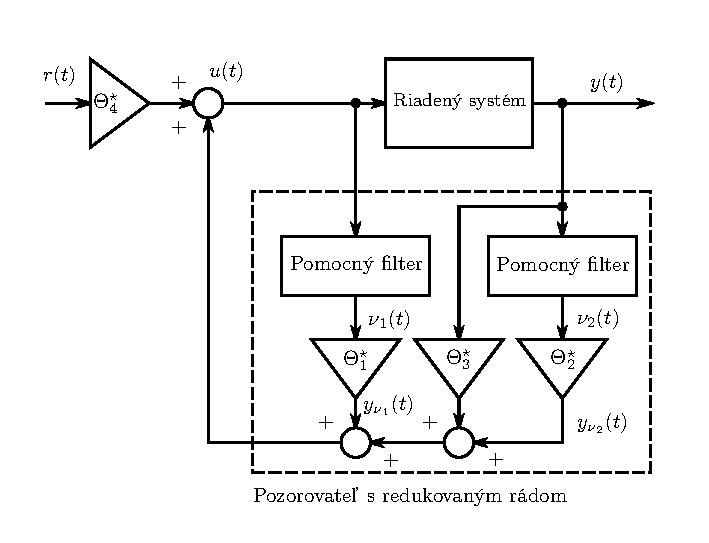
\includegraphics{Obr_PozRedRad_standalone.pdf}
    \caption{Pozorovateľ s redukovaným rádom.}
    \label{Obr_PozRedRad}
\end{figure}











V prvých dvoch členoch zákona riadenia \eqref{n1reparamzr} sú použité takzvané pomocné filtre. Tieto generujú pomocné signály $\nu_1(t)$ a $\nu_2(t)$ upresnené nižšie. Napríklad prvý člen pravej strany v rovnici \eqref{n1reparamzr} možno zapísať v tvare
\begin{equation}
	y_{\nu_1}(t) = {\Theta_1^\star}^\naT \left[\frac{\alpha(s)}{\Lambda(s)}\right] u(t)
	=
	\frac{
	\Theta_{1(n-2)}^\star s^{n-2}    + \cdots + \Theta_{11}^\star s + \Theta_{10}^\star
	}{
	s^{n-1}+ \lambda_{n-2} s^{n-2} + \cdots + \lambda_1 s + \lambda_0
	}
	u(t)
\end{equation}
kde $ \Theta_1^\star = \begin{bmatrix} \Theta_{1(n-2)}^\star  & \cdots & \Theta_{11}^\star & \Theta_{10}^\star \end{bmatrix}^\naT $, alebo v stavovom priestore v tvare \eqref{stavPriestPrvzPomFiltMRCp} na strane \pageref{stavPriestPrvzPomFiltMRCp}. Po označení jednotlivých vektorov a matíc v \eqref{stavPriestPrvzPomFiltMRCp} je prvý pomocný filter v~tvare
\begin{subequations}
	\begin{align}
		\dot \nu_1(t)
		&=
		\Lambda
		\nu_1(t)
		+
		q
		u(t)
		\\
		y_{\nu_1}(t)
		&=
		{\Theta_1^\star}^\naT
		\nu_1(t)
	\end{align}
\end{subequations}



Z uvedeného plynie, že prvý pomocný filter má v~stavovom priestore tvar $ \dot \nu_1(t) = \Lambda \nu_1(t) + q u(t) $, kde $\nu_1$(t) je vektor pomocných signálov generovaných prvým pomocným filtrom (stavový vektor prvého pomocného filtra). Tento je násobený parametrami zákona riadenia ${\Theta_1^\star}^\naT$. Analogicky, druhý prídavný filter má v stavovom priestore tvar $ \dot{\nu}_2(t) = \Lambda \nu_2(t) + q y(t) $. Zákon riadenia využívajúci len vstupno-výstupné signály riadeného systému je potom v tvare
\begin{align} \label{zakriadspoz}
	u(t) = {\Theta_1^\star}^\naT \nu_1(t) + {\Theta_2^\star}^\naT \nu_2(t) + \Theta_3^\star y(t) + \Theta_4^\star r(t)
\end{align}


















\subsection{Formulácia problému riadenia s referenčným modelom}
\label{MRC problém}



Riešením MRC (Model Reference Control -- Riadenie s~referenčným modelom) problému je taký zákon riadenia $u$, ktorý zabezpečí, že výstup sústavy $y$~sleduje výstup referenčného modelu $y_m$~pri danom referenčnom signály $r$.



Uvažujme sústavu opísanú prenosovou funkciou v~tvare
\begin{equation} \label{PFsustavy_MRCp}
	\frac{y(s)}{u(s)} = k_p \frac{Z_p(s)}{R_p(s)}
\end{equation}
kde $Z_p(s)$ je monický, hurwitzov polynóm stupňa $m$, $R_p(s)$ je monický polynóm stupňa $n$ a~$k_p$~je tzv. \emph{vysokofrekvenčné zosilnenie sústavy}. \emph{Relatívny stupeň} sústavy je $n^* = n - m$.

Polynóm sa nazýva \emph{monický} ak je koeficient pri najvyššej mocnine $s$ (v~tomto prípade) rovný jednotke. Polynóm sa nazýva \emph{hurwitzov} ak sú reálne časti všetkých koreňov polynómu záporné.

Nech referenčný model je daný prenosovou funkciou v tvare
\begin{equation} \label{RefModelMRCp}
	\frac{y_m(s)}{r(s)} = W_m(s) = k_m \frac{Z_m(s)}{R_m(s)}
\end{equation}
kde $k_m$ je vysokofrekvenčné zosilnenie referenčného modelu, polynóm $Z_m(s)$ je monický Hurwitzov polynóm stupňa $m_m$, $R_m(s)$ monický Hurwitzov polynóm stupňa $n_m$, pričom relatívny stupeň $n^*_m = n_m - m_m = n^*$.

Zákon riadenia, ktorý rieši MRC problém je nasledovný. Najskôr uvedieme jeho všeobecný zápis, avšak pre lepšiu názornosť budeme riešenie MRC problému vyšetrovať na zjednodušenom konkrétnom príklade. Všeobecný tvar zákona riadenia, ktorý rieši MRC problém je
\begin{equation} \label{generalControlLaw}
    u = {\Theta_1^\star}^\naT \frac{\alpha(s)}{\Lambda(s)} u + {\Theta_2^\star}^\naT \frac{\alpha(s)}{\Lambda(s)} y + \Theta_3^\star y + \Theta_4^\star r
\end{equation}
kde $\alpha(s)$ je vektor obsahujúci mocniny $s$, $\alpha(s) = \begin{bmatrix} s^{n-2}, \ldots,s, 1 \end{bmatrix}^\naT$ ak $n\geq 2$, inak $\alpha(s) = 0$. Vektory $\Theta_1^\star \in \mathbb{R}^{n-1}$, $\Theta_2^\star \in \mathbb{R}^{n-1}$ a skaláry $\Theta_3^\star \in \mathbb{R}^1$, $\Theta_4^\star \in \mathbb{R}^1$ sú konštantné parametre zákona riadenia, ktorých hodnoty hľadáme.  $\Lambda(s)$ je ľubovolný monický Hurwitzov polynóm stupňa $n-1$ obsahujúci $Z_m(s)$ ako faktor
\begin{equation}
	\Lambda(s) = \Lambda_0(s) Z_m(s)
\end{equation}
a teda aj $\Lambda_0(s)$ je ľubovolný monický Hurwitzov polynóm zodpovedajúceho stupňa.

















\subsubsection{Ilustrácia na príklade systému 2. rádu}
\label{MRCproblemPriklad}



Uvažujme systém opísaný prenosovou funkciou v tvare
\begin{equation} \label{genaralFormOfPlant04}
	y(s) = k_p \frac{s + b_0}{ s^2 + a_1 s + a_0} \, u(s)
\end{equation}
kde $a_i, b_i$ sú konštanty ($b_0 > 0$). Referenčný model zvoľme tak aby mal rovnaký relatívny stupeň ako sústava.
\begin{equation}
	y_m(s) = W_m(s)r(s) = k_m \frac{s + b_{0m}}{ s^2 + a_{1m} s + a_{0m}} r(s)
\end{equation}

V tomto konkrétnom príklade, zákon riadenia, ktorý rieši MRC problém je v tvare
\begin{equation} \label{controlLaw}
	u(s) = \Theta_1^\star \frac{1}{(s + \lambda)} u(s) + \Theta_2^\star \frac{1}{(s + \lambda)} y(s) + \Theta_3^\star y(s) + \Theta_4^\star r(s)
\end{equation}
kde sme použili $\alpha(s) = 1$ a $\Lambda(s) = (s + \lambda)$. V tomto prípade $\Theta_1^\star$, $\Theta_2^\star$ aj $\Theta_3^\star$ a $\Theta_4^\star$ sú skalárne konštanty -- parametre zákona riadenia.
Zákon riadenia \eqref{controlLaw} možno upraviť do tvaru
\begin{subequations}
	\begin{align}
		\left( 1 - \frac{ \Theta_1^\star }{ (s + \lambda)} \right) u(s)
		&=
		\left( \frac{ \Theta_2^\star }{ (s + \lambda)} + \Theta_3^\star \right) y(s) + \Theta_4^\star r(s)
		\\
        \left( \frac{ (s + \lambda) - \Theta_1^\star }{ (s + \lambda)} \right) u(s)
		& =
		\left( \frac{ \Theta_2^\star + \Theta_3^\star (s + \lambda) }{ (s + \lambda)} \right) y(s) + \Theta_4^\star r(s)
		\\
		\label{controlLaw04_2}
		u(s) &= \frac{\Theta_2^\star + \Theta_3^\star (s + \lambda)}{(s + \lambda) - \Theta_1^\star} y(s) + \frac{ \Theta_4^\star (s + \lambda)}{(s + \lambda) - \Theta_1^\star} r(s)
	\end{align}
\end{subequations}






Dosadením \eqref{controlLaw04_2} do \eqref{genaralFormOfPlant04} získame prenosovú funkciu URO v tvare \eqref{MRCRovniceNavrchuStrany}:
\begin{subequations} \label{MRCRovniceNavrchuStrany}
	\begin{align}
		\begin{split}
		\label{genaralFormOfCL}
			y(s)
			=
			k_p
			\frac{
				s + b_0
				}{
				s^2 + a_1 s + a_0}
			\,
			\left(
				\frac{
					\Theta_2^\star
					+
					\Theta_3^\star
					(s + \lambda)
					}{
					(s + \lambda)
					-
					\Theta_1^\star}
				y(s)
				+
				\frac{
					\Theta_4^\star
					(s + \lambda)
					}{
					(s + \lambda)
					-
					\Theta_1^\star}
				r(s)
			\right)
		\end{split}
		\\
		\begin{split}
		\left(
			1
			-
			\frac{
				k_p
				(s + b_0)
				\left(
					\Theta_2^\star
					+
					\Theta_3^\star
					(s + \lambda)
				\right)
				}{
				(s^2 + a_1 s + a_0)
				\left(
					(s + \lambda)
					-
					\Theta_1^\star
				\right)}
		\right)
			y(s)
			=
			\frac{
				k_p
				(s + b_0)
				\Theta_4^\star
				(s + \lambda)
				}{
				(s^2 + a_1 s + a_0)
				\left(
					(s + \lambda)
					-
					\Theta_1^\star
				\right)}
			r(s)
		\end{split}
		\\
		\begin{split}
		\left(
			\frac{
				(s^2 + a_1 s + a_0)
				\left(
					(s + \lambda)
					-
					\Theta_1^\star
				\right)
				-
				k_p
				(s + b_0)
				\left(
					\Theta_2^\star
					+
					\Theta_3^\star
					(s + \lambda)
				\right)
				}{
				(s^2 + a_1 s + a_0)
				\left(
					(s + \lambda)
					-
					\Theta_1^\star
				\right)}
		\right)
			y(s)
			=\\=
			\frac{
				k_p
				(s + b_0)
				\Theta_4^\star
				(s + \lambda)
				}{
				(s^2 + a_1 s + a_0)
				\left(
					(s + \lambda)
					-
					\Theta_1^\star
				\right)}
				r(s)
		\end{split}
		\\
		\label{genaralFormOfCL_04}
		\begin{split}
			\frac{y(s)}{r(s)}
			=
			\frac{
				k_p
				(s + b_0)
				\Theta_4^\star
				(s + \lambda)
				}{
				(s^2 + a_1 s + a_0)
				\left(
					(s + \lambda)
					-
					\Theta_1^\star
				\right)
				-
				k_p
				(s + b_0)
				\left(
					\Theta_2^\star
					+
					\Theta_3^\star
					(s + \lambda)
				\right)}
		\end{split}
	\end{align}
\end{subequations}









Prenosovú funkciu \eqref{genaralFormOfCL_04} označme $G_c(s)$. Výstupná veličina sústavy bude sledovať výstupnú veličinu referenčného modelu ak $G_c(s) = W_m(s)$. Táto podmienka bude splnená ak
\begin{align}
	\Theta_4^\star &= \frac{k_m}{k_p} \label{idealTheta4} \\
	(s + \lambda) &= \Lambda_0(s) (s + b_{0m}) = (s + b_{0m}) \label{lambda}
\end{align}
pričom \eqref{idealTheta4} je prvou podmienkou zhody, \eqref{lambda} je voľbou polynómu $\Lambda(s)$ stupňa $n-1$ kde v tomto prípade $\Lambda_0(s) = 1$ a teda $\lambda = b_{0m}$ a druhou podmienkou zhody je
\begin{equation} \label{matchingEquation}
    \begin{split}
    	&(s^2 + a_1 s + a_0)
    	\left( (s + \lambda) - \Theta_1^\star \right)
    	-
    	k_p
    	(s + b_0)
    	\left( \Theta_2^\star + \Theta_3^\star (s + \lambda) \right)
    	\\&=
    	(s + b_0)   ( s^2 + a_{1m} s + a_{0m})
    \end{split}
\end{equation}
Potom možno \eqref{genaralFormOfCL_04} zapísať v tvare
\begin{equation} \label{genaralFormOfCL_05}
	\frac{y(s)}{r(s)}
	=
	\frac{
		k_p
		(s + b_0)
		\frac{k_m}{k_p}
		(s + b_{0m})
		}{
		(s + b_0)
		( s^2 + a_{1m} s + a_{0m})}
	=
	\frac{
		k_m
		(s + b_{0m})
		}{
		( s^2 + a_{1m} s + a_{0m})}
	=
	W_m(s)
\end{equation}
V prenosovej funkcii \eqref{genaralFormOfCL_05} dochádza ku vzájomnému  vykráteniu sa polynómu $(s + b_0)$. Táto operácia je možná, pretože tieto polynómy majú korene v zápornej polrovice komplexnej roviny a teda sú stabilné (Hurwitzove). Taký je predpoklad pre $Z_p(s)$. Polynómy, ktoré nie sú Hurwitzove nemožno v prenosovej funkcii navzájom vykrátiť. Podmienku zhody \eqref{matchingEquation} je možné zapísať aj v maticovom tvare porovnaním koeficientov pri rovnakých mocninách na oboch stranách
\begin{equation} \label{idealParameters}
	\begin{bmatrix}
		-1 & 0 & -k_p \\
		-a_1 & -k_p & -(k_p b_{0m} + k_p b_0) \\
		-a_0 & -k_p b_0 & -k_p b_0 b_{0m}
	\end{bmatrix}
	\begin{bmatrix}
    	  \Theta_1^\star \\
		  \Theta_2^\star \\
		  \Theta_3^\star
 	\end{bmatrix}
	=
	\begin{bmatrix}
    	a_{1m} + b_0 - b_{0m} - a_1 \\
    	a_{0m} + b_0 a_{1m} - a_1 b_{0m} - a_0 \\
    	b_0 a_{0m} - a_0 b_{0m}
  	\end{bmatrix}
\end{equation}
čo je sústava algebraických rovníc v tvare $M_s \Theta_s = p_s$ a~teda existencia takého vektora $\Theta_s$, ktorý spĺňa rovnosť, je závislá od vlastností matice $M_s$. Z~podmienok zhody \eqref{idealTheta4} a~\eqref{idealParameters} plynú konkrétne hodnoty parametrov zákona riadenia, ktoré riešia daný MRC problém.

Predchchádzajúci postup je možné zapísať prehladnejšie (pre prehľadnosť vynecháme aj zátvorky s laplaceovou premennou $(s)$):

Zákon riadenia
\begin{subequations}
	\begin{align}
		u
		&=
		\frac{\Theta_1^\star}{\Lambda}
		u
		+
		\frac{\Theta_2^\star}{\Lambda}
		y
		+
		\Theta_3^\star
		y
		+
		\Theta_4^\star
		r
		\\
		\left(
			1
			-
			\frac{\Theta_1^\star}{\Lambda}
		\right)
		u
		&=
		\left(
			\frac{\Theta_2^\star}{\Lambda}
			+
			\Theta_3^\star
		\right)
		y
		+
		\Theta_4^\star
		r
		\\
		\frac{\Lambda - \Theta_1^\star}{\Lambda}
		u
		&=
		\frac{
			\Theta_2^\star
			+
			\Theta_3^\star\Lambda
			}{
			\Lambda}
		y
		+
		\Theta_4^\star
		r
		\\
		u
		&=
		\frac{
			\Theta_2^\star
			+
			\Theta_3^\star\Lambda
			}{
			\Lambda - \Theta_1^\star}
		y
		+
		\frac{
		\Theta_4^\star \Lambda
		}{
		\Lambda - \Theta_1^\star}
		r
	\end{align}
\end{subequations}

Uzavretý regulačný obvod
\begin{subequations}
	\begin{align}
		y
		&=
		k_p
		\frac{Z_p}{R_p}
		\left(
				\frac{
			\Theta_2^\star
			+
			\Theta_3^\star\Lambda
			}{
			\Lambda - \Theta_1^\star}
		y
		+
		\frac{
		\Theta_4^\star \Lambda
		}{
		\Lambda - \Theta_1^\star}
		r
		\right)
\\
		\left(
			1
			-
			\frac{
				k_p
				Z_p
				\left(
					\Theta_2^\star
					+
					\Theta_3^\star\Lambda
				\right)
				}{
				R_p
				\left(
					\Lambda - \Theta_1^\star
				\right)}
		\right)
		y
		&=
		\frac{
			k_p
			Z_p
			\Theta_4^\star
			\Lambda
			}{
			R_p
			\left(
				\Lambda - \Theta_1^\star
			\right)}
		r
\\
		\frac{
			R_p
			\left(
				\Lambda - \Theta_1^\star
			\right)
			-
			k_p
			Z_p
			\left(
				\Theta_2^\star
				+
				\Theta_3^\star\Lambda
			\right)
			}{
			R_p
			\left(
				\Lambda - \Theta_1^\star
			\right)}
		y
		&=
		\frac{
			k_p
			Z_p
			\Theta_4^\star
			\Lambda
			}{
			R_p
			\left(
				\Lambda - \Theta_1^\star
			\right)}
		r
\\
		y
		&=
		\frac{
			k_p
			Z_p
			\Theta_4^\star
			\Lambda
			}{
			R_p
			\left(
				\Lambda - \Theta_1^\star
			\right)
			-
			k_p
			Z_p
			\left(
				\Theta_2^\star
				+
				\Theta_3^\star\Lambda
			\right)}
		r
	\end{align}
\end{subequations}

Podmienky zhody
\begin{subequations}
	\begin{align}
		\Theta_4^\star &= \frac{k_m}{k_p} \label{idealTheta4_02} \\
		\Lambda &= Z_m  \label{lambda_02}\\
		R_p \left( \Lambda - \Theta_1^\star \right) - k_p Z_p \left( \Theta_2^\star + \Theta_3^\star\Lambda \right)
		&=
		Z_p R_m
	\end{align}
\end{subequations}


















\subsubsection{Zovšeobecnenie pre systém $n$. rádu}


Pri uvažovaní všeobecného zákona riadena v tvare \eqref{generalControlLaw} má prenosová funkcia uzavretého regulačného obvodu tvar
\begin{equation}
	y
	=
	\frac{
		k_p
		Z_p
		\Theta_4^\star
		\Lambda^2
		}{
		\Lambda
		\left(
			R_p
			\left(
				\Lambda - {\Theta_1^\star}^\naT	\alpha(s)
			\right)
			-
			k_p
			Z_p
			\left(
				{\Theta_2^\star}^\naT	\alpha(s)
				+
				\Theta_3^\star \Lambda
			\right)
		\right)}
	r
\end{equation}
a podmienky zhody
\begin{subequations}
	\begin{align}
		\Theta_4^\star &= \frac{k_m}{k_p} \label{idealTheta4_03} \\
		\Lambda &= \Lambda_0 Z_m \label{lambda_03} \\
		R_p
		\left(
			\Lambda - {\Theta_1^\star}^\naT \alpha(s)
		\right)
		-
		k_p
		Z_p
		\left(
			{\Theta_2^\star}^\naT \alpha(s)
			+
			\Theta_3^\star \Lambda
		\right)
	    &=
	    Z_p
	    \Lambda_0
	    R_m
	\end{align}
\end{subequations}

Predpoklady pri, ktorých sú tieto podmienky splniteľné sú intuitívne zrejmé z~predchádzajúceho príkladu v časti \ref{MRCproblemPriklad}. Hlbšou analýzou MRC problému sa v~tomto kurze zaoberať nebudeme. Poslucháča odkazujeme na odporúčanú literatúru, kde nájde všetky potrebné (matematické) detaily k riešeniu MRC problému.

































\subsection{Teoretický opis výsledného URO v stavovom priestore}




V tejto časti vyjadríme uzavretý regulačný obvod, ktorý vznikne riešením MRC problému, pomocou opisu v~stavovom priestore.



\subsubsection{Ilustrácia na príklade systému 2. rádu}

Opäť začneme zjednodušeným príkladom \ref{MRCproblemPriklad}, a~v~ďalšej časti dodáme pre úplnosť všeobecný zápis URO v~stavovom priestore.

Sústava v tvare \eqref{PFsustavy_MRCp}, konkrétne \eqref{genaralFormOfPlant04}, môže byť reprezentovaná opisom v~stavovom priestore v tvare
\begin{subequations}
	\begin{align}
		 \dot x &= A x + b u \\
		 y &= c^\naT x
	\end{align}
\end{subequations}
kde $x$ je vektor stavových veličín sústavy a $A$; $b$; $c^\naT$ sú konštantné matice (vektory) zodpovedajúcich rozmerov. V tomto prípade nekladieme žiadne podmienky na formu (kanonickú) matice $A$, ako to bolo v prípade stavového MRAC-u.

Uvažujeme zákon riadenia \eqref{controlLaw}, pripomeňme:
\begin{equation} \label{ZakonRiadeniaMRCp}
	u(s) = \Theta_1^\star \frac{1}{(s + \lambda)} u(s) + \Theta_2^\star \frac{1}{(s + \lambda)} y(s) + \Theta_3^\star y(s) + \Theta_4^\star r(s)
\end{equation}
V prvých dvoch členoch zákona riadenia \eqref{ZakonRiadeniaMRCp} sú použité takzvané prídavné filtre, ktorých vstupom je buď akčný zásah $u$ (vstupný signál sústavy) alebo výstupná (riadená) veličina $y$. Tieto prídavné filtre sú tiež nazývané pomocné, či prídavné generátory, generujú prídavné (pomocné) signály. Oba prídavné filtre sú rovnaké, v~ tomto prípade dané prenosovou funkciou $\frac{1}{(s + \lambda)}$. Výstupné signály filtrov sú v~tomto prípade skalárne signály. Vo všeobecnosti sú výstupné signály pomocných filtrov vektory signálov s~rovnakým rozmerom ako vektory parametrov $\Theta_1^\star$ a~$\Theta_2^\star$, viď všeobecný zápis zákona riadenia \eqref{generalControlLaw}. Označme výstupné signály prídavných filtrov $\nu_1$ a~$\nu_2$. Tieto signály sa násobia parametrami zákona riadenia ${{\Theta}_1^\star}$ a ${{\Theta}_2^\star}$. Prídané filtre možno zapísať v tvare
\begin{subequations}
	\begin{align}
		 \dot \nu_1 &= -\lambda \nu_1 + u \\
		 \dot \nu_2 &= -\lambda \nu_2 + y = -\lambda \nu_2 + c^\naT x
	\end{align}
\end{subequations}

Jednoduchým pridaním týchto pomocných signálov k sústave máme sústavu rovníc:
\begin{subequations} \label{DoplnenaSustavaMRCp}
	\begin{align}
		 \dot x &= A x + b u \\
		 \dot \nu_1 &= -\lambda \nu_1 + u \\
		 \dot \nu_2 &= -\lambda \nu_2 + c^\naT x \\
		 y &= c^\naT x
	\end{align}
\end{subequations}
Sústavu rovníc \eqref{DoplnenaSustavaMRCp} budeme nazývať \emph{doplnená sústava}. Doplnenú sústavu \eqref{DoplnenaSustavaMRCp} možno zapísať v maticovom tvare
\begin{subequations}
	\begin{align}
		\begin{bmatrix} \dot x \\ \dot{\nu}_1 \\ \dot{\nu}_2 \end{bmatrix}
		&=
		\begin{bmatrix} A & 0 & 0 \\ 0 & -\lambda & 0 \\ c^\naT & 0 & -\lambda \end{bmatrix}
	 	\begin{bmatrix} x \\ \nu_1 \\ \nu_2 \end{bmatrix}
		+
		\begin{bmatrix} b \\ 1\\ 0 \end{bmatrix}
	 	u
	 	\\
	 	y &= \begin{bmatrix} c^\naT & 0 & 0 \end{bmatrix}
	 	\begin{bmatrix} x \\ \nu_1 \\ \nu_2 \end{bmatrix}
	\end{align}
\end{subequations}
a po označení jednotlivých matíc a vektorov
\begin{subequations}
\label{augmentedPlant}
	\begin{align}
		 \dot X &= A_o X + B_c u \\
		 y &= C_c^\naT X \label{outputOfAugmentedPlant}
	\end{align}
\end{subequations}

Zákon riadenia \eqref{ZakonRiadeniaMRCp} zapíšeme v takom vektorovom tvare, v ktorom je možné využiť stavový vektor doplnenej sústavy $X$:
\begin{equation} \label{ZakonRiadeniaMaticMRCp}
	u = {\Theta_c^\star}^\naT D X + \Theta_4^\star r
\end{equation}
kde $ \Theta_c^\star = \begin{bmatrix} \Theta_3^\star & \Theta_1^\star & \Theta_2^\star \end{bmatrix}^\naT $; $\Theta_4^\star$ sú parametre zákona riadenia a maticu
\begin{align*}
	D = \begin{bmatrix} c^\naT & 0 & 0 \\ 0 & 1 & 0 \\ 0 & 0 & 1 \end{bmatrix}
\end{align*}
sme zaviedli práve preto aby sme v zákone riadenia \eqref{ZakonRiadeniaMaticMRCp} mohli priamo písať stavový vektor $X$. Tvar, v ktorom sa zákon riadenia \eqref{ZakonRiadeniaMaticMRCp} viac podobá na pôvodný zápis \eqref{ZakonRiadeniaMRCp}, a ktorý vyplíva priamo z \eqref{ZakonRiadeniaMaticMRCp} je
\begin{subequations} \label{ZakonRiadeniaMaticMRCp_02}
	\begin{align}
		u &= \Theta_1^\star \nu_1 + \Theta_2^\star \nu_2 + \Theta_3^\star {c}^\naT x + \Theta_4^\star r \\
		u &= \Theta_1^\star \nu_1 + \Theta_2^\star \nu_2 + \Theta_3^\star y + \Theta_4^\star r
	\end{align}
\end{subequations}








Dosadením \eqref{ZakonRiadeniaMaticMRCp} do \eqref{augmentedPlant} získame opis URO v~stavovom priestore v tvare (výstupnú rovnicu vynechávame, pretože sa nemení)
\begin{subequations} \label{UROaugmentedPlant}
	\begin{align}
		\dot X &= A_o X + B_c \left( {\Theta_c^\star}^\naT D X + \Theta_4^\star r \right) \\
		\dot X &= A_o X + B_c {\Theta_c^\star}^\naT D X + B_c \Theta_4^\star r \\
		\dot X &= \left( A_o + B_c {\Theta_c^\star}^\naT D \right) X + B_c \Theta_4^\star r \\
		\dot X &= A_c X + B_c \Theta_4^\star r
	\end{align}
\end{subequations}
kde
\begin{equation}
	\begin{split}
		A_c &= A_o + B_c {\Theta_c^\star}^\naT D \\
		&=
		\begin{bmatrix} A & 0 & 0 \\ 0 & -\lambda & 0 \\ c^\naT & 0 & -\lambda \end{bmatrix}
	 	+
	 	\begin{bmatrix} b \\ 1\\ 0 \end{bmatrix}
	 	\begin{bmatrix} \Theta_3^\star & \Theta_1^\star & \Theta_2^\star \end{bmatrix}
		\begin{bmatrix} c^\naT & 0 & 0 \\ 0 & 1 & 0 \\ 0 & 0 & 1 \end{bmatrix}
		\\
		&=
		\begin{bmatrix} A & 0 & 0 \\ 0 & -\lambda & 0 \\ c^\naT & 0 & -\lambda \end{bmatrix}
	 	+
	 	\begin{bmatrix} b \Theta_3^\star & b \Theta_1^\star & b \Theta_2^\star \\ \Theta_3^\star & \Theta_1^\star & \Theta_2^\star \\ 0 & 0 & 0 \end{bmatrix}
		\begin{bmatrix} c^\naT  & 0 & 0 \\ 0 & 1 & 0 \\ 0 & 0 & 1 \end{bmatrix}
		\\
		&=
		\begin{bmatrix} A & 0 & 0 \\ 0 & -\lambda & 0 \\ c^\naT & 0 & -\lambda \end{bmatrix}
	 	+
	 	\begin{bmatrix} b \Theta_3^\star c^\naT & b \Theta_1^\star & b \Theta_2^\star \\ \Theta_3^\star c^\naT & \Theta_1^\star & \Theta_2^\star \\ 0 & 0 & 0 \end{bmatrix}
		\\
		& =
		\begin{bmatrix} A +  b \Theta_3^\star c^\naT & b \Theta_1^\star & b \Theta_2^\star \\ \Theta_3^\star c^\naT & -\lambda + \Theta_1^\star & \Theta_2^\star \\ c^\naT & 0 & -\lambda \end{bmatrix}
	\end{split}
\end{equation}

Pretože uzavretý regulačný obvod zapísaný v tvare
\begin{subequations} \label{UROaugmentedPlant_02}
	\begin{align}
		\dot X &= A_c X + B_c \Theta_4^\star r \\
		y &= C_c^\naT X
	\end{align}
\end{subequations}
obsahuje ideálne parametre zákona riadenia, teda také, ktoré spĺňajú podmienky zhody musí sa tento zhodovať s referenčným modelom. Preto tzv. \emph{neminimálna reprezentácia} prenosovej funkcie referenčného modelu \eqref{RefModelMRCp} v stavovom priestore je
\begin{subequations} \label{NeminimalRMMRCp}
	\begin{align}
		\dot X_m &= A_c X_m + B_c \Theta_4^\star r \\
		y_m &= C_c^\naT X_m
	\end{align}
\end{subequations}
kde $X_m$ sú stavové veličiny neminimálnej reprezentácie modelu










\subsubsection{Zovšeobecnenie pre systém $n$. rádu}




Uvažujeme zákon riadenia \eqref{generalControlLaw}, pripomeňme:
\begin{equation} \label{generalControlLaw_02}
	u = {\Theta_1^\star}^\naT \frac{\alpha(s)}{\Lambda(s)} u + {\Theta_2^\star}^\naT \frac{\alpha(s)}{\Lambda(s)} y + \Theta_3^\star y + \Theta_4^\star r
\end{equation}
kde $\alpha(s)$ je vektor obsahujúci mocniny $s$, $\alpha(s) = \begin{bmatrix} s^{n-2}, \ldots, s, 1 \end{bmatrix}^\naT$ ak $n\geq 2$, inak $\alpha(s) = 0$. Vektory ${\Theta_1^\star}, \Theta_2^\star \in \mathbb{R}^{n-1}$ a skaláry $\Theta_3^\star, \Theta_4^\star \in \mathbb{R}^1$ sú konštantné parametre zákona riadenia. $\Lambda(s)$ je ľubovolný monický Hurwitzov polynóm stupňa $n-1$.

Napríklad prvý člen v \eqref{generalControlLaw_02} možno zapísať v tvare
\begin{equation}
	y_{\nu_1} = {\Theta_1^\star}^\naT \frac{\alpha(s)}{\Lambda(s)} u
    =
	\frac{
	\Theta_{1(n-2)}^\star s^{n-2}    + \cdots + \Theta_{11}^\star s + \Theta_{10}^\star
	}{
	s^{n-1}+ \lambda_{n-2} s^{n-2} + \cdots + \lambda_1 s + \lambda_0
	}
	u
\end{equation}
kde $ \Theta_1^\star = \begin{bmatrix} \Theta_{1(n-2)}^\star  & \cdots & \Theta_{11}^\star & \Theta_{10}^\star \end{bmatrix}^\naT $, alebo v stavovom priestore v tvare
\begin{subequations} \label{stavPriestPrvzPomFiltMRCp}
	\begin{align}
		\begin{bmatrix}
			\dot{\nu}_{1(n-2)} \\
			\dot{\nu}_{1(n-3)} \\
			\dot{\nu}_{1(n-4)} \\
			\vdots \\
			\dot{\nu}_{10}
		\end{bmatrix}
		&=
		\begin{bmatrix}
			-\lambda_{n-2} & -\lambda_{n-3} &  \cdots & -\lambda_2 & -\lambda_1 & -\lambda_0\\
			1 & 0 &  \cdots & 0 & 0 & 0  \\
			0 & 1 & \ddots & 0 & 0 & 0 \\
			\vdots & \ddots & \ddots & \ddots & \vdots & \vdots \\
			0 & 0 & \ddots & 1 &  0 & 0 \\
			0 & 0 & \cdots & 0 &  1 & 0
		\end{bmatrix}
		\begin{bmatrix}
			\nu_{1(n-2)} \\
			\nu_{1(n-3)} \\
			\nu_{1(n-4)} \\
			\vdots \\
			\nu_{10}
		\end{bmatrix}
		+
		\begin{bmatrix}
			1 \\
			0 \\
			0 \\
			\vdots \\
			0
		\end{bmatrix}
		u
		\\
		y_{\nu_1}
		&=
		\begin{bmatrix}
			\Theta_{1(n-2)}^\star  &
			\Theta_{1(n-3)}^\star  &
			\Theta_{1(n-4)}^\star  &
			\cdots &
			\Theta_{10}^\star
		\end{bmatrix}
		\begin{bmatrix}
			\nu_{1(n-2)} \\
			\nu_{1(n-3)} \\
			\nu_{1(n-4)} \\
			\vdots \\
			\nu_{10}
		\end{bmatrix}
	\end{align}
\end{subequations}
Označme v \eqref{stavPriestPrvzPomFiltMRCp} jednotlivé vektory a maticu:
\begin{subequations}
	\begin{align}
		\dot \nu_1 &= \Lambda \nu_1 + q u \\
		y_{\nu_1} &= {\Theta_1^\star}^\naT \nu_1
	\end{align}
\end{subequations}



Z uvedeného vyplýva, že prvý prídavný filter má v~stavovom priestore tvar $\dot \nu_1 = \Lambda \nu_1 + q u $ kde $\nu_1$ je vektor pomocných signálov generovaných prvým pomocným generátorom (stavový vektor prvého pomocného generátora). Tento je násobený parametrami zákona riadenia ${\Theta_1^\star}^\naT$. Analogicky, druhý prídavný filter má v stavovom priestore tvar $\dot \nu_2 = \Lambda \nu_2 + q y = \Lambda \nu_2 + q c^\naT x$.
Doplnená sústava vo všeobecnom tvare je
\begin{subequations} \label{vsDoplnenaSustavaMRCp}
	\begin{align}
		\dot x &= A x + b u \\
		\dot \nu_1 &= \Lambda \nu_1 + q u \\
		\dot \nu_2 &= \Lambda \nu_2 + q c^\naT x \\
		 y &= c^\naT x
	\end{align}
\end{subequations}
Potom v \eqref{augmentedPlant} sú
\begin{align} \label{vsMaticeDoplnenejSustMRCp}
 	x = \begin{bmatrix} x \\ \nu_1 \\ \nu_2 \end{bmatrix}   ; \quad
	A_0 = \begin{bmatrix} A & 0 & 0 \\ 0 & \Lambda & 0 \\ q c^\naT & 0 & \Lambda \end{bmatrix}   ; \quad
	b_c = \begin{bmatrix} b \\ q\\ 0 \end{bmatrix}   ; \quad
    c_c^\naT = \begin{bmatrix} c^\naT & 0 & 0 \end{bmatrix}
\end{align}

Zákon riadenia \eqref{generalControlLaw_02} zapíšeme vo vektorovom tvare:
\begin{equation} \label{vsZakonRiadeniaMaticMRCp}
	u = {\Theta_c^\star}^\naT D x + \Theta_4^\star r
\end{equation}
kde $ \Theta_c^\star = \begin{bmatrix} \Theta_3^\star & {\Theta_1^\star}^\naT & {\Theta_2^\star}^\naT \end{bmatrix}^\naT; \; \Theta_4^\star $ sú parametre zákona riadenia a maticu
\begin{align*}
	D = \begin{bmatrix} c^\naT & 0 & 0 \\ 0 & I & 0 \\ 0 & 0 & I \end{bmatrix}
\end{align*}
sme zaviedli práve preto aby sme v zákone riadenia \eqref{vsZakonRiadeniaMaticMRCp} mohli priamo písať stavový vektor $x$. Tvar, v ktorom sa zákon riadenia \eqref{vsZakonRiadeniaMaticMRCp} viac podobá na pôvodný zápis \eqref{generalControlLaw_02}, a ktorý vyplíva priamo z \eqref{vsZakonRiadeniaMaticMRCp} je
\begin{subequations} \label{vsZakonRiadeniaMaticMRCp_02}
	\begin{align}
		u &= {\Theta_1^\star}^\naT \nu_1 + {\Theta_2^\star}^\naT \nu_2 + \Theta_3^\star {c}^\naT x + \Theta_4^\star r \\
		u &= {\Theta_1^\star}^\naT \nu_1 + {\Theta_2^\star}^\naT \nu_2 + \Theta_3^\star y + \Theta_4^\star r
	\end{align}
\end{subequations}

Dosadením \eqref{vsZakonRiadeniaMaticMRCp} do \eqref{augmentedPlant}, v ktorej sú ale matice \eqref{vsMaticeDoplnenejSustMRCp}, získame opis URO v~stavovom priestore v tvare \eqref{UROaugmentedPlant_02}, a~matica
 $A_c$  má tvar
\begin{equation}
	\begin{split}
		A_c &= A_o + b_c {\Theta_c^\star}^\naT D \\
		&=
        \begin{bmatrix}  A & 0 & 0 \\ 0 & \Lambda & 0 \\ q c^\naT & 0 & \Lambda \end{bmatrix}
	 	+
	 	\begin{bmatrix} b \\ q\\ 0 \end{bmatrix}
	 	\begin{bmatrix} \Theta_3^\star & {\Theta_1^\star}^\naT & {\Theta_2^\star}^\naT \end{bmatrix}
		\begin{bmatrix} c^\naT & 0 & 0 \\ 0 & I & 0 \\ 0 & 0 & I \end{bmatrix} \\
		&=
        \begin{bmatrix} A & 0 & 0 \\ 0 & \Lambda & 0 \\ q c^\naT & 0 & \Lambda \end{bmatrix}
	 	+
	 	\begin{bmatrix}
			b \Theta_3^\star & b {\Theta_1^\star}^\naT & b {\Theta_2^\star}^\naT \\
			q \Theta_3^\star & q {\Theta_1^\star}^\naT & q {\Theta_2^\star}^\naT \\
			0 & 0 & 0
		\end{bmatrix}
		\begin{bmatrix} c^\naT  & 0 & 0 \\ 0 & I & 0 \\ 0 & 0 & I \end{bmatrix} \\
		&=
		\begin{bmatrix} A & 0 & 0 \\ 0 & \Lambda & 0 \\ q c^\naT & 0 & \Lambda \end{bmatrix}
	 	+
	 	\begin{bmatrix}
			b \Theta_3^\star c^\naT & b {\Theta_1^\star}^\naT & b {\Theta_2^\star}^\naT \\
			q \Theta_3^\star c^\naT & q {\Theta_1^\star}^\naT & q {\Theta_2^\star}^\naT \\
			0 & 0 & 0
		\end{bmatrix} \\
		&=
		\begin{bmatrix}
             A +  b \Theta_3^\star c^\naT&
	    	 b {\Theta_1^\star}^\naT &
	    	 b {\Theta_2^\star}^\naT \\
	    	 q \Theta_3^\star c^\naT &
	    	 \Lambda + q {\Theta_1^\star}^\naT &
	    	 q {\Theta_2^\star}^\naT \\
	    	 q c^\naT & 0 & \Lambda
	 	\end{bmatrix}
	\end{split}
\end{equation}

Pretože takto všeobecne opísaný URO obsahuje ideálne parametre zákona riadenia, teda také, ktoré spĺňajú podmienky zhody musí sa tento zhodovať so všeobecným referenčným modelom \eqref{RefModelMRCp}, ktorého neminimálna reprezentácia v~stavovom priestore má tvar
\begin{subequations} \label{vsNeminimalRMMRCp}
	\begin{align}
		\dot x_m &= A_c x_m + \overline{b}_c r \\
		y_m &= c_c^\naT x_m
	\end{align}
\end{subequations}
kde $x_m$ sú stavové veličiny neminimálnej reprezentácie referenčného modelu a kde sme označili $\overline{b}_c = b_c \Theta_4^\star$.































\section{Príklad k téme \emph{MRC vo všeobecnosti}}
\label{pkTMRC}



Tento príklad sa týka riadenia s referenčným modelom avšak bez adaptácie. Cieľom tu teda nie je návrh adaptívneho riadiaceho systému. Cieľom je oboznámenie sa s riešením MRC problému (problému návrhu (výpočtu) riadenia s referenčným modelom). Tu uvedené zároveň slúži na priebežné zopakovanie vybraných tém súvisiacich s numerickou simuláciou.







\subsection{Úlohy}


\begin{enumerate}[leftmargin=0pt, labelsep=4mm, itemsep=0pt]

    \item Uvažujme riadený systém\footnote{Uvedený riadený systém je prevzatý z článku publikovanom v prestížnom elektronickom časopise posterus.sk (nemýliť si so Slniečkom, už nevychádza), viď \cite{Tar11}.}, ktorý pracuje v pásme danom dvomi pracovnými bodmi. V~týchto dvoch hraničných pracovných bodoch prenosová funkcia systému nie je rovnaká, vyskytujú sa mierne rozdiely v~hodnotách koeficientov jednotlivých polynómov, pričom stupne polynómov sú zhodné, konkrétne:
    \begin{align}
    	G_{OP_1} &= 0,1659 \frac{s + 22}{ s^2 + 3,1423 s + 2,6539} 	\label{plantModel1}\\
    	G_{OP_2} &= 0,1669 \frac{s + 20,7618}{s^2 + 2,3422s + 2,7293} \label{plantModel2}
    \end{align}
    \begin{itemize}[leftmargin=0pt, labelsep=4mm, itemsep=0pt]
    	\item Určte \emph{nominálnu} prenosovú funkciu sústavy tak, že jej koeficienty sú priemery hodnôt oboch prenosových funkcií \eqref{plantModel1} a~\eqref{plantModel2}.

    	\item Pre nominálnu prenosovú funkciu sústavy určte polynómy $Z_p$, $R_p$ a~zosilnenie $k_p$ pričom
    	\begin{equation} \label{C_PFsustavy_MRCp}
    	       \frac{y(s)}{u(s)} = k_p \frac{Z_p(s)}{R_p(s)}
        \end{equation}
        kde $Z_p(s)$ je monický  polynóm stupňa $m$, $R_p(s)$ je monický polynóm stupňa $n$ a~$k_p$ je tzv. \emph{vysokofrekvenčné zosilnenie sústavy}. \emph{Relatívny stupeň} sústavy je $n^* = n - m$.

        \item Zistite, či polynóm $Z_p(s)$ je Hurwitzov.
    \end{itemize}



    \item Vyriešte MRC problém pre nominálnu prenosovú funkciu sústavy, uvažujte referenčný model daný prenosovou funkciou v~tvare
    \begin{equation}
    	W_m(s) = \frac{s + 3}{ s^2 + 3.5 s + 3}
    \end{equation}
    Referenčný model je daný prenosovou funkciou v~tvare
    \begin{equation} \label{C_RefModelMRCp}
    	\frac{y_m(s)}{r(s)} = W_m(s) = k_m \frac{Z_m(s)}{R_m(s)}
    \end{equation}
    kde $k_m$ je vysokofrekvenčné zosilnenie referenčného modelu, $Z_m(s)$ monický Hurwitzov polynóm stupňa $m_m$, $R_m(s)$ monický Hurwitzov polynóm stupňa $n_m$, pričom relatívny stupeň $n^*_m = n_m - m_m = n^*$.

    Riešením MRC problému je taký zákon riadenia $u$, ktorý zabezpečí, že výstup sústavy $y$~sleduje výstup referenčného modelu $y_m$ pri danom referenčnom signály (vstupe referenčného modelu) $r$. Všeobecný tvar zákona riadenia, ktorý rieši MRC problém je
    \begin{equation} \label{C_generalControlLaw}
    	u = {\Theta_1^\star}^\naT \frac{\alpha(s)}{\Lambda(s)} u + {\Theta_2^\star}^\naT \frac{\alpha(s)}{\Lambda(s)} y + \Theta_3^\star y + \Theta_4^\star r
    \end{equation}
    kde $\alpha(s)$ je vektor obsahujúci mocniny $s$, $\alpha(s) = \begin{bmatrix} s^{n-2}, \ldots,s, 1 \end{bmatrix}^\naT$ ak $n\geq 2$, inak $\alpha(s) = 0$. Vektory $\Theta_1^\star \in \mathbb{R}^{n-1}$, $\Theta_2^\star \in \mathbb{R}^{n-1}$ a skaláry $\Theta_3^\star \in \mathbb{R}^1$, $\Theta_4^\star \in \mathbb{R}^1$ sú konštantné parametre zákona riadenia, ktorých hodnoty hľadáme.  $\Lambda(s)$ je ľubovolný monický Hurwitzov polynóm stupňa $n-1$ obsahujúci $Z_m(s)$ ako faktor
    \begin{equation}
    	\Lambda(s) = \Lambda_0(s) Z_m(s)
    \end{equation}
    a teda aj $\Lambda_0(s)$ je ľubovolný monický Hurwitzov polynóm zodpovedajúceho stupňa.


    \begin{itemize}[leftmargin=0pt, labelsep=4mm, itemsep=0pt]
    	\item Na základe všeobecného tvaru zákona riadenia \eqref{C_generalControlLaw} určte zákon riadenia pre uvažovaný konkrétny prípad.
    	\item Vypočítajte parametre $\Theta_1^\star$, $\Theta_2^\star$, $\Theta_3^\star$, $\Theta_4^\star$.
    	\item Zostavte simulačnú schému uzavretého regulačného obvodu a overte vypočítané parametre zákona riadenia.
    \end{itemize}





\end{enumerate}















\subsection{Riešenie úloh}



V zadaní sa hovorí:

\smallskip

{\color{gray}

\noindent
Uvažujme riadený systém, ktorý pracuje v pásme danom dvomi pracovnými bodmi. V~týchto dvoch hraničných pracovných bodoch prenosová funkcia systému nie je rovnaká, vyskytujú sa mierne rozdiely v~hodnotách koeficientov jednotlivých polynómov, pričom stupne polynómov sú zhodné, konkrétne:
\begin{align*}
    G_{OP_1} &= 0,1659 \frac{s + 22}{ s^2 + 3,1423 s + 2,6539} 	\\
    G_{OP_2} &= 0,1669 \frac{s + 20,7618}{s^2 + 2,3422s + 2,7293}
\end{align*}

}

\smallskip

Mimochodom, ide o prenosové funkcie zodpovedajúce dynamiky „laboratórnych procesov - motorčekov“, ktoré sú v laboratóriu D330. Sú identifikované pre okolie rôznych pracovných bodov, teda raz sú otáčky motora nízke, raz vysoké - nemá význam tu hovoriť o fyzikálnych veličinách, pretože je to merané (a ovládané) len ako napäťové rozsahy 0 až 10 V (azda si niektorý čitateľ spomína). Možno nemá význam o tom vôbec hovoriť.



% \subsubsection{Úloha prvá, bod prvý}
% \paragraph{Úloha prvá, bod prvý}
\subsubsection{Úloha prvá}


\paragraph{Bod prvý}


\smallskip

{\color{gray}

Určte \emph{nominálnu} prenosovú funkciu sústavy tak, že jej koeficienty sú priemery hodnôt oboch prenosových funkcií \eqref{plantModel1} a~\eqref{plantModel2}.

}

\smallskip


\begin{align}
    G_{n}(s) &= 0,1664 \  \frac{s + 21,3809}{ s^2 + 2,7423 s + 2,6916} \label{plantModelNominal}
\end{align}
Uvedené je prenosová funkcia systému 2. rádu (dva póly, jedna nula).


Pre azda ešte lepšiu predstavu o riadenom systéme, nakreslime priebeh výstupnej veličiny pre isté skokové priebehy vstupnej veličiny - viď obr.~\ref{figsc_ar06_MRC_lenRS_1}.



\begin{figure}[!ht]
	\centering

	\makebox[\textwidth][c]{%
	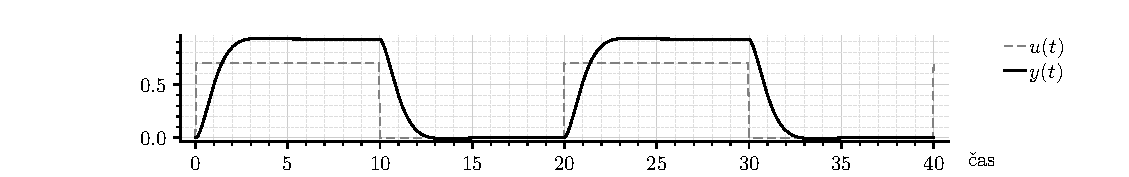
\includegraphics{figsc_ar06_MRC_lenRS_1.pdf}
	}

	\caption{Priebeh výstupnej veličiny systému \eqref{plantModelNominal} pre isté skokové priebehy vstupnej veličiny. Naozaj len mimochodom: čas je reálne v sekundách, a jednotky zobrazených veličín sú volty (via meracia karta).}
	\label{figsc_ar06_MRC_lenRS_1}

\end{figure}



Simulované priebehy vznikli s využitím nasledujúceho kódu (Python) - viď výpis kódu~\ref{vypk01}:


{\catcode`\-=12
\lstinputlisting[language=Python,
                 caption={Súbor \lstinline{ar06_prMRC_lenRS.py}},
                 label={vypk01},
				 consecutivenumbers=false,
				 linerange=c01-c01,
                 ]{../../PY/ar06_prMRC_lenRS.py}
}







% \subsubsection{Bod druhý}
\paragraph{Bod druhý}

{\color{gray}

Pre nominálnu prenosovú funkciu sústavy určte polynómy $Z_p$, $R_p$ a~zosilnenie $k_p$ pričom
\begin{equation*}
       \frac{y(s)}{u(s)} = k_p \frac{Z_p(s)}{R_p(s)}
\end{equation*}
kde $Z_p(s)$ je monický  polynóm stupňa $m$, $R_p(s)$ je monický polynóm stupňa $n$ a~$k_p$ je tzv. \emph{vysokofrekvenčné zosilnenie sústavy}. \emph{Relatívny stupeň} sústavy je $n^* = n - m$.

}

\smallskip



\begin{subequations}
    \begin{align}
        Z_p(s) &= s + 21,3809 \\
        R_p(s) &= s^2 + 2,7423 s + 2,6916 \\
        k_p &= 0,1664
    \end{align}
\end{subequations}

$Z_p(s)$ je monický polynóm, pretože pri najvyššej mocnine „premennej“ (operátor $s$) je koeficient~$1$. Rovnako polynóm $R_p(s)$ je monický. Relatívny stupeň prenosovej funkcie je $n^* = 2 - 1 = 1$








% \subsubsection{Bod tretí}
\paragraph{Bod tretí}

\smallskip

{\color{gray}

Zistite, či polynóm $Z_p(s)$ je Hurwitzov.

}

\smallskip


\noindent
Je. Hurwitzov polynóm totiž znamená, že „polynóm je stabilný“, a tým sa myslí, že korene polynómu sú v ľavej polrovine komplexnej roviny. Koreň polynómu $Z_p(s) = s + 21,3809$ je $s = -21,3809$ čo je na reálnej osi v záporných číslach, a teda v ľavej polrovine komplexnej roviny.






















% \subsubsection{Úloha druhá, poznámka k $n^*_m$}
\subsubsection{Úloha druhá}


\smallskip

{\color{gray}

Vyriešte MRC problém pre nominálnu prenosovú funkciu sústavy, uvažujte referenčný model daný prenosovou funkciou v~tvare
\begin{equation*}
    W_m(s) = \frac{s + 3}{ s^2 + 3.5 s + 3}
\end{equation*}
Referenčný model je daný prenosovou funkciou v~tvare
\begin{equation*}
    \frac{y_m(s)}{r(s)} = W_m(s) = k_m \frac{Z_m(s)}{R_m(s)}
\end{equation*}
kde $k_m$ je vysokofrekvenčné zosilnenie referenčného modelu, $Z_m(s)$ monický Hurwitzov polynóm stupňa $m_m$, $R_m(s)$ monický Hurwitzov polynóm stupňa $n_m$, pričom relatívny stupeň $n^*_m = n_m - m_m = n^*$.

Riešením MRC problému je taký zákon riadenia $u$, ktorý zabezpečí, že výstup sústavy $y$~sleduje výstup referenčného modelu $y_m$ pri danom referenčnom signály (vstupe referenčného modelu) $r$. Všeobecný tvar zákona riadenia, ktorý rieši MRC problém je
\begin{equation*}
    u = {\Theta_1^\star}^\naT \frac{\alpha(s)}{\Lambda(s)} u + {\Theta_2^\star}^\naT \frac{\alpha(s)}{\Lambda(s)} y + \Theta_3^\star y + \Theta_4^\star r
\end{equation*}
kde $\alpha(s)$ je vektor obsahujúci mocniny $s$, $\alpha(s) = \begin{bmatrix} s^{n-2}, \ldots,s, 1 \end{bmatrix}^\naT$ ak $n\geq 2$, inak $\alpha(s) = 0$. Vektory $\Theta_1^\star \in \mathbb{R}^{n-1}$, $\Theta_2^\star \in \mathbb{R}^{n-1}$ a skaláry $\Theta_3^\star \in \mathbb{R}^1$, $\Theta_4^\star \in \mathbb{R}^1$ sú konštantné parametre zákona riadenia, ktorých hodnoty hľadáme.  $\Lambda(s)$ je ľubovolný monický Hurwitzov polynóm stupňa $n-1$ obsahujúci $Z_m(s)$ ako faktor
\begin{equation*}
    \Lambda(s) = \Lambda_0(s) Z_m(s)
\end{equation*}
a teda aj $\Lambda_0(s)$ je ľubovolný monický Hurwitzov polynóm zodpovedajúceho stupňa.

}

\smallskip



Všimnime si, že dosť podstatnou vlastnosťou referenčného modelu je, že má rovnaký relatívny stupeň ako riadený systém, teda $n^*_m = n_m - m_m = n^*$. Referenčný model  nemusí mať rovnaký rád ako riadený systém. Musí však mať rovnaký relatívny stupeň. Plynie to z požiadaviek (predpokladov) pri riešení MRC problému (úlohy riadenia s referenčným modelom) vo všeobecnosti.





% \subsubsection{Bod prvý}
\paragraph{Bod prvý}

\smallskip

{\color{gray}

Na základe všeobecného tvaru zákona riadenia \eqref{C_generalControlLaw} určte zákon riadenia pre uvažovaný konkrétny prípad.

}

\smallskip


\noindent
$\alpha(s)$ je vektor, ktorého dĺžka závisí od rádu riadeného systému (zjavne má dĺžku $n-1$). V tomto prípade $n = 2$, čo spĺňa $n\geq 2$. Preto $\alpha(s) = \begin{bmatrix} s^{2-2} \end{bmatrix}^\naT = \begin{bmatrix} s^{0} \end{bmatrix}^\naT = \begin{bmatrix} 1 \end{bmatrix}^\naT = 1$. A~teda $\alpha(s)$ bude v tomto prípade jednoducho číslo $1$. Je to známa vec, nie je to parametrom zákona riadenia.

Vektory $\Theta_1^\star \in \mathbb{R}^{n-1}$, $\Theta_2^\star \in \mathbb{R}^{n-1}$ budú mať v tomto prípade tiež len jeden prvok (sú dĺžky $n-1$) a teda len rovno píšme čísla $\Theta_1^\star$ a $\Theta_2^\star$. K tomu $\Theta_3^\star$, $\Theta_4^\star$ sú vždy len skaláre. V tomto prípade sú tieto štyri čísla parametrami zákona riadenia. Tieto parametre sú predmetom výpočtu/hľadania, ak chceme použiť tento konkrétny zákon riadenia.

Polynóm $\Lambda(s)$ nie je „neznámou“. Nie je to parameter zákona riadenia v tom pravom zmysle. Je ľubovoľný ak sú dodržané uvedené podmienky/predpoklady. Pri jeho voľbe je užitočné uvažovať o tom, že tento polynóm možno interpretovať vzhľadom na \emph{pozorovateľ stavu} a jeho dynamické vlastnosti. Súvislosť pozorovateľa stavu s tu používaným zákonom riadenia bola uvedená v učebnom texte. Akokoľvek, ak $\Lambda(s)$ spĺňa dané podmienky je to ok. V tomto prípade (vlastne nie je veľa ľubovôle):
\begin{equation}
    \Lambda(s) = Z_m(s) = s + \lambda
\end{equation}
kde $\lambda = 3$, pretože $Z_m(s) = s + 3$.

Práve sme určili zákon riadenia pre uvažovaný konkrétny prípad:

\begin{equation}
	u(s) = \Theta_1^\star \frac{1}{(s + \lambda)} u(s) + \Theta_2^\star \frac{1}{(s + \lambda)} y(s) + \Theta_3^\star y(s) + \Theta_4^\star r(s)
\end{equation}








\paragraph{Bod druhý}
% \subsubsection{Bod druhý}
\label{vypocetidealparam}



\smallskip

{\color{gray}

Vypočítajte parametre $\Theta_1^\star$, $\Theta_2^\star$, $\Theta_3^\star$, $\Theta_4^\star$.

}

\smallskip

\noindent
Pre prehľadnosť označme
\begin{equation}
	\frac{y(s)}{u(s)} = k_p \frac{s + b_0}{ s^2 + a_1 s + a_0}
\end{equation}
a
\begin{equation} \label{genaralFormOfWm}
	W_m(s) = k_m \frac{s + b_{0m}}{ s^2 + a_{1m} s + a_{0m}}
\end{equation}

Potom je možné ukázať (a v učebnom texte je to ukázané), že uzavretý regulačný obvod sa bude zhodovať s referenčným modelom ak bude platiť:
\begin{subequations}
\begin{align}
	\begin{bmatrix}
		-1 & 0 & -k_p \\
		-a_1 & -k_p & -(k_p b_{0m} + k_p b_0) \\
		-a_0 & -k_p b_0 & -k_p b_0 b_{0m}
	\end{bmatrix}
	\begin{bmatrix}
    	  \Theta_1^\star \\
		  \Theta_2^\star \\
		  \Theta_3^\star
 	\end{bmatrix}
	&=
	\begin{bmatrix}
    	a_{1m} + b_0 - b_{0m} - a_1 \\
    	a_{0m} + b_0 a_{1m} - a_1 b_{0m} - a_0 \\
    	b_0 a_{0m} - a_0 b_{0m}
  	\end{bmatrix} \\
	\Theta_4^\star &= \frac{k_m}{k_p}
\end{align}
\end{subequations}

\noindent
Vypočítajme:
{\catcode`\-=12
\lstinputlisting[language=Python,
                 caption={Súbor \lstinline{ar06_prMRC_idealTh.py}},
                 label={vypk02},
				 consecutivenumbers=false,
				 linerange=c01-c01,
                 ]{../../PY/ar06_prMRC_idealTh.py}
}

\noindent
Teda:
\begin{subequations}
\begin{align}
	\begin{bmatrix}
    	  \Theta_1^\star \\
		  \Theta_2^\star \\
		  \Theta_3^\star
 	\end{bmatrix}
	&=
	\begin{bmatrix}
    	-18,3809 \\
    	11,8071 \\
    	-4,5535
  	\end{bmatrix} \\
	\Theta_4^\star &= 6,0096
\end{align}
\end{subequations}










\paragraph{Bod tretí}

% \subsubsection{Bod tretí}
\label{cast1bodtreti}

\smallskip

{\color{gray}

Zostavte simulačnú schému uzavretého regulačného obvodu a overte vypočítané parametre zákona riadenia.

}

\smallskip

\noindent
Ako realizovať numerickú simuláciu riadeného systému sme (všelijako) ukázali v~predchádzajúcom. Riadený systém je daný ako prenosová funkcia. Tú je možné previesť na opis systému v stavovom priestore a potom je možné použiť ODE solver (tak ako bolo ukázané).









\paragraph{O prevode prenosovej funkcie na opis v stavovom priestore}

Mimochodom, prevod z prenosovej funkcie na stavový opis nie je jednoznačný. Záleží na voľbe stavových veličín (stavového priestoru). Tu si dovolíme uviesť voľbu stavových veličín tak, že výsledkom je opis systému v tzv. normálnej forme riaditeľnosti.


Prenosovú funkciu riadeného systému, ktorou sa tu zaoberáme, je možné, vo všeobecnosti, napísať v tvare
\begin{align} \label{tfVseob01}
	\frac{y(s)}{u(s)} = \frac{b_1 s + b_0}{ s^2 + a_1 s + a_0}
\end{align}
pričom tu „nesedí“ označovanie a $b_0$ nie je to isté $b_0$ ako pred tým. Tu nám ide o tvar vo všeobecnosti, a ten ostal zachovaný\ldots (snáď je to pre čitateľa dostatočne jasné)

Otázka je ako túto prenosovú funkciu previesť na opis v stavovom priestore - ako zvoliť stavové veličiny. Pre prípad, keď je v čitateli len konštanta (systém nemá nuly), je voľba stavových veličín značne intuitívna. Preto napíšme prenosovú funkciu \eqref{tfVseob01} ako dve prenosové funkcie v sérii nasledovne
\begin{align}
	\frac{z(s)}{u(s)} &= \frac{1}{ s^2 + a_1 s + a_0} \label{tfVseob02a} \\
    \frac{y(s)}{z(s)} &= b_1 s + b_0 \label{tfVseob02b}
\end{align}
kde sme zaviedli pomocnú veličinu $z$.

Prvú prenosovú funkciu $\eqref{tfVseob02a}$ možno prepísať na diferenciálnu rovnicu druhého rádu v tvare
\begin{align} \label{origdifeqnz}
	\ddot z(t) + a_1 \dot z(t) + a_0 z(t) = u(t)
\end{align}
Túto je možné previesť na sústavu diferenciálnych rovníc prvého rádu - voľbou stavových veličín. Napríklad nech
\begin{align}
	x_1(t) = z(t)
\end{align}
kde $x_1(t)$ je prvá stavová veličina. Potom platí
\begin{align}
	\dot x_1(t) = \dot z(t)
\end{align}
Druhú stavovú veličinu zvoľme
\begin{align}
	x_2(t) = \dot z(t)
\end{align}
a teda
\begin{align} \label{zardrufdifr}
	\dot x_2(t) = \ddot z(t)
\end{align}
V tomto bode môžeme ľahko písať
\begin{align}
	\dot x_1(t) &= x_2(t)
\end{align}
To je prvá diferenciálna rovnica! Obsahuje len novo zavedené stavové veličiny ($x_1(t)$ a~$x_2(t)$). Druhá diferenciálna rovnica je vlastne \eqref{zardrufdifr}. Avšak, vieme signál $\ddot z(t)$ vyjadriť len pomocou novo zavedených stavových veličín? Vieme. Z \eqref{origdifeqnz} je zrejmé, že
\begin{align}
	\ddot z(t) = - a_1 \dot z(t) - a_0 z(t) + u(t) = - a_1 x_2(t) - a_0 x_1(t) + u(t)
\end{align}
takže \eqref{zardrufdifr} je
\begin{align}
	\dot x_2(t) =  - a_1 x_2(t) - a_0 x_1(t) + u(t)
\end{align}
a to je druhá diferenciálna rovnica\ldots

Obe rovnice spolu:
\begin{align}
    \dot x_1(t) &= x_2(t) \\
	\dot x_2(t) &=  - a_1 x_2(t) - a_0 x_1(t) + u(t)
\end{align}
A v maticovom zápise:
\begin{align}
	\begin{bmatrix}
    	  \dot x_1(t) \\
		  \dot x_2(t)
 	\end{bmatrix}
	&=
	\begin{bmatrix}
    	0 & 1 \\
    	- a_0 & - a_1
  	\end{bmatrix}
    \begin{bmatrix}
    	  x_1(t) \\
		  x_2(t)
 	\end{bmatrix}
    +
    \begin{bmatrix}
    	  0 \\
		  1
 	\end{bmatrix}
    u(t)
\end{align}



Vráťme sa k prenosovej funkcii \eqref{tfVseob02b}. Túto možno napísať ako diferenciálnu rovnicu v tvare
\begin{align} \label{difrov2}
    y(t) = b_1 \dot z(t) + b_0 z(t)
\end{align}
Avšak, my sme už urobili voľbu takú, že $\dot z(t) = x_2(t)$ a $z(t)= x_1(t)$. Takže diferenciálnu rovnicu \eqref{difrov2} môžme písať ako
\begin{align}
    y(t) = b_1 x_2(t) + b_0 x_1(t)
\end{align}
alebo v maticovom tvare
\begin{align}
	y(t)
	&=
	\begin{bmatrix}
    	b_0 & b_1 \\
  	\end{bmatrix}
    \begin{bmatrix}
    	  x_1(t) \\
		  x_2(t)
 	\end{bmatrix}
\end{align}

Celý systém s novo zavedenými stavovými veličinami teda je v tvare
\begin{align}
	\begin{bmatrix}
    	  \dot x_1(t) \\
		  \dot x_2(t)
 	\end{bmatrix}
	&=
	\begin{bmatrix}
    	0 & 1 \\
    	- a_0 & - a_1
  	\end{bmatrix}
    \begin{bmatrix}
    	  x_1(t) \\
		  x_2(t)
 	\end{bmatrix}
    +
    \begin{bmatrix}
    	  0 \\
		  1
 	\end{bmatrix}
    u(t)
    \\
    y(t)
    &=
    \begin{bmatrix}
        b_0 & b_1 \\
    \end{bmatrix}
    \begin{bmatrix}
          x_1(t) \\
          x_2(t)
    \end{bmatrix}
\end{align}
a ak označíme stavový vektor ako $x(t) = \begin{bmatrix} x_1(t) & x_2(t) \end{bmatrix}^\naT$, potom je systém v známom tvare
\begin{subequations} \label{susDifRovnicPreODE}
    \begin{align}
    	\dot x(t) &= A x(t) + b u(t) \\
        y(t) &= c^\naT x(t)
    \end{align}
\end{subequations}
kde matica $A$ a vektory $b$ a $c$ sú zrejmé\ldots

Sústava diferenciálnych rovníc \eqref{susDifRovnicPreODE} je vo vhodnom tvare pre potreby ODE solvera. V skripte (vo výpise kódu \ref{vypk01}) je takáto sústava realizovaná (podľa požiadaviek ODE solvera) funkciou \lstinline|fcn_LTIS()| uvedenej na riadku~\ref{fcn_LTIS}.






\paragraph{O referenčnom modeli}

Prenosová funkcia referenčného modelu je v tvare \eqref{genaralFormOfWm}. Ako túto prenosovú funkciu previesť do tvaru sústavy diferenciálnych rovníc by malo byť zrejmé z predchádzajúceho textu.

Vzhľadom na princíp fungovania tu zostavovanej simulačnej schémy (funkcia \lstinline|fcn_simSch1| vo výpise kódu~\ref{vypk01}, riadok~\ref{fcn_simSch1}), je možné realizovať numerickú simuláciu aj jednoduchšie ako to typicky predpokladá ODE solver. Pomocou jednoduchej sumácie.

Potrebujeme poznať „prírastok k stavovému vektoru“ v každej iterácii (\lstinline|for| cyklu). Tento „prírastok“ je daný veľkosťou zmeny stavového vektora (v čase) a dĺžkou času, počas ktorého táto zmena platí.

Poznáme veľkosť zmeny stavového vektora? Áno, doslova: $\dot x(t) = A x(t) + b u(t)$. V prípade referenčného modelu by sme však označili jednotlivé prvky špecifickejšie, teda $\dot x_m(t) = A_m x_m(t) + b_m r(t)$ (vstupom RM je samozrejme $r(t)$). Toto môžeme dokonca implementovať s pomocou už existujúcej funkcie \lstinline|fcn_LTIS()|:
\begin{lstlisting}[language=Python,
                    numbers=none,
                    caption={},
                    label={vypk_sht01},
                    ]
dotx_m = fcn_LTIS(x_m_log[idx-1,:], 0, A_m, b_m, ref_sig)
\end{lstlisting}



Ako dlho bude „trvať“ táto zmena? V simulačnej schéme \lstinline|fcn_simSch1| to určuje parameter (argument) \lstinline|T_s|.

„Prírastok k stavovému vektoru“ potom je \lstinline|dotx_m * T_s|. A tento prírastok je potrebné pripočítať k predchádzajúcej („starej“) hodnote stavového vektora, teda obyčajná sumácia („numerický integrál“):
\begin{lstlisting}[language=Python,
                    numbers=none,
                    caption={},
                    label={vypk_sht02},
                    ]
x_m_log[idx,:] = x_m_log[idx-1,:] + dotx_m * T_s
\end{lstlisting}
Tým sme získali hodnotu stavového vektora v aktuálnom kroku („novú“ hodnotu). My však v tomto prípade potrebujeme výstupnú veličinu (nie stavový vektor), teda
\begin{lstlisting}[language=Python,
                    numbers=none,
                    caption={},
                    label={vypk_sht03},
                    ]
y_m_log[idx,:] = np.dot(c_m.T, x_m_log[idx,:].reshape(-1,1))
\end{lstlisting}
kde by mali byť jednotlivé premenné (a funkcie) viac-menej už čitateľovi jasné\ldots\  Snáď len toľko, že \lstinline|c_m.T| je transponované pole \lstinline|c_m| a že \lstinline|reshape(-1,1)| je metóda, ktorá zmení tvar poľa na toľko riadkov koľko treba (prvý argument \lstinline|-1|) a práve jeden stĺpec (druhý argument \lstinline|1|).







\paragraph{O zákone riadenia}

Zákon riadenia má v tomto prípade tvar - viď \eqref{controlLaw}. To je však zápis vo frekvenčnej oblasti s operátorom $s$.

Tu však potrebujeme zákon riadenia v časovej oblasti. Dovolíme si preto písať
\begin{equation} \label{controlLawTimeDomain}
	u(t) = \Theta_1^\star  \left[ \frac{1}{(s + \lambda)} \right] u(t)
    + \Theta_2^\star \left[ \frac{1}{(s + \lambda)} \right] y(t)
    + \Theta_3^\star y(t) + \Theta_4^\star r(t)
\end{equation}
kde sme zmiešali písanie operátora $s$ a času $t$.

Autor pozná takýto (alebo podobný) spôsob zápisu práve z literatúry o klasickom adaptívnom riadení\footnote{viď napr. knihu G. Tao., Adaptive control design and analysis. \cite{Tao03}}. Tu nie je cieľom porušovať matematické vzťahy a podobne. Tu je cieľom zjednodušene vyjadriť praktický zápis, akým je \eqref{controlLawTimeDomain}, vo vzťahu k pôvodnej teórii daného zákona riadenia (kde mimochodom je takýto zápis veľmi užitočný)

Autor sa však mnoho krát stretáva s nevôľou čitateľov/poslucháčov prijať uvedený spôsob zápisu, prípadne si to vyžaduje dodatočné vysvetľovanie.





Akokoľvek, čo vlastne predstavuje napríklad prvý člen na pravej strane rovnice \eqref{controlLawTimeDomain}? Ešte lepšie, prvý člen na pravej strane rovnice \eqref{controlLaw}? Označme prvý člen na pravej strane rovnice \eqref{controlLaw} takto:
\begin{align}
	y_{\nu_1}(s) = \Theta_1^\star \frac{1}{(s + \lambda)} u(s)
\end{align}
Je to teda samostatný dynamický systém daný prenosovou funkciou. Vstupom je v~tomto prípade signál $u(s)$. Tento signál je „filtrovaný“ vždy známym filtrom, ktorého vlastnosti sú dané polynómom $\Lambda(s)$. Vznikne „nový signál“ (prefiltrované $u$) a tento je potom vynásobený parametrom zákona riadenia, v tomto prípade $\Theta_1^\star$. Uvedený samostatný dynamický systém je možné vyjadriť aj opisom v stavovom priestore. Pre tento konkrétny príklad
\begin{subequations}
    \begin{align}
         \dot \nu_1(t) &= -\lambda \nu_1(t) + u(t) \\
         y_{\nu_1}(t) &= \Theta_1^\star \nu_1(t)
    \end{align}
\end{subequations}
kde sme zaviedli pomocnú stavovú veličinu $\nu_1(t)$. Vieme aj reálne generovať (vyrobiť) tento pomocný signál $\nu_1(t)$? Je to jednoducho stavová veličina lineárneho dynamického systému, v princípe rovnakého ako je referenčný model, alebo model riadeného systému. Takže vieme reálne generovať pomocný signál $\nu_1(t)$. Prvý člen zákona riadenia \eqref{controlLawTimeDomain} teda nahrádza výraz
\begin{align}
     \Theta_1^\star \nu_1(t)
\end{align}
pričom $\nu_1(t)$ je signál, ktorý vieme vyrobiť\ldots

Druhý člen zákona riadenia \eqref{controlLawTimeDomain}, analogicky, nahrádza výraz
\begin{align}
     \Theta_2^\star \nu_2(t)
\end{align}
kde $\nu_2(t)$ je daný diferenciálnou rovnicou
\begin{align}
     \dot \nu_2(t) &= -\lambda \nu_2(t) + y(t)
\end{align}

Zákon riadenia \eqref{controlLawTimeDomain} je teda možné zapísať v tvare
\begin{equation} \label{controlLawTimeDomain2}
	u(t) = \Theta_1^\star \nu_1(t)
    + \Theta_2^\star \nu_2(t)
    + \Theta_3^\star y(t) + \Theta_4^\star r(t)
\end{equation}
Čo sú parametre a čo sú signály v tomto zákone riadenia? Rozdeľme ich do vektorov. Vektora parametrov a vektora signálov
\begin{align}
    u(t) =
    \begin{bmatrix}
          \Theta_1^\star & \Theta_2^\star & \Theta_3^\star & \Theta_4^\star
    \end{bmatrix}
    \begin{bmatrix}
          \nu_1(t) \\ \nu_2(t) \\ y(t) \\ r(t)
    \end{bmatrix}
\end{align}
a označme
\begin{align}
    u(t) = {\Theta^\star}^\naT \omega
\end{align}
Vieme vyrobiť všetky signály v signálnom vektore $\omega$? Vieme. Poznáme parametre vo vektore $\Theta^\star$? Poznáme.

V tejto chvíli nič nebráni zostaveniu simulačnej schémy uzavretého regulačného obvodu.













\paragraph{O formálnej súvislosti s MRAC stavovým}

Pre lepšiu konzistenciu uvedeného s učebným textom je vhodné zmeniť poradie prvkov v signálnom vektore $\omega$. Učebný text totiž pracuje s myšlienkou čo najviac pripodobniť odvodenie „MRAC vstupno-výstupného“ k odvodeniu, ktoré definuje „MRAC stavový“. Dôvodom je, že ak máme k dispozícii stavový opis systému práve v normálnej forme riaditeľnosti, potom odvodenie (viac-menej akéhokoľvek) zákona riadenia je najjednoduchšie možné po formálnej stránke. Najpriamočiarejšie. Bez nutnosti formulácie predpokladov navyše, formálnych konštrukcií a podobne.

Inými slovami, ak máme dostupný postup návrhu (odvodenie) nejakého riadiaceho systému, v tomto prípade Adaptívneho riadenia s referenčným modelom s využitím Lyapunovovej teórie stability, potom je veľmi výhodné snažiť sa tento postup uplatniť vo všeobecnosti.

Ak tento postup máme pri predpoklade, že sú dostupné práve tie stavové veličiny, ktoré vedú na opis riadeného systému práve v normálnej forme riaditeľnosti, potom by bolo výhodné aby sme „novú úlohu“ formálne previedli do tvaru, ktorý zodpovedá známemu postupu.

To sa deje pri odvodení „MRAC vstupno-výstupného“ práve vtedy, keď sa zavedie pojem \emph{doplnená sústava}, alebo \emph{doplnený riadený systém}. To má čitateľ možnosť vidieť v učebnom texte. „Doplnkom“ sú práve signály, ktoré sme tu označili ako $\nu_1(t)$ a $\nu_2(t)$.

Výsledkom je, že zákon riadenia sa uvažuje v tvare
\begin{equation} \label{vsZakonRiadeniaMaticMRCp2}
	u(t) = {\Theta_c^\star}^\naT D X(t) + \Theta_4^\star r(t)
\end{equation}
kde $ \Theta_c^\star = \begin{bmatrix} \Theta_3^\star & {\Theta_1^\star}^\naT & {\Theta_2^\star}^\naT \end{bmatrix}^\naT; \; \Theta_4^\star $ sú parametre zákona riadenia a maticu
\begin{align*}
	D = \begin{bmatrix} c^\naT & 0 & 0 \\ 0 & I & 0 \\ 0 & 0 & I \end{bmatrix}
\end{align*}
sme zaviedli práve preto aby sme v zákone riadenia \eqref{vsZakonRiadeniaMaticMRCp2} mohli priamo písať doplnený stavový vektor $X(t)$, teda
\begin{align}
    X(t) = \begin{bmatrix} x(t) \\ \nu_1(t) \\ \nu_2(t) \end{bmatrix}
\end{align}
Všimnime si ale, že
\begin{align}
    DX(t) = \begin{bmatrix} y(t) \\ \nu_1(t) \\ \nu_2(t) \end{bmatrix}
\end{align}
čo je veľmi dôležité, pretože signál $y(t)$ máme, ale signál $x(t)$ (pochopiteľne) nemáme.

Pre prípad \eqref{vsZakonRiadeniaMaticMRCp2} teda môžeme zaviesť signálny vektor $\omega$ v poradí:
\begin{align}
    \omega =
    \begin{bmatrix}
          DX(t) \\  r(t)
    \end{bmatrix}
    =
    \begin{bmatrix}
          y(t) \\ \nu_1(t) \\ \nu_2(t) \\  r(t)
    \end{bmatrix}
\end{align}
Ak raz zvolíme poradie signálov vo vektore $\omega$, potom je tým jednoznačne určené aj poradie signálov vo vektore parametrov, v tomto prípade
\begin{align}
    \Theta =
    \begin{bmatrix}
          \Theta_3^\star \\ \Theta_1^\star \\ \Theta_2^\star \\ \Theta_4^\star
    \end{bmatrix}
\end{align}









\paragraph{O simulačnej „schéme“ (skôr o „simulačnom skripte“)}

Nasledujúci výpis kódu~\ref{vypk06} obsahuje funkciu \lstinline|fcn_simSch2|. Je postavená na rovnakých princípoch ako sme videli v kóde~\ref{vypk01}. Navyše však obsahuje aj realizáciu neadaptívnej verzie riadiaceho systému, ktorý používa tu diskutovaný zákon riadenia.

Overenie správnosti vypočítaných parametrov zákona riadenia je realizované grafickým porovnaním priebehu výstupu referenčného modelu a výstupnej veličiny riadeného systému - viď obr.~\ref{figsc_ar06_MRC_1}.




\begin{figure}[!t]
    \centering

    \makebox[\textwidth][c]{%
    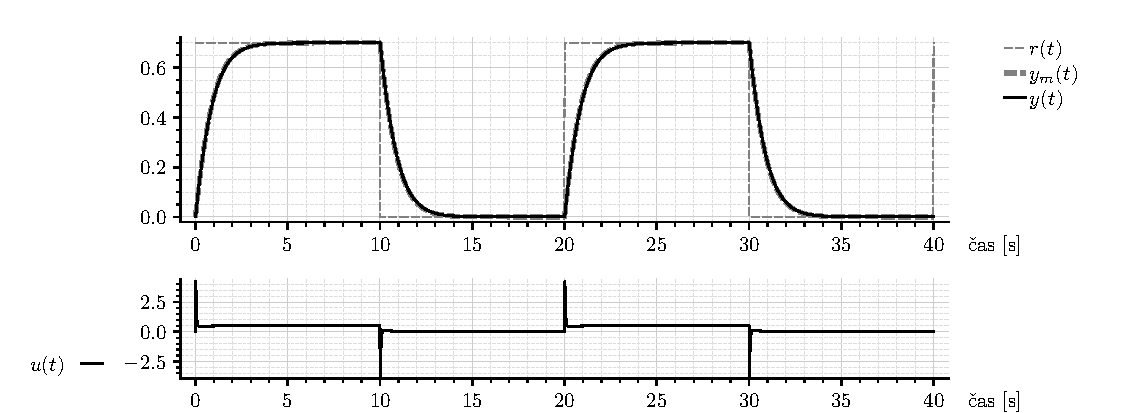
\includegraphics{figsc_ar06_MRC_1.pdf}
    }

    \caption{Porovnanie priebehu výstupu referenčného modelu a výstupnej veličiny riadeného systému}
    \label{figsc_ar06_MRC_1}

\end{figure}







{\catcode`\-=12
\lstinputlisting[language=Python,
                 caption={Súbor \lstinline{ar06_prMRC.py}, simulačná schéma uzavretého regulačného obvodu},
                 label={vypk06},
				 consecutivenumbers=false,
				 linerange=c01-c01,
                 ]{../../PY/ar06_prMRC.py}
}









































\section{SPR prenosové funkcie, MKY lemma}



\subsection{Striktne pozitívne reálne prenosové funkcie}


Pojem \emph{Pozitívne reálna} (PR) a \emph{Striktne pozitívne reálna} (SPR) prenosová funkcia zohráva dôležitú úlohu v analýze stability nie len adaptívnych systémov \cite{IF06}. Je preto dôležité disponovať kritériom, ktoré umožní zistiť, či príslušná prenosová funkcia je SPR (\cite{MH93} str. 164).

Podľa definície 3.5.1 a 3.5.2 v \cite{IF06}, str. 127, prenosová fukcia $G(s)$ komplexnej premennej $s$ sa nazýva pozitívne reálna (PR) ak
\begin{enumerate}
	\item $G(s)$ je reálna pre reálne $s$.
	\item $\Re \left\{ G(s) \right\} \geq 0$ pre všetky $\Re \left\{ s \right\} > 0$.
\end{enumerate}
Prenosová funkcia $G(s)$ je striktne pozitívne reálna (SPR) ak existuje reálne kladné číslo $\varepsilon$ také, že $G(s - \varepsilon)$ je PR.

Prakticky nie je jednoduché zistiť, či uvedené podmienky sú splnené. V~nasledujúcom uvedieme ekvivalentné nutné a~postačujúce podmienky pozitívnej reálnosti. Platnosť týchto podmienok sa dá ľahko overiť.
Prenosová funkcia $G(s)$ je PR keď vyhovuje všetkým nasledujúcim podmienkam
\begin{enumerate}
	\item $G(s)$ je reálna pre všetky reálne~$s$.
	\item Menovateľ $G(s)$ má korene  v~ľavej polrovine komplexnej roviny alebo má reálne korene na imaginárnej osi.
	\item $\Re \left\{ G(j\omega) \right\} \geq 0$ pre všetky reálne $\omega$.
\end{enumerate}

\noindent
Pre vyjadrenie reálnej časti funkcie $G(j\omega)$ je výhodné využiť, že platí:
\begin{equation*}
	\frac{a + jb}{c + jd} = \frac{(a + jb) (c - jd)}{(c + jd) (c - jd)} = \frac{(a + jb) (c - jd)}{c^2 + d^2}
\end{equation*}








\subsection{Meyerova-Kalmanova-Yakubovichova Lemma}
\label{Meyer-Kalman-Yakubovichova Lemma}


Pre danú stabilnú maticu $A$, vektory $b$, $c$ a skalár $d \geq 0$, platí nasledujúce: Ak
\begin{equation*}
	G(s) = d + c^\naT \left( s I - A \right)^{-1} b
\end{equation*}
je SPR, potom pre danú maticu $L = L^\naT > 0$ existujú skalár $v > 0$, vektor $q$ a matica $P =P^\naT > 0$ také, že
\begin{align*}
	A^\naT P + P A &= - q q^\naT - v L \\
	P b	- c	&= \pm q \sqrt{2d}
\end{align*}
Tak znie veta, ktorá, ako sa ukáže, je veľmi užitočná pri návrhu MRAC využívajúceho len vstupno-výstupné informácie.

V tomto kurze ju využijeme v menej všeobecnom tvare: Nech je systém daný trojicou $A_c$, $\overline{B}_c$, $C_c$ a $A_c$ nech je stabilná matica. Ak $ W_m(s) = C_c^\naT \left(  s I - A_c \right)^{-1} \overline{B}_c $ je SPR, potom platí, že
\begin{align*}
	  A_c^\naT P + P A_c &= - Q\\
	  P \overline{B}_c &= C_c
\end{align*}
kde $Q = Q^\naT > 0$. A je to práve fakt, že ak je $W_m(s)$ SPR tak platí $P \overline{B}_c = C_c$, ktorý umožní zredukovať zákon adaptácie tak, že v ňom vystupuje len odchýlka výstupných veličín sústavy a referenčného modelu \cite{Mon74}.













\section{Adaptačná odchýlka}



\subsection{Model sústavy a referenčný model}

Uvažujme sústavu opísanú prenosovou funkciou v tvare
\begin{equation} \label{vvMRAC_PFSustavy}
	\frac{y(s)}{u(s)} = 	k_p 	\frac{Z_p(s)}{R_p(s)}
\end{equation}
kde $Z_p(s)$ je monický Hurwitzov polynóm stupňa $m$, $R_p(s)$ je monický polynóm stupňa $n$ a $k_p$ je tzv. \emph{vysokofrekvenčné zosilnenie sústavy}. \emph{Relatívny stupeň} sústavy je $n^* = n - m$. Predpokladajme, že relatívny stupeň $n^*$ sústavy je známy. Pre zjednodušenie tiež predpokladajme, že aj stupne $n$ a $m$ polynómov sú známe, pričom vo všeobecnosti známe nemusia byť. Koeficienty polynómov $Z_p(s)$ a $R_p(s)$ (parametre sústavy) sú neznáme. Hodnota a znamienko zosilnenia $k_p$ nech je známe.

Sústava v tvare \eqref{vvMRAC_PFSustavy} môže byť reprezentovaná opisom v stavovom priestore v~tvare
\begin{subequations}  \label{vvMRACStavOpisSust}
	\begin{align}
		 \dot x  &= A x + b u \\
		 y &= c^\naT x
	\end{align}
\end{subequations}
kde $x$ je vektor stavových veličín sústavy a $A$, $b$, $c^\naT$ sú matice (vektory) zodpovedajúcich rozmerov pričom hodnoty ich prvkov sú neznáme.

Cieľom riadenia je: Nech všetky signály uzavretého regulačného obvodu sú ohraničené a výstupná veličina $y$ sústavy nech sleduje výstupnú veličinu referenčného modelu, ktorý je daný prenosovou funkciou v tvare
\begin{equation} \label{vvMRAC_PFRefModel}
	\frac{y_m(s)}{r(s)} = W_m(s) = k_m \frac{Z_m(s)}{R_m(s)}
\end{equation}
kde $k_m$ je vysokofrekvenčné zosilnenie, $Z_m(s)$ monický Hurwitzov polynóm stupňa $m_m$, $R_m(s)$ monický Hurwitzov polynóm stupňa $n_m$, pričom relatívny stupeň $n^*_m = n_m - m_m = n^*$. Všetky parametre (koeficienty polynómov a $k_m$) referenčného modelu sú známe, dané \uv{projektantom}.









\subsection{Zákon riadenia}

Ako bolo ukázané v predchádzajúcich témach predmetu, zákon riadenia v tvare
\begin{equation} \label{vvMRAC_vseobZakRiaď_i}
	u = {\Theta_1^\star}^\naT \frac{\alpha(s)}{\Lambda(s)} u + {\Theta_2^\star}^\naT \frac{\alpha(s)}{\Lambda(s)} y + \Theta_3^\star y + \Theta_4^\star r
\end{equation}
zabezpečí, že priebeh výstupnej veličiny $y$ sa zhoduje s~priebehom výstupnej veličiny referenčného modelu $y_m$~ak sú parametre zákona vypočítané z podmienok zhody
\begin{subequations}
	\begin{align} \label{vvMRAC_idealTh4}
		\Theta_4^\star &= \frac{k_m}{k_p} \\
		\Lambda &= \Lambda_0 Z_m  \label{vvMRAC_idealLambda} \\
		R_p \left( \Lambda - {\Theta_1^\star}^\naT \alpha(s) \right) -  k_p Z_p 	\left( {\Theta_2^\star}^\naT  \alpha(s) +  \Theta_3^\star\Lambda	 \right) &= Z_p \Lambda_0 R_m
	\end{align}
\end{subequations}

Pretože parametre sústavy \eqref{vvMRAC_PFSustavy} sú neznáme, zákon riadenia \eqref{vvMRAC_vseobZakRiaď_i} nemožno použiť. Použije sa zákon riadenia v tvare
\begin{equation} \label{vvMRAC_vseobZakRiad}
	u = \Theta_1^\naT \frac{\alpha(s)}{\Lambda(s)} u + \Theta_2^\naT \frac{\alpha(s)}{\Lambda(s)} y + \Theta_3 y + \Theta_4 r
\end{equation}
kde $\Theta_1$, $\Theta_2$, $\Theta_3$ a $\Theta_4$ sú odhadmi ideálnych parametrov $\Theta_1^\star$, $\Theta_2^\star$, $\Theta_3^\star$ a $\Theta_4^\star$ v každom čase $t$. Je potrebné nájsť zákon adaptácie, ktorý priebežne generuje (identifikuje) hodnoty $\Theta_1(t)$, $\Theta_2(t)$, $\Theta_3(t)$ a $\Theta_4(t)$.

Pomocné filtre vystupujúce v~zákone riadenia v~stavovom priestore sú (viď predch. článok)
\begin{subequations} \label{vvMRAC_pomFiltre}
	\begin{align}
		\dot \nu_1 &= \Lambda \nu_1 + q u \\
		\dot \nu_2 &= \Lambda \nu_2 + q c^\naT x
	\end{align}
\end{subequations}
a uvažovaný zákon riadenia je
\begin{equation}	\label{vvMRAC_uvZakRiad}
	u = \Theta_c^\naT D X + \Theta_4 r
\end{equation}
kde $ \Theta_c = \begin{bmatrix} \Theta_3^\star  & \Theta_1^\naT & \Theta_2^\naT \end{bmatrix}^\naT$, $\Theta_4$ sú parametre zákona riadenia a
\begin{align*}
	D = \begin{bmatrix} c^\naT & 0 & 0 \\ 0 & I & 0 \\ 0 & 0 & I \end{bmatrix}
\end{align*}







\subsection{Rovnica adaptačnej odchýlky}



Pridanie pomocných filtrov \eqref{vvMRAC_pomFiltre} k stavovému opisu sústavy \eqref{vvMRACStavOpisSust} vedie k \uv{doplnenej sústave} (viď predch. časti predmetu) v tvare
\begin{subequations} \label{vvMRAC_doplnSustava}
	\begin{align}
		\dot X &=  A_o  X + B_c u \\
		y &= C_c^\naT  X
	\end{align}
\end{subequations}
Parametrizácia doplnenej sústavy \eqref{vvMRAC_doplnSustava} pomocou ideálnych parametrov zákona riadenia sa dosiahne pripočítaním a odpočítaním ideálneho vstupného výrazu $B_c u^\star = B_c {\Theta_c^\star}^\naT D  X + B_c \Theta_4^\star r $
\begin{subequations} \label{vvMRAC_doplnSustava_02}
	\begin{align}
		\dot X &= A_o X + B_c u +  B_c {\Theta_c^\star}^\naT D   X  + B_c  \Theta_4^\star  r - B_c {\Theta_c^\star}^\naT D   X  -  B_c  \Theta_4^\star  r	\\
		\dot X &= \left( A_o + B_c {\Theta_c^\star}^\naT D \right)  X + B_c  \Theta_4^\star r + B_c \left( u - {\Theta_c^\star}^\naT D  X - \Theta_4^\star  r \right)	  \label{vvMRAC_paramDopnSustmedzivyp}
	\end{align}
\end{subequations}
Z predchádzajúcich častí vieme, že $ A_c = A_o + B_c {\Theta_c^\star}^\naT D $, $\overline{B}_c = B_c \Theta_4^\star$ a tiež, že neminimálnu reprezentáciu referenčného modelu \eqref{vvMRAC_PFRefModel} možno (teoreticky) zapísať v~tvare
\begin{subequations} \label{vvMRAC_NeminRefModel}
	\begin{align}
		\dot X_m &= A_c X_m + \overline{B}_c r \\
		y_m &= C_c^\naT X_m
	\end{align}
\end{subequations}
Potom parametrizovaná doplnená sústava \eqref{vvMRAC_paramDopnSustmedzivyp} je
\begin{subequations}
\label{vvMRAC_ParametrizovanaDoplnSustava}
	\begin{align}
		\dot X &= A_c X + \overline{B}_c r + \overline{B}_c \frac{1}{\Theta_4^\star} \left( u - {\Theta_c^\star}^\naT D  X - \Theta_4^\star r \right) \\
		y &= C_c^\naT  X
	\end{align}
\end{subequations}

Definujme \emph{adaptačnú odchýlku} v tvare
\begin{align}
	e &=  X -  X_m \\
	e_1 & = y - y_m
\end{align}
potom:
\begin{subequations} \label{vvMRAC_adaptOdchmedzi}
	\begin{align}
		\dot X - \dot X_m &= A_c \left( X -  X_m \right) + \overline{B}_c r - \overline{B}_c r + \overline{B}_c \frac{1}{\Theta_4^\star} \left( u - {\Theta_c^\star}^\naT D   X - \Theta_4^\star  r \right) \\
		y - y_m &= C_c^\naT \left(  X - X_m \right)
	\end{align}
\end{subequations}
a teda
\begin{subequations}
\label{vvMRAC_adaptOdchSS}
	\begin{align}
		\dot{e} &= A_c e + \overline{B}_c \frac{1}{\Theta_4^\star} \left( u - {\Theta_c^\star}^\naT D   X - \Theta_4^\star r \right) \\
		e_1  &= C_c^\naT e
	\end{align}
\end{subequations}
čo je základná rovnica opisujúca dynamiku adaptačnej odchýlky v stavovom priestore, ktorú možno vyjadriť v~tvare prenosovej funkcie uvážením, že platí
\begin{equation}
	W_m(s) = C_c^\naT \left( s I - A_c \right)^{-1} \overline{B}_c
\end{equation}
Potom \eqref{vvMRAC_adaptOdchSS} v tvare prenosovej funkcie je
\begin{equation} \label{vvMRAC_adaptOdchTF}
	e_1 = W_m(s)  \frac{1}{\Theta_4^\star} \left( u - {\Theta_c^\star}^\naT D  X - \Theta_4^\star r \right)
\end{equation}

Odhadom odchýlky $e_1$ nech je $\hat{e}_1$, ktorá je závislá od odhadov $\Theta_c(t)$, $\Theta_4(t)$.
\begin{equation} \label{vvMRAC_odhadAdaptOdch}
	\hat{e}_1 = W_m(s)  l \left( u - \Theta_c D  X - \Theta_4 r \right)
\end{equation}
kde $l$ je odhadom hodnoty $\frac{1}{\Theta_4^\star}$. Pretože uvažujeme zákon riadenia $ u = \Theta_c^\naT D X + \Theta_4 r $, tak $\hat{e}_1 = 0; \; \forall t$. To znamená, že rovnica \eqref{vvMRAC_odhadAdaptOdch} nie je potrebná pre identifikáciu neznámych parametrov $\Theta_c^\star$, $\Theta_4^\star$ a ako chybu odhadu týchto parametrov možno použiť priamo rovnicu adaptačnej odchýlky \eqref{vvMRAC_adaptOdchTF}.




















\section{Zákon adaptácie pri $n^* = 1$}


Uvažujme, že relatívny stupeň sústavy \eqref{vvMRAC_PFSustavy} je $n^* = 1$. Prenosová funkcia referenčného medelu $W_m(s)$ sa volí tak, aby jej relatívny stupeň bol zhodný s relatívnym stupňom sústavy. Relatívny stupeň referenčného modelu $n_m^* = 1$ umožňuje aby prenosová funkcia $W_m(s)$ bola navrhnutá ako striktne pozitívne reálna (SPR).

Nech $W_m(s) = C_c^\naT \left( s I - A_c \right)^{-1} \overline{B}_c$ je SPR. Potom podľa MKY lemmy v časti \ref{Meyer-Kalman-Yakubovichova Lemma} existuje taká matica $P$, pre ktorú platí
\begin{subequations} \label{vvMRAC_dosledkyMKYlemmy}
	\begin{align}
		A_c^\naT P  +  P  A_c  &=  - Q \\
		P  \overline{B}_c &=   C_c
	\end{align}
\end{subequations}
kde $Q = Q^\naT > 0$. Táto skutočnosť sa v ďalšom využije pri voľbe kandidáta na Lyapunovovu funkciu.

Dosadením \eqref{vvMRAC_uvZakRiad} za $u$ do \eqref{vvMRAC_adaptOdchTF} máme
\begin{equation} \label{vvMRAC_adaptOdchmedziDefTF}
	e_1 = W_m(s) \frac{1}{\Theta_4^\star} \left( \theta_c^\naT D X + \theta_4 r \right)
\end{equation}
kde $\theta_c = \Theta_c - \Theta_c^\star$ a $\theta_4 = \Theta_4 - \Theta_4^\star$. Zavedením vektora chyby nastavenia parametrov zákona riadenia $\theta = \begin{bmatrix}  \theta_c^\naT & \theta_4 \end{bmatrix}^\naT$ a signálneho vektora $\omega = \begin{bmatrix} (D X)^\naT & r \end{bmatrix}^\naT$ máme známy tvar adaptačnej odchýlky
\begin{equation} \label{vvMRAC_adaptOdchDefTF}
	e_1 = W_m(s)  \frac{1}{\Theta_4^\star} \left( \theta^\naT \omega \right)
\end{equation}
alebo
\begin{subequations} \label{vvMRAC_adaptOdchDefSS}
	\begin{align}
		\dot{e} &= A_c e + \overline{B}_c \frac{1}{\Theta_4^\star} \left( \theta^\naT \omega \right) \\
		e_1 &= C_c^\naT e
	\end{align}
\end{subequations}

V tomto prípade rovnica \eqref{vvMRAC_adaptOdchDefTF} alebo \eqref{vvMRAC_adaptOdchDefSS} dáva do vzťahu chybu nastavenia parametrov zákona riadenia $\Theta$ a~adaptačnú odchýlku $e_1$ cez SPR prenosovú funkciu.

Predpokladajme, že štruktúra zákona adaptácie je daná diferenciálnou rovnicou všeobecne zapísanou v~tvare
\begin{equation}
	\dot{\theta} = f(e_1, \omega)
\end{equation}
teda aby zákon adaptácie bol funkciou len výstupnej adaptačnej odchýlky $e_1$ a nie aj jej derivácií $e$, pretože tieto nie sú dostupné, nakoľko nie sú dostupné stavové veličiny sústavy.







\begin{figure}[t]
	\centering

	\makebox[\textwidth][c]{%
	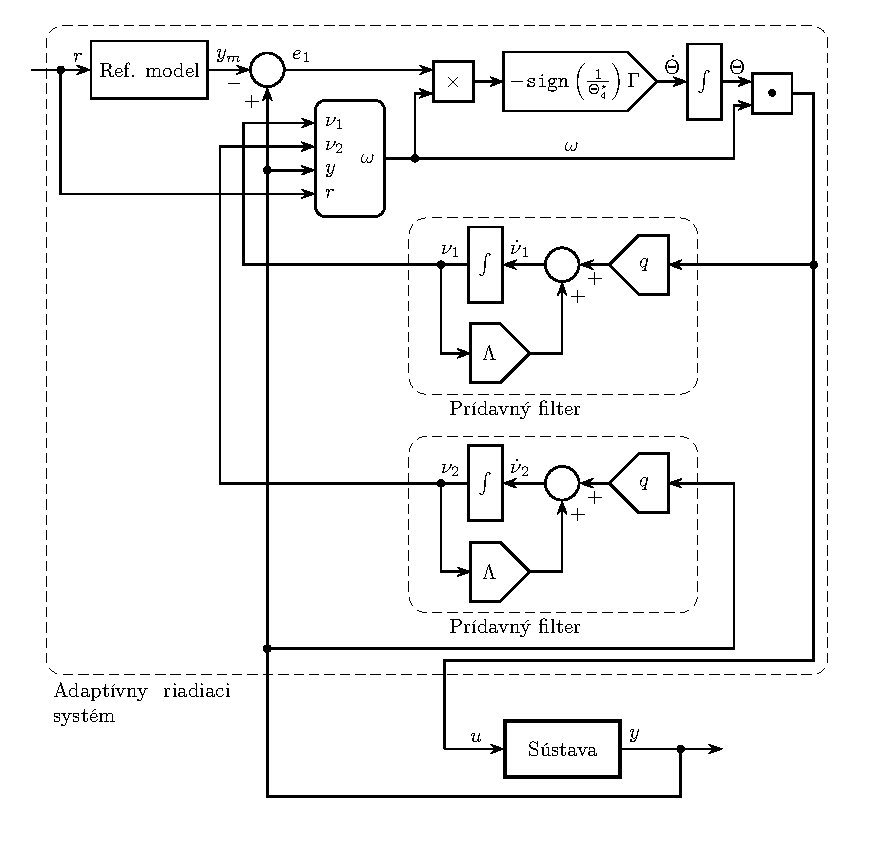
\includegraphics{Obr_vvARS_standalone.pdf}
	}

	\caption{Bloková schéma MRAC so vstupno-výstupnou štruktúrou riadenia pri $n^\star = 1$}
	\label{Bloková schéma MRAC so vstupno-výstupnou štruktúrou riadenia}
\end{figure}






Zvoľme kandidáta na Ljapunovovu funkciu v tvare
\begin{equation}
	V = e^\naT P e + \left| \frac{1}{\Theta_4^\star} \right| \theta^\naT \Gamma^{-1} \theta
\end{equation}
kde $\Gamma > 0$ je ľubovolná diagonálna matica, $\left| \frac{1}{\Theta_4^\star} \right|$ je absolútna hodnota prevrátenej hodnoty parametra $\Theta_4^\star$ a~$P = P^\naT>0$ spĺňa rovnice \eqref{vvMRAC_dosledkyMKYlemmy}, ktoré vyplývajú z~MKY lemmy.
\begin{equation}
	\dot{V} = \dot{e}^\naT P e + e^\naT P \dot{e} + \left| \frac{1}{\Theta_4^\star} \right| \left( \dot{\theta}^\naT \Gamma^{-1} \theta + \theta^\naT \Gamma^{-1} \dot{\theta} \right)
\end{equation}
Poznáme \eqref{vvMRAC_adaptOdchDefSS} odkiaľ $ \dot{e}^\naT = e^\naT A_c^\naT + \omega^\naT \theta \frac{1}{\Theta_4^\star} \overline{B}_c^\naT $, po dosadení týchto výrazov:
\begin{align}
	\dot{V} &= \left( e^\naT A_c^\naT + \omega^\naT \theta \frac{1}{\Theta_4^\star} \overline{B}_c^\naT \right) P e  + e^\naT P \left( A_c  e + \overline{B}_c \frac{1}{\Theta_4^\star} \theta^\naT \omega \right) +  2 \left| \frac{1}{\Theta_4^\star} \right| \theta^\naT \Gamma^{-1} \dot{\theta} \\
	\dot{V} &= e^\naT \left( - Q \right) e + 2 e^\naT P \overline{B}_c \frac{1}{\Theta_4^\star} \theta^\naT \omega + 2 \left| \frac{1}{\Theta_4^\star} \right| \theta^\naT \Gamma^{-1} \dot{\theta}
\end{align}
Pripomeňme, že platí $P \overline{B}_c = {C_c}$ (to vďaka tomu, že $W_m(s)$ je SPR), potom
\begin{align}
	\dot{V} &= e^\naT \left( - Q \right) e + 2 e^\naT C_c \frac{1}{\Theta_4^\star} \theta^\naT \omega + 2 \left| \frac{1}{\Theta_4^\star} \right| \theta^\naT \Gamma^{-1} \dot{\theta}
\end{align}
Všimnime si, že $e^\naT C_c = C_c^\naT e = e_1$. Práve tento moment umožní aby zákon adaptácie $\dot{\theta} = f(e_1, \omega)$ bol funkciou $e_1$ a nie $e$. Časová derivácia $\dot{V}$
\begin{align}
	\dot{V} &= e^\naT \left( - Q \right) e + 2 e_1 \frac{1}{\Theta_4^\star} \theta^\naT \omega + 2 \left| \frac{1}{\Theta_4^\star} \right| \theta^\naT \Gamma^{-1} \dot{\theta}
\end{align}
bude záporne definitná ak
\begin{subequations}
	\begin{align}
    	0 &= 2 e_1 \frac{1}{\Theta_4^\star} \theta^\naT \omega + 2 \left| \frac{1}{\Theta_4^\star} \right| \theta^\naT \Gamma^{-1} \dot{\theta} \\
    	2 \left| \frac{1}{\Theta_4^\star} \right| \theta^\naT G^{-1} \dot{\theta} &= - 2 e_1 \frac{1}{\Theta_4^\star} \Theta^\naT \omega \\
    	\left| \frac{1}{\Theta_4^\star} \right| \Gamma^{-1} \dot{\theta} &= - e_1 \, \texttt{sign}\left(\frac{1}{\Theta_4^\star}\right) \left| \frac{1}{\Theta_4^\star} \right| \omega \\
    	\Gamma^{-1} \dot{\theta} &= - \texttt{sign}\left(\frac{1}{\Theta_4^\star}\right) e_1 \omega \\
    	\dot{\theta} &= - \texttt{sign}\left(\frac{1}{\Theta_4^\star}\right) e_1 \Gamma \omega
	\end{align}
\end{subequations}
Rovnako ako sme zaviedli vektor $\Theta$, zavedieme aj vektor parametrov zákona riadenia v tvare \\ $\Theta = \begin{bmatrix} \Theta_c^\naT & \Theta_4 \end{bmatrix}^\naT = \begin{bmatrix} {\Theta}_3 & \Theta_1^\naT & \Theta_2^\naT & \Theta_4 \end{bmatrix}^\naT$ a vektor $\omega$ možno zapísať v tvare $\omega = \begin{bmatrix} y & \nu_1^\naT & \nu_2^\naT & r \end{bmatrix}^\naT$. Potom zákon adaptácie je
\begin{equation}
	\dot{\Theta} = - \texttt{sign}\left(\frac{1}{\Theta_4^\star}\right) \Gamma e_1 \omega
\end{equation}
a uvažovaný zákon riadenia možno zapísať v tvare $u = \Theta^\naT \omega$.














\section{Zákon adaptácie pri $n^* = 2$}



\subsection{Priamočiary postup}



Uvažujme relatívny stupeň sústavy \eqref{vvMRAC_PFSustavy} $n^* = 2$. Prenosová funkcia referenčného medelu $W_m(s)$ sa volí tak, aby jej relatívny stupeň bol zhodný s relatívnym stupňom sústavy, teda $n_m^* = 2$. To ale znamená (bez dôkazu), že prenosová funkcia $W_m(s)$ nie je SPR. Preto nie je možné použiť predchádzajúci postup a je ho potrebné modifikovať.

Rovnica pre adaptačnú odchýlku \eqref{vvMRAC_adaptOdchTF}
\begin{equation} \label{vvMRAC_adaptOdchTFn2}
	e_1 = W_m(s)  \frac{1}{\Theta_4^\star} \left( u - {\Theta_c^\star}^\naT D  X - \Theta_4^\star  r \right)
\end{equation}
je stále platná (pri jej odvodení nehral relatívny stupeň sústavy žiadnu úlohu).

Využime identitu $(s+\rho)(s+\rho)^{-1} = 1$ kde $\rho$ je ľubovolná kladná konštanta a~prepíšme rovnicu \eqref{vvMRAC_adaptOdchTF} do tvaru
\begin{equation}  \label{vvMRAC_adaptOdchI}
	e_1 = W_m(s) (s+\rho)(s+\rho)^{-1} \frac{1}{\Theta_4^\star} \left( u - {\Theta_c^\star}^\naT D X - \Theta_4^\star  r \right)
\end{equation}
čo možno prepísať do tvaru
\begin{equation}  \label{vvMRAC_adaptOdchI_02}
	e_1 = W_m(s) (s+\rho) \frac{1}{\Theta_4^\star} \left( u_f - {\Theta^\star}^\naT \omega_f \right)
\end{equation}
kde sme zaviedli $u_f = (s+\rho)^{-1} u$, $\omega_f = (s+\rho)^{-1} \omega$ a ${\Theta^\star}$ je rovnaký ako $\Theta$ avšak obsahuje ideálne parametre.

Nech prenosová funkcia $W_m(s) (s+\rho)$ je zvolená tak, že je to SPR prenosová funkcia. Potom rovnica
\begin{equation}  \label{vvMRAC_adaptOdchI_03}
	e_1 = W_m(s) (s+\rho) \frac{1}{\Theta_4^\star} \left( {\theta}^\naT \omega_f \right)
\end{equation}
kde $\theta = \Theta - \Theta^\star$ dáva do vzťahu chybu nastavenia parametrov zákona riadenia $\theta$~a~adaptačnú udchýlku $e_1$ cez SPR prenosovú funkciu. Reprezentácia rovnice \eqref{vvMRAC_adaptOdchI_03} v~stavovom priestore je
\begin{subequations} \label{vvMRAC_adaptOdchISS}
	\begin{align}
		\dot{e} &= A_c e + \overline{B}_c (s+\rho) \frac{1}{\Theta_4^\star} \theta^\naT \omega_f \\
		e_1 &= C_c^\naT e
	\end{align}
\end{subequations}
kde $s$ teraz predstavuje operátor derivácie $\frac{\text{d}}{\text{d}t}$, rovnako ako bodka \uv{$\,\dot{}\,$} nad $e$. V ďalšom sa tiež stretneme s~takýmto významom symbolu $s$, pričom na to nebudeme zvlášť upozorňovať, konkrétny význam symbolu $s$ vyplynie z kontextu. Preto
\begin{subequations}
	\begin{align}
		se &= A_c e + s \left( \overline{B}_c \frac{1}{\Theta_4^\star} \theta^\naT \omega_f \right) + \rho \left( \overline{B}_c \frac{1}{\Theta_4^\star} \theta^\naT \omega_f \right) \\
		s \left( e - \overline{B}_c \frac{1}{\Theta_4^\star} \theta^\naT \omega_f \right) &= A_c e + \rho \left( \overline{B}_c \frac{1}{\Theta_4^\star} \theta^\naT \omega_f \right)
		\end{align}
\end{subequations}
Označme $e - \overline{B}_c \frac{1}{\Theta_4^\star} \theta^\naT \omega_f = \overline{e} $, potom $e = \overline{B}_c \frac{1}{\Theta_4^\star} \theta^\naT \omega_f + \overline{e} $ a teda
\begin{subequations}
	\begin{align}
		s \overline{e} &= A_c \left( \overline{B}_c \frac{1}{\Theta_4^\star} \theta^\naT \omega_f + \overline{e} \right) + \rho \left( \overline{B}_c \frac{1}{\Theta_4^\star} \theta^\naT \omega_f \right) \\
		e_1 &= C_c^\naT e = C_c^\naT \left( \overline{B}_c \frac{1}{\Theta_4^\star} \theta^\naT \omega_f + \overline{e} \right)
	\end{align}
\end{subequations}
\begin{subequations}
	\begin{align}
		\dot{\overline{e}} &= A_c \overline{e} + A_c \overline{B}_c \frac{1}{\Theta_4^\star} \theta^\naT \omega_f + \rho \overline{B}_c \frac{1}{\Theta_4^\star} \theta^\naT \omega_f \\
		e_1 &= C_c^\naT \overline{e} + C_c^\naT \overline{B}_c \frac{1}{\Theta_4^\star} \theta^\naT \omega_f
	\end{align}
\end{subequations}
Pretože $C_c^\naT {B}_c = 0$ tak aj $C_c^\naT \overline{B}_c \frac{1}{\Theta_4^\star} \theta^\naT \omega_f = 0 $, potom
\begin{subequations}
	\begin{align}
		\dot{\overline{e}} &= A_c \overline{e} + \left( A_c \overline{B}_c + \rho \overline{B}_c \right) \frac{1}{\Theta_4^\star} \theta^\naT \omega_f \\
		e_1 &= C_c^\naT \overline{e}
	\end{align}
\end{subequations}
Označme $A_c \overline{B}_c + \rho \overline{B}_c = B_1 $, potom
\begin{subequations} \label{vvMRAC_adaptOdchISS2}
	\begin{align}
        \dot{\overline{e}} &= A_c \overline{e} + B_1 \frac{1}{\Theta_4^\star} \theta^\naT \omega_f \\
		e_1 &= C_c^\naT \overline{e}
	\end{align}
\end{subequations}
je stavová reprezentácia systému \eqref{vvMRAC_adaptOdchI_03} daného prenosovou funkciou $W_m(s)(s + \rho)$, pričom $\overline{e}$ je vektor jeho stavových veličín.

Funkcia $W_m(s)(s + \rho) = C_c^\naT \left( s I - A_c \right)^{-1} B_1$ je SPR. Potom podľa MKY lemmy v~časti \ref{Meyer-Kalman-Yakubovichova Lemma} existuje taká matica $P$, pre ktorú platí
\begin{subequations} \label{vvMRAC_dosledkyMKYlemmyn2}
	\begin{align}
		A_c^\naT P  +  P {A_c} &=  - Q \\
		P  B_1 &= {C_c}
	\end{align}
\end{subequations}
kde $Q = Q^\naT > 0$.

Predpokladajme, že štruktúra zákona adaptácie je daná diferenciálnou rovnicou všeobecne zapísanou v~tvare
\begin{equation}
	\dot\theta = f(e_1, \omega_f)
\end{equation}

Zvoľme kandidáta na Ljapunovovu funkciu v~tvare
\begin{equation}
	V = \overline{e}^\naT P \overline{e} + \left| \frac{1}{\Theta_4^\star} \right| \theta^\naT \Gamma^{-1} \theta
\end{equation}
kde $\Gamma > 0$ je ľubovolná diagonálna matica, $\left| \frac{1}{\Theta_4^\star} \right|$ je absolútna hodnota prevrátenej hodnoty parametra $\Theta_4^\star$ a $P = P^\naT>0$ spĺňa rovnice \eqref{vvMRAC_dosledkyMKYlemmyn2}, ktoré vyplývajú z~MKY lemmy.
\begin{equation}
	\dot{V} = \dot{\overline{e}}^\naT P \overline{e} + \overline{e}^\naT P \dot{\overline{e}} + \left| \frac{1}{\Theta_4^\star} \right| \left( \dot{\theta}^\naT \Gamma^{-1} \theta + \theta^\naT \Gamma^{-1} \dot{\theta} \right)
\end{equation}
Poznáme \eqref{vvMRAC_adaptOdchISS2} odkiaľ $ \dot{\overline{e}}^\naT = \overline{e}^\naT A_c^\naT + \omega_f^\naT \theta \frac{1}{\Theta_4^\star} B_1^\naT $, po dosadení týchto výrazov:
\begin{align}
    \dot{V} &= \left( \overline{e}^\naT A_c^\naT + \omega_f^\naT \theta \frac{1}{\Theta_4^\star} B_1^\naT \right) P \overline{e} + \overline{e}^\naT P \left( A_c \overline{e} + B_1 \frac{1}{\Theta_4^\star} \theta^\naT \omega_f \right) + 2 \left| \frac{1}{\Theta_4^\star} \right| \theta^\naT \Gamma^{-1} \dot \theta \\
	\dot{V} &= \overline{e}^\naT \left( - Q \right) \overline{e} + 2 \overline{e}^\naT P B_1 \frac{1}{\Theta_4^\star} \theta^\naT \omega_f + 2 \left| \frac{1}{\Theta_4^\star} \right| \theta^\naT \Gamma^{-1} \dot \theta
\end{align}
Pripomeňme, že platí $P B_1 = {C_c}$, potom
\begin{align}
    \dot{V} &= \overline{e}^\naT \left( - Q \right) \overline{e} + 2 \overline{e}^\naT C_c \frac{1}{\Theta_4^\star} \theta^\naT \omega_f + 2 \left| \frac{1}{\Theta_4^\star} \right| \theta^\naT \Gamma^{-1} \dot \theta
\end{align}
Všimnime si, že $\overline{e}^\naT C_c = C_c^\naT \overline{e} = e_1$.
Časová derivácia $\dot{V}$
\begin{align}
	\dot{V} &= \overline{e}^\naT \left( - Q \right) \overline{e} + 2 e_1 \frac{1}{\Theta_4^\star} \theta^\naT \omega_f + 2 \left| \frac{1}{\Theta_4^\star} \right| \theta^\naT \Gamma^{-1} \dot\theta
\end{align}
bude záporne definitná ak
\begin{subequations}
    \begin{align}
    	0 &= 2 e_1 \frac{1}{\Theta_4^\star} \theta^\naT \omega_f + 2 \left| \frac{1}{\Theta_4^\star} \right| \theta^\naT \Gamma^{-1} \dot \theta \\
    	2 \left| \frac{1}{\Theta_4^\star} \right| \theta^\naT \Gamma^{-1} \dot \theta &= - 2 e_1 \frac{1}{\Theta_4^\star} \theta^\naT \omega_f \\
    	\left| \frac{1}{\Theta_4^\star} \right| \Gamma^{-1} \dot \theta &= - e_1 \, \texttt{sign}\left(\frac{1}{\Theta_4^\star}\right) \left| \frac{1}{\Theta_4^\star} \right| \omega_f \\
    	\Gamma^{-1} \dot \theta &= - \texttt{sign}\left(\frac{1}{\Theta_4^\star}\right) e_1 \omega_f \\
    	\dot\theta &= - \texttt{sign}\left(\frac{1}{\Theta_4^\star}\right) e_1 \Gamma \omega_f
    \end{align}
\end{subequations}
Potom zákon adaptácie je
\begin{equation}
	\dot{\Theta} = - \texttt{sign}\left(\frac{1}{\Theta_4^\star}\right) \Gamma e_1 \omega_f
\end{equation}

Signálny vektor $\omega_f$ má zložky $\omega_f = \begin{bmatrix} y_f & {\nu_1}_f^\naT & {\nu_2}_f^\naT & r_f \end{bmatrix}^\naT$. Tieto signály získame jednoducho prechodom pôvodných signálov $y$, $\nu_1^\naT$, $\nu_2^\naT$ a $r$ cez filtre s prenosovou funkciou v tvare $\frac{1}{s+\rho}$.

Vstupom do sústavy je $u$. Pri odvodení zákona adaptácie sme ale uvažovali $u_f = (s + \rho)^{-1} u$ odkiaľ $u = (s + \rho)u_f$. Signál $u_f$ možno zapísať aj v tvare $u_f = \Theta^\naT \omega_f$. Teda $u = (s + \rho) \Theta^\naT \omega_f$, z~čoho vyplýva, že
\begin{equation} \label{odvodeneNaznakom}
	u = \Theta^\naT \omega  +  \dot{\Theta}^\naT \omega_f
\end{equation}
Pre objasnenie \eqref{odvodeneNaznakom} naznačíme, že:
\begin{align*}
	&	(s + \rho) \Theta^\naT \omega_f \\
	&	s \left( \Theta^\naT \omega_f \right) + \rho \Theta^\naT \omega_f \\
	&	s \left( \Theta^\naT \right) \omega_f + \Theta^\naT s \left( \omega_f \right) + \rho \Theta^\naT \omega_f \\
	&	\dot{\Theta}^\naT \omega_f + \Theta^\naT s \left( \frac{1}{(s + \rho)} \omega \right) + \rho \Theta^\naT \frac{1}{(s + \rho)} \omega \\
	&	\dot{\Theta}^\naT \omega_f + \Theta^\naT \frac{s}{(s + \rho)} \omega + \Theta^\naT \frac{\rho}{(s + \rho)} \omega \\
	&	\dot{\Theta}^\naT \omega_f + \Theta^\naT \frac{s + \rho}{(s + \rho)} \omega \\
	&	\dot{\Theta}^\naT \omega_f + \Theta^\naT \omega
\end{align*}









\subsection{Metóda doplnenej odchýlky}



Vo všeobecnosti, zákon riadenia, ktorý rieši MRC problém je $u = \Theta^\naT \omega$. Pri jeho dosadení do všeobecne platnej rovnice adaptačnej odchýlky  \eqref{vvMRAC_adaptOdchTF}  máme rovnicu adaptačnej odchýlky v tvare
\begin{equation} \label{vvMRAC_adaptOdchTF_vseob}
	e_1 = W_m(s) \frac{1}{\Theta_4^\star} \theta^\naT \omega
\end{equation}

V rovnici \eqref{vvMRAC_adaptOdchI} sme použili identitu $(s+\rho)(s+\rho)^{-1} = 1$, čo vo všeobecnosti je $L(s)L(s)^{-1} = 1$.

Rovnicu \eqref{vvMRAC_adaptOdchTF_vseob} sme v predchádzajúcom tvare doplnili do tvaru
\begin{equation} \label{vvMRAC_adaptOdchTF_vseobDopoln}
	e_1 = W_m(s) L(s) L(s)^{-1} \frac{1}{\Theta_4^\star} \theta^\naT \omega
\end{equation}
a z rovnice \eqref{vvMRAC_adaptOdchI_02} vyplíva, že \eqref{vvMRAC_adaptOdchTF_vseobDopoln} možno prepísať do tvaru
\begin{equation} \label{vvMRAC_adaptOdchTF_vseobDopoln02}
	e_1 = W_m(s) L(s) \frac{1}{\Theta_4^\star} \theta^\naT L(s)^{-1}  \omega
\end{equation}
Rovnica \eqref{vvMRAC_adaptOdchTF_vseobDopoln02} može byť zapísaná aj v tvare
\begin{equation} \label{vvMRAC_adaptOdchTF_vseobDopoln03}
	e_1  = W_m(s) \frac{1}{\Theta_4^\star} \left( L(s) \theta L(s)^{-1} \right)^\naT \omega
\end{equation}
kde sme vymenili pozície $\frac{1}{\Theta_4^\star}$ a $L(s)$, čo je možné, pretože $\frac{1}{\Theta_4^\star}$ je len konštanta a nie funkcia času, a táto rovnica dáva do vzťahu chybu nastavenia parametrov zákona riadenia s adaptačnou odchýlkou. V stavovom priestore má rovnica \uv{doplnenej} adaptačnej odchýlky \eqref{vvMRAC_adaptOdchTF_vseobDopoln03} tvar
\begin{subequations} \label{vvMRAC_adaptOdchSS_vseobDopoln}
	\begin{align}
		\dot{e} &= A_c e + \overline{B}_c \frac{1}{\Theta_4^\star} \left( L(s) \theta L(s)^{-1} \right)^\naT \omega \\
		e_1 &= C_c^\naT e
	\end{align}
\end{subequations}

Adaptačná odchýlka je definovaná ako $e = X - X_m$ a $e_1 = y - y_m$. Sú dve možnosti ako dosiahnúť aby výsledok odčítania rovníc parametrizovanej doplnenej sústavy, kde stavový vektor je $X$, a neminimálnej reprezentácie referenčného modelu, kde stavový vektor je $X_m$, bol v tvare doplnenej adaptačnej odchýlky \eqref{vvMRAC_adaptOdchSS_vseobDopoln}.





\subsubsection{Prvá možnosť}

Výsledok je rovnaký ako v~predchádzajúcej časti:

Rovnicu parametrizovanej doplnenej sústavy \eqref{vvMRAC_ParametrizovanaDoplnSustava} po dosadení za $u = \Theta^\naT \omega$ možno zapísať v tvare
\begin{subequations} \label{vvMRAC_ParametrizovanaDoplnSustava_vseob}
	\begin{align}
		\dot{X} &= A_c X + \overline{B}_c r + \overline{B}_c \frac{1}{\Theta_4^\star} \theta^\naT \omega \\
		y &= C_c^\naT X
	\end{align}
\end{subequations}

Zavedieme také pravidlo, že keď $W_m(s)$ nie je možné navrhnúť ako SPR, tak v rovnici \eqref{vvMRAC_ParametrizovanaDoplnSustava_vseob} nahradíme $\Theta^\naT$ výrazom $\left( L(s) \theta L(s)^{-1} \right)^\naT$, kde $L(s)$  je dané tým, že $W_m(s)L(s)$ je zvolená ako SPR prenosová funkcia. Teda
\begin{subequations} \label{vvMRAC_ParametrizovanaDoplnSustava_vseobPrav}
	\begin{align}
		\dot{X} &= A_c X + \overline{B}_c r + \overline{B}_c \frac{1}{\Theta_4^\star} \left(  L(s)  \theta  L(s)^{-1}  \right)^\naT \omega \\
		y  &= C_c^\naT X
	\end{align}
\end{subequations}
Pripomeňme
\begin{subequations} \label{vvMRAC_NeminRefModelPrip}
	\begin{align}
		\dot{X}_m &= A_c X_m + \overline{B}_c r \\
		y_m &= C_c^\naT X_m
	\end{align}
\end{subequations}
Odčítaním \eqref{vvMRAC_NeminRefModelPrip} od \eqref{vvMRAC_ParametrizovanaDoplnSustava_vseobPrav} získame rovnicu \uv{doplnenej} adaptačnej odchýlky \eqref{vvMRAC_adaptOdchSS_vseobDopoln}, ktorá zabezpečuje (podrobne ukázané v predchádzajúcom), že chyba nastavenia parametrov zákona riadenia $\theta$ je vo vzťahu z adaptačnou odchýlkou $e_1$ cez SPR prenosovú funkciu.

Pretože rovnica parametrizovanej doplnenej sústavy je modifikovaná podľa zavedeného pravidla, tak aj zákon riadenia je modifikovaný do tvaru $u = \left( L(s) \Theta L(s)^{-1} \right)^\naT \omega$. V prípade, že $L(s) = (s + \rho)$ (ako v predchádzajúcom), tak výraz $L(s) \Theta^\naT L(s)^{-1}$ je funkčne ekvivalentný výrazu
\begin{equation}
	L(s) \Theta^\naT L(s)^{-1} = \Theta^\naT + \dot{\Theta}^\naT L(s)^{-1}
\end{equation}
a teda modifikovaný zákon riadenia má v tomto prípade tvar $u = \Theta^\naT \omega +  \dot \Theta^\naT \omega_f$.






\subsubsection{Druhá možnosť}

Výsledkom je algoritmus nazývaný \emph{metóda doplnenej odchýlky}:

Namiesto nahradenia $\theta^\naT$ výrazom $\left( L \theta L^{-1} \right)^\naT$ v rovnici parametrizovanej doplnenej sústavy pridáme vstupný signál v tvare $\frac{1}{\theta_4^\star} \left( \theta - L \theta L^{-1} \right)^\naT \omega$ do referenčného modelu nasledovne
\begin{subequations} \label{vvMRAC_NeminRefModelPrid}
	\begin{align}
		\dot X_m &= A_c X_m + \overline{B}_c \left( r + \frac{1}{\Theta_4^\star} \left( \theta - L \theta L^{-1} \right)^\naT \omega \right) \\
		y_m &= C_c^\naT X_m
	\end{align}
\end{subequations}
\begin{subequations} \label{vvMRAC_NeminRefModelPrid02}
	\begin{align}
        \dot X_m &= A_c X_m + \overline{B}_c r + \overline{B}_c \frac{1}{\Theta_4^\star} \left( \theta - L \theta L^{-1} \right)^\naT \omega \\
		y_m &= C_c^\naT X_m
	\end{align}
\end{subequations}



Rovnica parametrizovanej doplnenej sústavy sa teraz nemení (nemodifikuje)
\begin{subequations} \label{vvMRAC_ParametrizovanaDoplnSustava_vseob02}
	\begin{align}
		\dot X &= A_c X + \overline{B}_c r + \overline{B}_c \frac{1}{\Theta_4^\star} \theta^\naT \omega \\
		y &= C_c^\naT X
	\end{align}
\end{subequations}
Odčítaním \eqref{vvMRAC_NeminRefModelPrid02} od \eqref{vvMRAC_ParametrizovanaDoplnSustava_vseob02} podľa definície adaptačnej odchýlky máme
\begin{subequations} \label{vvMRAC_adaptOdchSS_MDO01}
	\begin{align}
		\dot e &= A_c e + \overline{B}_c \frac{1}{\Theta_4^\star} \theta^\naT \omega - \overline{B}_c \frac{1}{\Theta_4^\star} \left( \theta - L \theta L^{-1} \right)^\naT \omega \\
		e_1 &= C_c^\naT e
	\end{align}
\end{subequations}
Výraz
\begin{equation}
	\left( \theta - L \theta L^{-1} \right) = L \left( L^{-1} \theta - \theta L^{-1} \right)
\end{equation}
Potom
\begin{subequations} \label{vvMRAC_adaptOdchSS_MDO02}
	\begin{align}
		\dot e &= A_c e + \overline{B}_c \frac{1}{\Theta_4^\star} \theta^\naT \omega - \overline{B}_c \frac{1}{\Theta_4^\star} \left( L \left( L^{-1} \theta - \theta L^{-1} \right) \right)^\naT \omega \\
		e_1 &= C_c^\naT e
	\end{align}
\end{subequations}
\begin{subequations} \label{vvMRAC_adaptOdchSS_MDO03}
	\begin{align}
		\dot e &= A_c e + \overline{B}_c \frac{1}{\Theta_4^\star} \theta^\naT \omega - \overline{B}_c \frac{1}{\Theta_4^\star} L \left( L^{-1} \theta^\naT - \theta^\naT L^{-1} \right) \omega \\
		e_1 &= C_c^\naT e
	\end{align}
\end{subequations}

Rovnicu \eqref{vvMRAC_adaptOdchSS_MDO03} je možné prepísať do požadovaného tvaru \eqref{vvMRAC_adaptOdchSS_vseobDopoln} nasledovne:
\begin{subequations} \label{vvMRAC_adaptOdchSS_MDO04}
	\begin{align}
		\dot e &= A_c e + \overline{B}_c \frac{1}{\Theta_4^\star} \theta^\naT \omega - \overline{B}_c \frac{1}{\Theta_4^\star} L L^{-1} \theta^\naT \omega - \overline{B}_c \frac{1}{\Theta_4^\star} L \theta^\naT L^{-1} \omega \\
		e_1 &= C_c^\naT e
	\end{align}
\end{subequations}
\begin{subequations} \label{vvMRAC_adaptOdchSS_MDO05}
	\begin{align}
		\dot e &= A_c e + \overline{B}_c \frac{1}{\Theta_4^\star} \theta^\naT \omega - \overline{B}_c \frac{1}{\Theta_4^\star} \theta^\naT \omega - \overline{B}_c \frac{1}{\Theta_4^\star} L \theta^\naT L^{-1} \omega \\
		e_1 &= C_c^\naT e
    \end{align}
\end{subequations}
\begin{subequations} \label{vvMRAC_adaptOdchSS_MDO06}
	\begin{align}
		\dot e &= A_c e + \overline{B}_c \frac{1}{\Theta_4^\star} \left( L \theta L^{-1} \right)^\naT \omega \\
		e_1 &= C_c^\naT e
	\end{align}
\end{subequations}


Rovnica \eqref{vvMRAC_adaptOdchSS_MDO03} v tvare prenosovej funkcie je
\begin{equation}
	e_1 = W_m \frac{1}{\Theta_4^\star} \left( \theta^\naT \omega - L \left( L^{-1} \theta^\naT - \theta^\naT L^{-1} \right) \omega \right)
\end{equation}
\begin{equation}
	e_1 = W_m \frac{1}{\Theta_4^\star} \theta^\naT \omega - W_m \frac{1}{\Theta_4^\star} L \left( L^{-1} \theta^\naT - \theta^\naT L^{-1} \right) \omega
\end{equation}
Platí
\begin{align}
    \begin{split}
    	L^{-1} \theta^\naT - \theta^\naT L^{-1}
        &=
    	L^{-1} \left( \Theta - \Theta^\star \right)^\naT - \left( \Theta - \Theta^\star \right)^\naT L^{-1} \\
        &=
    	\left( L^{-1} \Theta^\naT - \Theta^\naT L^{-1} \right) - \left( L^{-1} {\Theta^\star}^\naT - {\Theta^\star}^\naT L^{-1} \right) \\
        &=
    	\left( L^{-1} \Theta^\naT - \Theta^\naT L^{-1} \right)
    \end{split}
\end{align}
pretože $\Theta^\star$ nie je funkciou času a teda $L^{-1} {\Theta^\star}^\naT = {\Theta^\star}^\naT  L^{-1}$. Potom
\begin{equation}
	e_1 = W_m \frac{1}{\Theta_4^\star} \theta^\naT \omega - W_m L \frac{1}{\Theta_4^\star} \left( L^{-1} \Theta^\naT \omega - \Theta^\naT L^{-1} \omega \right)
\end{equation}
\begin{equation}
	e_1 = W_m \frac{1}{\Theta_4^\star} \theta^\naT \omega - W_m L \frac{1}{\Theta_4^\star} \left( L^{-1} u - \Theta^\naT \omega_f \right)
\end{equation}
kde označíme: $e_m = W_m \frac{1}{\Theta_4^\star} \theta^\naT \omega$ je odchýlka medzi výstupom pôvodného nemodifikovaného referenčného modelu a signál $e_d = W_m L \frac{1}{\Theta_4^\star} \left( L^{-1} u - \Theta^\naT \omega_f \right) $ sa pridá k tejto odchýlke, čím vznikne modifikovaný signál $e_1$~a~tento sa použije v zákone adaptácie.

Rovnicu parametrizovanej doplnenej sústavy \eqref{vvMRAC_ParametrizovanaDoplnSustava_vseob02} sme nezmenili, preto sa v tomto prípade nemení ani zákon riadenia $u = \Theta^\naT \omega$.







\section{Príklad k téme \emph{Zákon adaptácie pri $n^* = 1$}}




Tento príklad v princípe dopĺňa zákon adaptácie k riadiacemu systému, ktorý je predmetom návrhu v predchádzajúcej časti~\ref{pkTMRC}.



\subsection{Úlohy}


\begin{enumerate}[leftmargin=0pt, labelsep=4mm, itemsep=0pt]



	\item Pre nominálnu prenosovú funkciu -- pozri zadanie a riešenie príkladu v časti \ref{pkTMRC} -- pre túto nominálnu prenosovú funkciu riadeného systému navrhnite adaptívne riadenie s~referenčným modelom so vstupno-výstupnou štruktúrou zákona riadenia (merateľný je len výstup riadeného systému a samozrejme vstup). Pre odvodenie zákona adaptácie použite priamu Lyapunovou metódu. Nech referenčný model je v tvare
	\begin{equation}
		W_m(s) = \frac{s + 3}{ s^2 + 3.5 s + 3}
	\end{equation}

	\begin{itemize}[leftmargin=0pt, labelsep=4mm, itemsep=0pt]
		\item Určte zákon riadenia, ktorý sa bude používať v adaptívnom riadiacom systéme.
		\item Vypočítajte ideálne parametre zákona riadenia.
		\item Zistite, či $W_m(s)$ je striktne pozitívne reálna (SPR) prenosová funkcia.
		\item Napíšte rovnicu výstupnej adaptačnej odchýlky $e_1$.
		\item Pre systém diferenciálnych rovníc ($\dot e$, $\dot \theta$), kde $\dot \theta$ sa najskôr uvažuje vo všeobecnom tvare (na začiatku odvodenia sa uvažuje len všeob. funkcia $f$) zvoľte kandidáta na Lyapunovovu funkciu a odvoďte (skonkretizujte) predpis (pravú stranu) pre $\dot \theta$.
		\item Určte zákon adaptácie, ktorý sa bude používať v adaptívnom riadiacom systéme
		\item Zvoľte $\Gamma$ (jednoducho, zvoľte všetky ľubovolne voliteľné prvky zákona/zákonov adaptácie).
		\item Začiatočné hodnoty adaptovaných parametrov zvoľte nulové.
		\item Zostavte adaptívny riadiaci systém (simulačnú schému) a pridajte ho k~simulovanej sústave.
		\item Použite obdĺžnikový referenčný signál $r$ ako na Obr.~\ref{Referenčný sigál $r$ 6cv}. Vzorové výsledky simulácie sú na Obr.~\ref{Výsledok simulácie 6cv}.
	\end{itemize}

\end{enumerate}






\begin{figure}[t]
	\centering

	\makebox[\textwidth][c]{%
	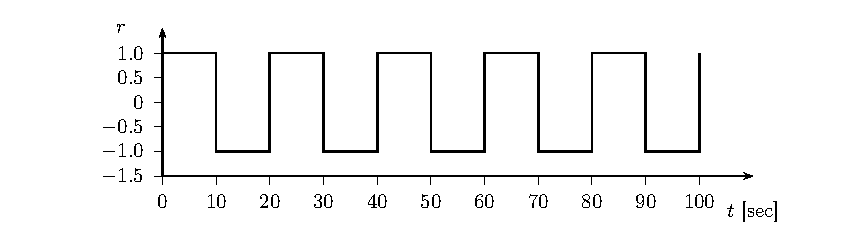
\includegraphics{Obr_cv5Vzor_1.pdf}
	}

    \vspace{-4mm}

	\caption{Referenčný sigál $r$}
	\label{Referenčný sigál $r$ 6cv}

    \vspace{-2mm}

\end{figure}



\begin{figure}[t]
	\centering

	\makebox[\textwidth][c]{%
	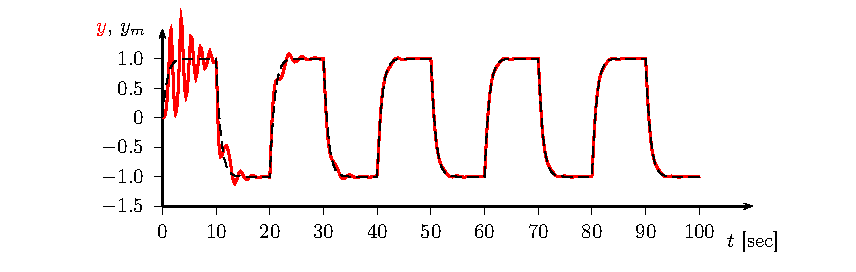
\includegraphics{Obr_cv5Vzor_2.pdf}
	}

    \vspace{-4mm}

	\caption{Výsledok simulácie}
	\label{Výsledok simulácie 6cv}

    \vspace{-2mm}

\end{figure}
















\subsection{Riešenie úloh}



Začiatok úlohy prvej znie:

% \subsubsection{Úloha prvá}



\smallskip

{\color{gray}

Pre nominálnu prenosovú funkciu -- pozri zadanie a riešenie príkladu v časti \ref{pkTMRC} -- pre túto nominálnu prenosovú funkciu riadeného systému navrhnite adaptívne riadenie s~referenčným modelom so vstupno-výstupnou štruktúrou zákona riadenia (merateľný je len výstup riadeného systému a samozrejme vstup). Pre odvodenie zákona adaptácie použite priamu Lyapunovou metódu. Nech referenčný model je v tvare
\begin{equation}
    W_m(s) = \frac{s + 3}{ s^2 + 3.5 s + 3}
\end{equation}

}



% \subsubsection{Bod prvý}
\paragraph{Bod prvý}

\smallskip

{\color{gray}

Určte zákon riadenia, ktorý sa bude používať v adaptívnom riadiacom systéme.

}

\smallskip

\noindent
Viď \eqref{controlLaw}.

Avšak! Hovoríme o \emph{adaptívnom} riadiacom systéme. Prečo sa „adaptujeme“? Pretože nepoznáme hodnoty parametrov riadeného systému. A keďže tieto nepoznáme, nedokážeme vypočítať (ideálne) parametre zákona riadenia, ktorými sú $\Theta_1^\star$, $\Theta_2^\star$, $\Theta_3^\star$ a~$\Theta_4^\star$ (nedokážeme to v „adaptívnom prípade“).

Preto, v adaptívnom riadiacom systéme sa používa zákon riadenia, kde sú ideálne („hviezdičkované“) parametre zákona riadenia nahradené ich odhadmi. Tieto odhady sa „adaptujú“ (priebežne identifikujú) a teda sa menia v čase. Preto píšeme (v~tomto prípade), že adaptovanými parametrami zákona riadenia sú $\Theta_1(t)$, $\Theta_2(t)$, $\Theta_3(t)$ a~$\Theta_4(t)$. Takže v \emph{adaptívnom} riadiacom systéme bude zákon riadenia:
\begin{equation} \label{controlLawAdapt}
	u(t) = \Theta_1(t) \left[ \frac{1}{(s + \lambda)} \right] u(t) + \Theta_2(t) \left[ \frac{1}{(s + \lambda)} \right] y(t) + \Theta_3(t) y(t) + \Theta_4(t) r(t)
\end{equation}











% \subsubsection{Bod druhý}
\paragraph{Bod druhý}

\smallskip

{\color{gray}

Vypočítajte ideálne parametre zákona riadenia.

}

\smallskip

\noindent
Urobili sme tak v časti~\ref{vypocetidealparam}, v Bode druhom.











% \subsubsection{Bod tretí}
\paragraph{Bod tretí}

\smallskip

{\color{gray}

Zistite, či $W_m(s)$ je striktne pozitívne reálna (SPR) prenosová funkcia.

}

\smallskip

\noindent
Máme prenosovú funkciu
\begin{equation}
    W_m(s) = \frac{s + 3}{ s^2 + 3,5 s + 3}
\end{equation}

V prvom bode nás zaujíma, či $W_m(s)$ je reálna pre všetky reálne~$s$. Ak za $s$~dosadíme reálne číslo, potom $W_m(s)$ \emph{je} reálne číslo.

Ďalej nás zaujíma, či menovateľ $W_m(s)$ má korene v~ľavej polrovine komplexnej roviny alebo má reálne korene na imaginárnej osi. Korene polynómu $s^2 + 3,5 s + 3$ sú $s_1 = -2$ a $s_2 = -1,5$. Takže táto podmienka je splnená.

A nakoniec je otázka, či $\Re \left\{ W_m(j\omega) \right\} \geq 0$ pre všetky reálne $\omega$. Vykonajme teda $W_m(s) \to W_m(j\omega)$:
\begin{equation}
    W_m(j\omega) = \frac{j\omega + 3}{ (j\omega)^2 + 3,5 j\omega + 3}
\end{equation}
Toto je (vlastne) nejaké komplexné číslo. Samotná $\omega$ nech je reálne číslo. Upravme.
\begin{subequations}
    \begin{align}
        W_m(j\omega) &= \frac{j\omega + 3}{ (j\omega)^2 + 3,5 j\omega + 3} \\
        &= \frac{j\omega + 3}{ -\omega^2 + 3,5 j\omega + 3} \\
        &= \frac{j\omega + 3}{ \left(3 - \omega^2\right) + j 3,5 \omega }
    \end{align}
\end{subequations}

Je potrebné získať reálnu časť komplexného čísla $W_m(j\omega)$. Pre vyjadrenie reálnej časti je výhodné využiť, že platí:
\begin{equation*}
	\frac{a + jb}{c + jd} = \frac{(a + jb) (c - jd)}{(c + jd) (c - jd)} = \frac{(a + jb) (c - jd)}{c^2 + d^2}
\end{equation*}
Takže:
\begin{subequations}
    \begin{align}
        W_m(j\omega) &=
        \frac{ \left( j\omega + 3 \right)}{ \left( \left(3 - \omega^2\right) + j 3,5 \omega \right) }
        \frac{ \left( \left(3 - \omega^2\right) - j 3,5 \omega \right)}{ \left( \left(3 - \omega^2\right) - j 3,5 \omega \right) }
        \\ & =
        \frac{ \left( j\omega + 3 \right) \left( \left(3 - \omega^2\right) - j 3,5 \omega \right)}{ \left(3 - \omega^2\right)^2 + \left(3,5 \omega \right)^2 }
        \\ & =
        \frac{ 9 - 3 \omega^2 - j 10,5 \omega + j 3 \omega - j \omega^3 + 3,5 \omega^2  }{ \left(3 - \omega^2\right)^2 + \left(3,5 \omega \right)^2 }
    \end{align}
\end{subequations}
Reálna časť z toho je
\begin{align}
    \Re \left\{ W_m(j\omega) \right\}
    & =
    \frac{ 9 + 0,5 \omega^2 }{ \left(3 - \omega^2\right)^2 + \left(3,5 \omega \right)^2 }
\end{align}
a teda platí $\Re \left\{ W_m(j\omega) \right\} \geq 0 \  \forall \  \omega \in \mathbb R$.
Prenosová funkcia $W_m(s)$ je SPR.









% \subsubsection{Bod štvrtý}
\paragraph{Bod štvrtý}

\smallskip

{\color{gray}

Napíšte rovnicu výstupnej adaptačnej odchýlky $e_1$.

}

\smallskip

\noindent
Výstupná adaptačná odchýlka je, samozrejme, $e_1(t) = y(t) - y_m(t)$. Tu sa však myslí písanie rovnice, ktorá opisuje dynamiku adaptačnej odchýlky. Teda
\begin{equation} \label{vvMRAC_adaptOdchDefTFt}
	e_1(t) =  \left[ W_m(s)  \right] \frac{1}{\Theta_4^\star} \left( \theta^\naT(t) \ \omega(t) \right)
\end{equation}
kde pre podrobný význam jednotlivých symbolov odkazujeme čitateľa na študijný materiál k príslušnej téme. V skratke, je jasné, že $W_m(s)$ je prenosová funkcia referenčného modelu, $\Theta_4^\star$ je jeden y ideálnych parametrov zákona riadenia, $\theta^\naT(t)$ je vektor pozostávajúci z odchýlok medzi ideálnymi parametrami zákona riadenia a~ich odhadmi a~$\omega(t)$ je signálny vektor zákona riadenia.

Mimochodom, toto je veľmi veľmi dôležitá rovnica celkovo v oblasti akejkoľvek priebežnej identifikácie parametrov (alebo adaptácie ak chcete). Podrobnosti sú ďaleko nad rámec tohto textu\ldots














% \subsubsection{Bod piaty}
\paragraph{Bod piaty}

\smallskip

{\color{gray}

Pre systém diferenciálnych rovníc ($\dot e$, $\dot \theta$), kde $\dot \theta$ sa najskôr uvažuje vo všeobecnom tvare (na začiatku odvodenia sa uvažuje len všeob. funkcia $f$) zvoľte kandidáta na Lyapunovovu funkciu a odvoďte (skonkretizujte) predpis (pravú stranu) pre $\dot \theta$.

}

\smallskip

\noindent
Ako je čitateľovi iste známe, rovnicu opisujúcu dynamiku adaptačnej odchýlky je možné zapísať aj pomocou nejakého stavového vektora, konkrétne sa v učebnom texte uvádza
\begin{subequations} \label{vvMRAC_adaptOdchDefSSt}
	\begin{align}
		\dot e(t) &= A_c e(t) + \overline{B}_c \frac{1}{\Theta_4^\star} \left( \theta^\naT(t) \omega(t) \right) \\
		e_1(t) &= C_c^\naT e(t)
	\end{align}
\end{subequations}
pričom $W_m(s) = C_c^\naT \left( s I - A_c \right)^{-1} \overline{B}_c$ a pre ďalšie podrobnosti viď príslušný učebný text.

Tu vieme, čo je signál $e_1(t)$ a aj ho vieme merať/získať. Vonkoncom nevieme merať/získať stavový vektor $e(t)$. Ale vieme, že existuje. Teoreticky.

Nič nebráni zostaveniu systému diferenciálny rovníc v tvare
\begin{subequations} \label{zossysdifr}
	\begin{align}
		\dot e(t) &= A_c e(t) + \overline{B}_c \frac{1}{\Theta_4^\star} \left( \theta^\naT(t) \omega(t) \right) \\
		\dot \theta(t) &= f(e_1(t), \omega(t))
	\end{align}
\end{subequations}
a tento systém má, ako je uvedené v učebnom texte, veľmi výhodné vlastnosti vzhľadom na možnosti adaptácie (priebežnej identifikácie) pre dosiahnutie cieľa riadenia.

Inými slovami, ak systém diferenciálnych rovníc \eqref{zossysdifr} bude stabilný (plus pár miliónov detailov detailov), tak stavový vektor $e(t)$ sa bude asymptoticky (s časom) blížiť k nule. Je potom jasné, že aj adaptačná odchýlka $e_1(t)$ sa bude blížiť k nule, čo je cieľ riadenia. Podrobnosti prečo to tak je, sa najlepšie ukazujú na prípade MRAC stavového (ako sme spomenuli v jednom odstavci vyššie - v časti~\ref{cast1bodtreti}, v Bode treťom).

Jasným (viac-menej) kandidátom na Lyapunovovu funkciu pre systém \eqref{zossysdifr} teda je (si dovolíme nepísať signály ako funkcie času, teda napr. píšeme len $e$ nie $e(t)$)
\begin{equation}
	V = e^\naT P e + \left| \frac{1}{\Theta_4^\star} \right| \theta^\naT \Gamma^{-1} \theta
\end{equation}

Cesta potom vedie do bodu, kde máme
\begin{align} \label{dolbod}
	\dot{V} &= e^\naT \left( - Q \right) e + 2 \left( e^\naT P \overline{B}_c \right) \frac{1}{\Theta_4^\star} \theta^\naT \omega + 2 \left| \frac{1}{\Theta_4^\star} \right| \theta^\naT \Gamma^{-1} \dot{\theta}
\end{align}
a chceme zabezpečiť aby časová derivácia $\dot{V}$ bola záporne definitná. Na pravej strane rovnice \eqref{dolbod}, člen $e^\naT \left( - Q \right) e$ je záporne definitný (vždy menší ako nula). Ak by na pravej strane rovnice \eqref{dolbod} zvyšné dva členy neboli platilo by požadované $\dot{V} \leq 0$. Inými slovami žiadame:
\begin{subequations}
	\begin{align}
    	0 &= 2 \left( e^\naT P \overline{B}_c \right) \frac{1}{\Theta_4^\star} \theta^\naT \omega + 2 \left| \frac{1}{\Theta_4^\star} \right| \theta^\naT \Gamma^{-1} \dot{\theta} \\
    	2 \left| \frac{1}{\Theta_4^\star} \right| \theta^\naT G^{-1} \dot{\theta} &= - 2 \left( e^\naT P \overline{B}_c \right) \frac{1}{\Theta_4^\star} \Theta^\naT \omega \\
    	\left| \frac{1}{\Theta_4^\star} \right| \Gamma^{-1} \dot{\theta} &= - \left( e^\naT P \overline{B}_c \right) \, \texttt{sign}\left(\frac{1}{\Theta_4^\star}\right) \left| \frac{1}{\Theta_4^\star} \right| \omega \\
    	\Gamma^{-1} \dot{\theta} &= - \texttt{sign}\left(\frac{1}{\Theta_4^\star}\right) \left( e^\naT P \overline{B}_c \right) \omega \\
    	\dot{\theta} &= - \texttt{sign}\left(\frac{1}{\Theta_4^\star}\right) \left( e^\naT P \overline{B}_c \right) \Gamma \omega
	\end{align}
\end{subequations}

Tu sme, v princípe, práve získali hľadaný zákon adaptácie, teda predpis, ktorý hovorí ako sa mení vektor $\theta$. Avšak, obsahuje vektor $e$. Ten nemáme. Všetko uvedené je len teoretické.

Tu sa využije veľmi významná vlastnosť, že prenosová funkcia $W_m(s)$ je SPR. Pripomeňme, že pre ňu platí $W_m(s) = C_c^\naT \left( s I - A_c \right)^{-1} \overline{B}_c$ a s využitím tejto reprezentácie referenčného modelu je možné využiť Meyerovu-Kalmanovu-Yakubovichovu Lemmu (vetu). Podľa nej platí
\begin{align*}
	  A_c^\naT P + P A_c &= - Q\\
	  P \overline{B}_c &= C_c
\end{align*}
kde by sme mali byť oboznámený čo konkrétne teraz sú uvedené matice\ldots

Keďže platí $P \overline{B}_c = {C_c}$, tak máme
\begin{subequations}
	\begin{align}
        \dot{\theta} &= - \texttt{sign}\left(\frac{1}{\Theta_4^\star}\right) \left( e^\naT P \overline{B}_c \right) \Gamma \omega \\
    	\dot{\theta} &= - \texttt{sign}\left(\frac{1}{\Theta_4^\star}\right) \left( e^\naT C_c \right) \Gamma \omega
	\end{align}
\end{subequations}
Výraz $e^\naT C_c$ je skalár. Takže $e^\naT C_c = C_c^\naT e$. A potom je jasné, že $C_c^\naT e = e_1$. Preto môžeme písať
% \begin{subequations}
	\begin{align}
    	\dot{\theta} &= - \texttt{sign}\left(\frac{1}{\Theta_4^\star}\right) e_1 \Gamma \omega
	\end{align}
% \end{subequations}
Toto je stále hľadaný zákon adaptácie. Ale už neobsahuje nedostupný (len teoretický) vektor $e$ ale dostupný signál $e_1$, čo je jednoducho výstupná adaptačná odchýlka.












% \subsubsection{Bod šiesty}

\paragraph{Bod šiesty}

\smallskip

{\color{gray}

Určte zákon adaptácie, ktorý sa bude používať v adaptívnom riadiacom systéme.

}

\smallskip

\noindent
Práve sme tak urobili v predchádzajúcom bode. Zákon adaptácie je
\begin{align}
    \dot \Theta(t) &= - \texttt{sign}\left(\frac{1}{\Theta_4^\star}\right) e_1(t)\ \Gamma\ \omega(t)
\end{align}

Pripomeňme, že signálny vektor zákona riadenia v tomto prípade je
\begin{align}
    \omega(t) =
    \begin{bmatrix}
          y(t) \\ \nu_1(t) \\ \nu_2(t) \\  r(t)
    \end{bmatrix}
\end{align}
takže zákon adaptácie detailnejšie napísaný je
\begin{align}
    \dot \Theta(t) &=
    - \texttt{sign}\left(\frac{1}{\Theta_4^\star}\right)
    e_1(t)
    \begin{bmatrix}
        \gamma_1 & 0 & 0 & 0 \\
        0 & \gamma_2 & 0 & 0 \\
        0 & 0 & \gamma_3 & 0 \\
        0 & 0 & 0 & \gamma_4
    \end{bmatrix}
    \begin{bmatrix}
          y(t) \\ \nu_1(t) \\ \nu_2(t) \\  r(t)
    \end{bmatrix}
\end{align}
kde sme ako príklad zvolili maticu $\Gamma$ diagonalnu s kladnými číslami $\gamma_1, \cdots, \gamma_4$ na diagonále.



















% \subsubsection{Bod siedmi}

\paragraph{Bod siedmi}

\smallskip

{\color{gray}

Zvoľte $\Gamma$ (jednoducho, zvoľte všetky ľubovolne voliteľné prvky zákona/zákonov adaptácie).

}

\smallskip

\noindent
Voľba matice $\Gamma$ ako diagonálnej matice v prvom rade spĺňa podmienky pre túto maticu (má byť symetrická a kladne definitná). Má to však aj praktický význam. Matica  $\Gamma$ je hlavným nástrojom ako ovplyvniť vlastnosť zákona adaptácie, ktorá sa nazýva rýchlosť adaptácie. Ak je navyše diagonálna, vieme relatívne nezávisle ovplyvňovať rýchlosť adaptácie jednotlivých prvkov vektora adaptovaných parametrov. Uvažujme teda o matici $\Gamma$ v tvare
\begin{align}
    \Gamma =
    \begin{bmatrix}
        \gamma_1 & 0 & 0 & 0 \\
        0 & \gamma_2 & 0 & 0 \\
        0 & 0 & \gamma_3 & 0 \\
        0 & 0 & 0 & \gamma_4
    \end{bmatrix}
\end{align}

V tomto prípade máme vektor adaptovaných parametrov v tvare
\begin{align}
    \Theta(t) =
    \begin{bmatrix}
          \Theta_3(t) \\ \Theta_1(t) \\ \Theta_2(t) \\ \Theta_4(t)
    \end{bmatrix}
\end{align}
Ak by sme chceli ovplyvniť rýchlosť s akou sa mení napr. parameter $\Theta_2(t)$, je to možné urobiť zmenou veľkosti čísla $\gamma_3$ v matici $\Gamma$. Ak zvýšime $\gamma_3$, potom $\dot \Theta_2(t)$ bude dosahovať v princípe vyššie hodnoty, a naopak\ldots














% \subsubsection{Bod ôsmy až desiaty}

\paragraph{Bod ôsmy až desiaty}

\smallskip

{\color{gray}

\begin{itemize}[leftmargin=0pt, labelsep=4mm, itemsep=0pt]
    \item Začiatočné hodnoty adaptovaných parametrov zvoľte nulové.
    \item Zostavte adaptívny riadiaci systém (simulačnú schému) a pridajte ho k~simulovanej sústave.
    \item Použite obdĺžnikový referenčný signál $r$ ako na Obr.~\ref{Referenčný sigál $r$ 6cv}. Vzorové výsledky simulácie sú na Obr.~\ref{Výsledok simulácie 6cv}.
\end{itemize}

}

\smallskip










\noindent
Nasledujúci výpis kódu~\ref{vypk07} obsahuje funkciu \lstinline|fcn_simSch3|. Je postavená na rovnakých princípoch ako sme tu už viac krát uviedli. Rozdielom oproti predchádzajúcej simulácii vo výpise kódu~\ref{vypk06} je pridanie zákona adaptácie (nahradenie pevne stanovených hodnôt vektora \lstinline|Theta|).

Výsledky simulácie pre uvedené zadanie sú na obr.~\ref{figsc_ar06_MRAC_1}.


\begin{figure}[t]
	\centering

	\makebox[\textwidth][c]{%
	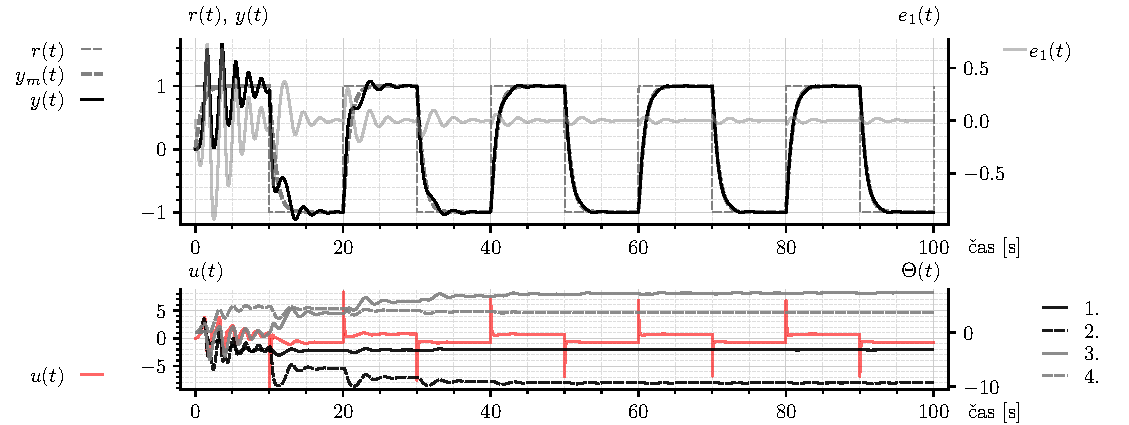
\includegraphics{figsc_ar06_MRAC_1.pdf}
	}

    \vspace{-2mm}

	\caption{Výsledok simulácie}
	\label{figsc_ar06_MRAC_1}


    \vspace{-2mm}

\end{figure}






{\catcode`\-=12
\lstinputlisting[language=Python,
                 caption={Súbor \lstinline{ar06_prMRAC_v01.py}, simulačná schéma adaptívneho riadiaceho systému},
                 label={vypk07},
				 consecutivenumbers=false,
				 linerange=c01-c01,
                 ]{../../PY/ar06_prMRAC_v01.py}
}






\subsection{Dodatok k riešeniu (prevažne o nastavovaní rýchlosti adaptácie)}


Vo svetle toho, že v tomto príklade je použitý model reálneho systému -- jednosmerného motora, uvažujme realistickejšiu simuláciu. Zmysluplné okolie pracovného bodu je $\pm 0,7$ [V], teda má význam žiadať od výstupnej veličiny $y(t)$ maximálne hodnoty $\pm 0,7$ a akčný zásah môže byť v rozsahu cca $\pm 5$ (tiež vo voltoch, ale to sú už prílišné podrobnosti keďže čitateľ zrejme nepozná detaily k riadenému systému).














\paragraph{Prípad 1}



Preto, použime rovnaké nastavenie adaptívneho riadiaceho systému ako vo „vzorovej“ (umelo vymyslenej) simulácii a v prvom rade zmeňme priebej referenčného signálu. Výsledok je na obr.~\ref{figsc_ar06_MRAC_2}.




Priebeh veličín riadeného systému, vústupnej aj vstupnej, je v poriadku z hľadiska rozsahov (v okolí pracovných bodov to zodpovedá reálnemu systému (motorčeku)). Povedzme však, že rýchlosť adaptácie (výsledok na obr.~\ref{figsc_ar06_MRAC_2}) je nevyhovujúca. Nech je požiadavka taká, že v čase 100 má byť riadiaci systém už adaptovaný. Je teda potrebné upraviť voliteľný parameter zákona adaptácie, ktorý vo veľkej miere určuje rýchlosť adaptácie. Tým ja matica $\Gamma$. V tomto „vzorovom“ prípade vidíme, že sa uvažuje
\begin{lstlisting}[language=Python,
                    numbers=none,
                    ]
Gamma = np.diag(np.array([5, 50, 50, 5]))
\end{lstlisting}












\begin{figure}[!t]
	\centering

    \vspace{-3mm}

	\makebox[\textwidth][c]{%
	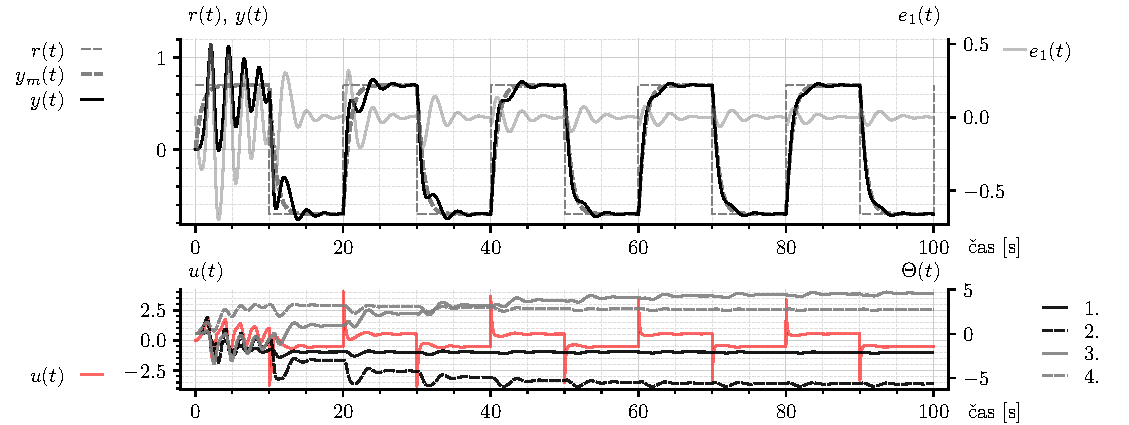
\includegraphics{figsc_ar06_MRAC_2.pdf}
	}

    \vspace{-2mm}

	\caption{}
	\label{figsc_ar06_MRAC_2}


    \vspace{-2mm}

\end{figure}






\paragraph{Prípad 2}

Výslednú rýchlosť adaptácie však neovplyvňuje len matica $\Gamma$ ale samozrejme všetky prvky v zákone adaptácie. Teda signálny vektor $\omega$ a samozrejme adaptačná odchýlka. Všetky tieto signály - ich charakter a vplyv na rýchlosť adaptácie, závisia od toho ako veľmi tzv. \emph{vybudíme} systém\footnote{Tu si dovolíme smerovať čitateľa na pojem \emph{persistent excitation} v adaptívnych systémoch alebo pri priebežnej identifikácii vo všeobecnosti \#UTFG \#nooffense.}.


Pod vybudením sa mysllí navodenie takých podmienok, aby sa prejavili takpovediac všetky vlastnosti systému. V tu uvažovanej schéme je viac menej jedinou možnosťou ako „vybudiť“ riadený systém je riadiť ho tak, že sledujeme relatívne „zložitý“ referenčný signál. Naopak, ak referenčný signál je „jednoduchý“, tak je ho aj jednoduché sledovať, a takpovediac blok adaptácie ľahko nájde vhodné parametre zákona riadenia (tak aby $y(t)$ sledovalo $y_m(t)$)\footnote{Mimochodom, referenčný signál by sme si v praxi pravdepodobne nemohli len tak zvoliť, ak, tak azda pre „fázu učenia/adaptácie“ a podobne. Aj toto treba mať na pamäti pri uvažovaní o~tu uvedených poznámkach.}.

Jednoduchým (v princípe najjdednoduchším) referenčným signálom je sínusoida („obsahuje“ len jednu frekvenciu, obdĺžnikový signál „obsahuje“ nekonečne veľa frekvencií). Vyskúšakme teda $r(t)$ ako harmonický signál s periódou 20 [časových jednotiek - sekúnd v realite] a amplitúdou 0,7 [voltov v realite]. Pritom pre začiatok uvažujme
\begin{lstlisting}[language=Python,
                    numbers=none,
                    ]
Gamma = np.diag(np.array([1, 1, 1, 1]))
\end{lstlisting}
Výsledok je na obr.~\ref{figsc_ar06_MRAC_3}. Adaptačná odchýlka sa s časom  zmenšuje, ale povedzme, že nie dostatočne rýchlo.






\begin{figure}[!b]
	\centering

    \vspace{-3mm}

	\makebox[\textwidth][c]{%
	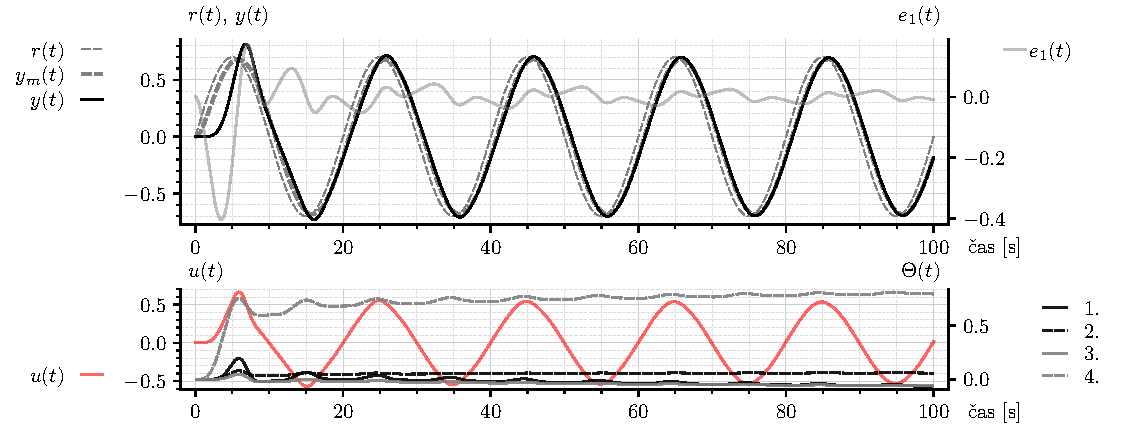
\includegraphics{figsc_ar06_MRAC_3.pdf}
	}

    \vspace{-2mm}

	\caption{}
	\label{figsc_ar06_MRAC_3}


    \vspace{-2mm}

\end{figure}















\paragraph{Prípad 3}

Na priebehu adaptovaných parametrov (vektor $\Theta(t)$) je vidieť, že najrýchlejšie zmeny boli pri parametri $\Theta_4$. Skúsme docieliť, aby sa aj ostatné parametre menili rýchlejšie - prípadne, aby sa parameter $\Theta_4$ menil pomalšie. Jednoducho, aby adaptácia všetkých parametrov prebiehala „relatívne rovnako rýchlo“.

S pomocou cieľavedomého experimentovania a kvalifikovaného odhadu\footnote{Nie, na toto neexistuje univerzálny návod.} sme, dajme tomu, dospeli k nasledujúcim hodnotám v matici $\Gamma$:
\begin{lstlisting}[language=Python,
                    numbers=none,
                    ]
Gamma = np.diag(np.array([3, 5, 10, 0.5]))
\end{lstlisting}
Výsledok je na obr.~\ref{figsc_ar06_MRAC_4}. Je možné konštatovať, že všetky parametre sa menili (na začiatku určite) rovnako rýchlo. Celková rýchlosť zmenšovania sa adaptačnej odchýlky je však pri tom relatívne rovnaká ako v predchádzajúvom prípade.





\begin{figure}[!t]
	\centering

    \vspace{-3mm}

	\makebox[\textwidth][c]{%
	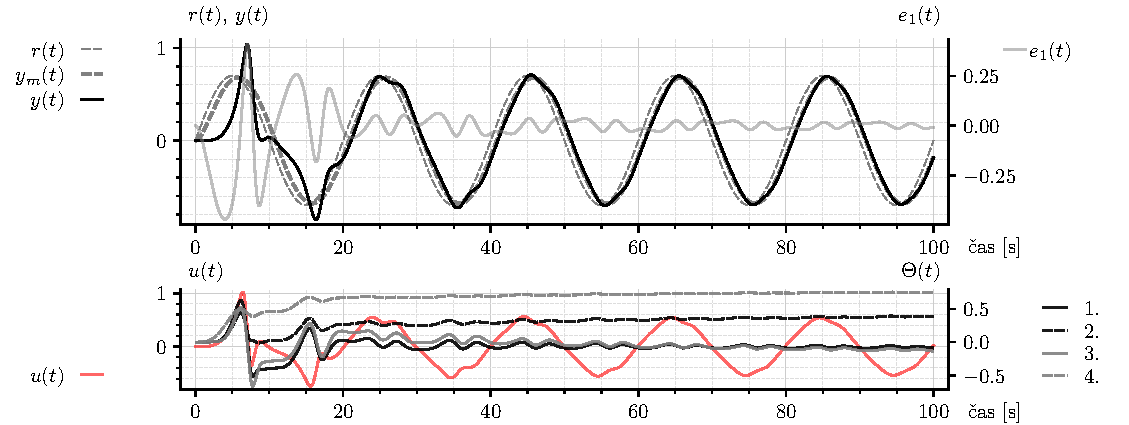
\includegraphics{figsc_ar06_MRAC_4.pdf}
	}

    \vspace{-2mm}

	\caption{}
	\label{figsc_ar06_MRAC_4}


    \vspace{-2mm}

\end{figure}









\paragraph{Prípad 4}

Ak by sme teraz chceli zvýšiť celkovú rýchlosť adaptácie, je možné urobiť napr.:
\begin{lstlisting}[language=Python,
                    numbers=none,
                    ]
Gamma = np.diag(np.array([3, 5, 10, 0.5])*2)
\end{lstlisting}
Výsledok je na obr.~\ref{figsc_ar06_MRAC_5}.






\begin{figure}[!b]
	\centering

    \vspace{-3mm}

	\makebox[\textwidth][c]{%
	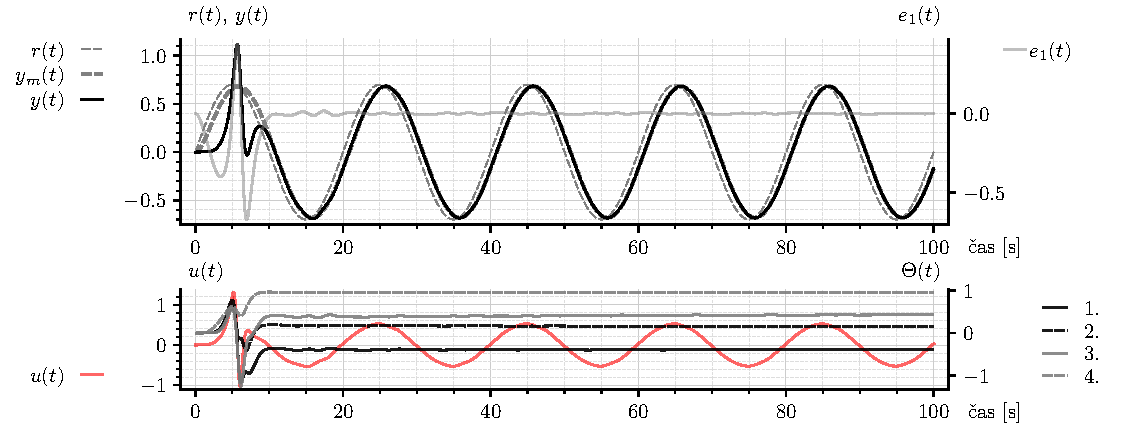
\includegraphics{figsc_ar06_MRAC_5.pdf}
	}

    \vspace{-2mm}

	\caption{}
	\label{figsc_ar06_MRAC_5}


    \vspace{-2mm}

\end{figure}








\paragraph{Prípad 5}

Vyskúšajme s touto voľbou $\Gamma$ zložitejší referenčný signál ako v prípade 1. Výsledok je na obr.~\ref{figsc_ar06_MRAC_6}. Rýchlosť zmeny jednotlivých adaptovaných parametrov je relatívne rovnaká, avšak celková rýchlosť adaptácie nie je dostatočná.








\paragraph{Prípad 6}

Preto:
\begin{lstlisting}[language=Python,
                   numbers=none,
                    ]
Gamma = np.diag(np.array([3, 5, 10, 0.5])*10)
\end{lstlisting}
Výsledok je na obr.~\ref{figsc_ar06_MRAC_7}. Rýchlosť adaptácie sme jednoznačne zvýšili a mohli by sme ju zvyšovať aj viac.







\paragraph{Prípad 7}

Všimnime si ale, že sme uvažovali signál $r(t)$ len v kladných hodnotách. „Nevybudili“ sme systém v celom potenciálnom rozsahu okolia pracovného bodu. Skúsme preto ponechať aktuálne nastavenie $\Gamma$ ale zmeniť $r(t)$ - viď obr.~\ref{figsc_ar06_MRAC_8}.



Zmena $r(t)$, v zmysle, že je viac „budiaci“,  sa jednoznačne prejavila v rýchlosti ustálenia sa adaptovaných parametrov a mierne aj na rýchlosti zmenšovania sa adaptačnej odchýlky.









\begin{figure}[!t]
	\centering

    \vspace{-3mm}

	\makebox[\textwidth][c]{%
	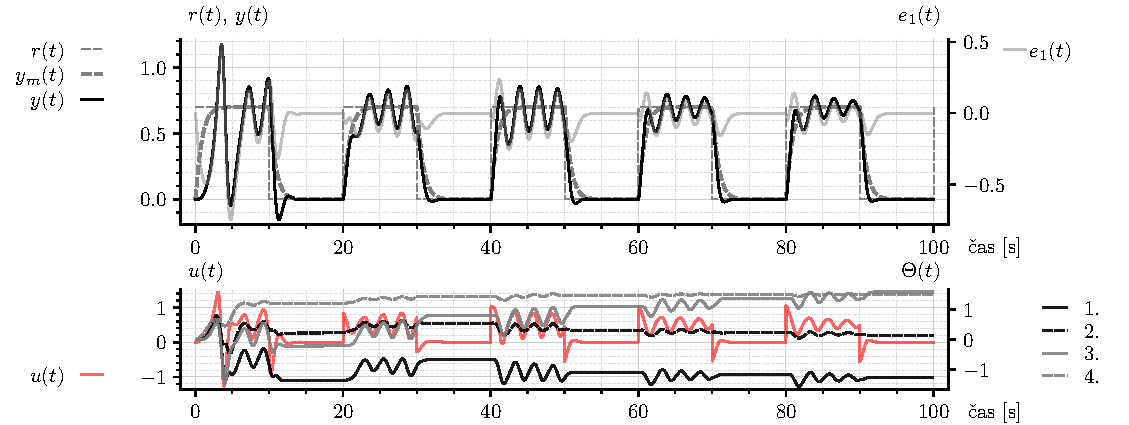
\includegraphics{figsc_ar06_MRAC_6.pdf}
	}

    \vspace{-2mm}

	\caption{}
	\label{figsc_ar06_MRAC_6}


    \vspace{-2mm}

\end{figure}








\begin{figure}[!b]
	\centering

    \vspace{-3mm}

	\makebox[\textwidth][c]{%
	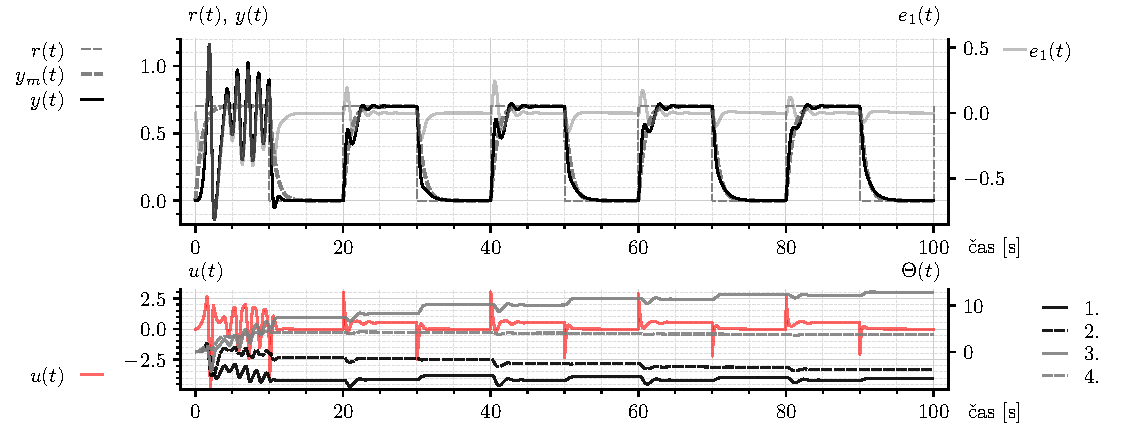
\includegraphics{figsc_ar06_MRAC_7.pdf}
	}

    \vspace{-2mm}

	\caption{}
	\label{figsc_ar06_MRAC_7}


    \vspace{-2mm}

\end{figure}











\begin{figure}[!t]
	\centering

    \vspace{-3mm}



	\makebox[\textwidth][c]{%
	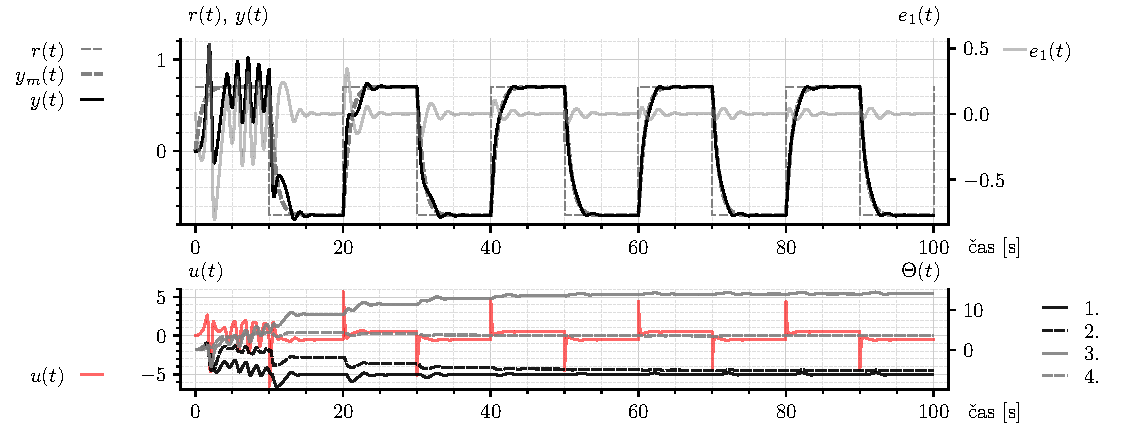
\includegraphics{figsc_ar06_MRAC_8.pdf}
	}

    \vspace{-2mm}

	\caption{}
	\label{figsc_ar06_MRAC_8}


    \vspace{-2mm}

\end{figure}































\section{Príklad k téme \emph{Zákon adaptácie pri $n^* = 2$}}


V predchádzajúcom príklade sme sa zaoberali prípadom, keď model riadeného systému bola prenosová funkcia, ktorej relatívny stupeň bol $n^* = 1$. V tejto časti je príklad, keď riadený systém má význam modelovať prenosovou funkciou s relatívnym stupňom $n^* = 2$.








\subsection{Celkový pohľad na úlohu}


Nech riadeným systémom je kyvadlo a nech riadenou veličinou je poloha (uhol) kyvadla. Zároveň, nech riadený systém je daný diferenciálnou rovnicou opisujúcu dynamiku rotačného pohybu kyvadla. Rovnica je v tvare
\begin{equation} \label{analOpRS}
    ml^2 \ddot{\varphi}(t) + \beta \dot{\varphi}(t) + mgl\sin{\varphi(t)} = u(t)
\end{equation}
kde hmotný bod s hmotnosťou $m$ [kg] pripevnený na ramene so zanedbateľnou hmotnosťou a dĺžkou $l$ [m] kmitá (otáča sa okolo osi). Kmity sú tlmené viskóznym trením s koeficientom $\beta$ [kg m$^2$ s$^{-1}$]. Uhol medzi zvislicou a ramenom kyvadla je označený $\varphi$ [rad] a gravitačné zrýchlenie je $g = 9,81$ [m s$^{-2}$]. Signál $u(t)$ [kg m$^2$ s$^{-2}$] je externý moment sily pôsobiaci na rameno kyvadla, $\dot{\varphi}(t)$ [rad s$^{-1}$] je uhlová rýchlosť a $\ddot{\varphi}(t)$ [rad s$^{-2}$] je uhlové zrýchlenie ramena kyvadla.
Číselné hodnoty parametrov kyvadla sú nasledovné:
\begin{align*}
	m &= 1 \quad \text{[kg]}\\
	l &= 1 \quad \text{[m]}\\
	\beta &= 2 \cdot 0,5 \cdot \sqrt{\frac{g}{l}} \quad \text{[kg m$^2$ s$^{-1}$]}
\end{align*}

Cieľom je riadiť polohu kyvadla v okolí rôznych pracovných bodov. Uvažujme však, že pracovné body sú z intervalu polôh kyvadla 0 až 90 stupňov. Konkrétna voľba pracovných bodov ako aj voľba veľkosti ich okolia sa ponechávajú na čitateľa.

Nech dynamika výstupnej veličiny riadeného systému v ktoromkoľvek pracovnom bode je daná referenčným modelom, ktorým je lineárny dynamický systém s pólmi $p_1 = -2$ a $p_2 = -1$. Samozrejmé je, že tento lineárny dynamický systém bude mať jendnotkové statické zosilnenie.

\paragraph{Referenčný model}

Ak vieme, že RM je druhého rádu, a tiež vlastne vieme (aj keď sme to ešte explicitne neukázali), že sa zaoberáme riadeným systémom, ktorého (lineárny) model má relatívny stupeň $n^* = 2$, potom z toho plynie, že referenčný model má tvar
\begin{equation}
    W_m(s) = \frac{2}{ s^2 + 3 s + 2}
\end{equation}








\subsubsection{Celkový pohľad na riadený systém (z hľadiska návrhu riadiaceho systému)}

Pre lepšiu predstavu o riadenom systéme ho opíšme v stavovom priestore. Voľbou stavových veličín $x_1(t) = \varphi(t)$ a~$x_2(t) = \dot\varphi(t)$ máme
\begin{subequations} \label{stavopnonlinkyv}
	\begin{align}
		\begin{bmatrix}
			\dot{x}_1(t) \\ \dot{x}_2(t)
		\end{bmatrix}
		&=
		\begin{bmatrix}
			x_2(t) \\ - \frac{\beta}{ml^2} x_2(t) - \frac{g}{l} \sin\left(x_1(t)\right)
		\end{bmatrix}
		+
		\begin{bmatrix}
			0 \\ \frac{1}{ml^2}
		\end{bmatrix}
		u(t) \\
		y(t) &= x_1(t)
	\end{align}
\end{subequations}
kde sme pre prehľadnosť v nasledujúcom zaviedli aj výstupnú veličinu $y(t) = \varphi(t)$.


Toto je, zjavne, nelineárny časovo-invariantný systém druhého rádu. Tu sa však zaoberáme takou triedou riadiacich systémov, ktoré predpokladajú lineárny model riadeného systému. Jeho parametre môžu byť neznáme (môžu sa meniť), ale musí byť lineárny.

\paragraph{Linearizácia v okolí pracovného bodu}

Uvažovaný riadený systém je možné linearizovať v okolí pracovného bodu.

V prvom rade potrebujeme poznať pracovný bod. Pre zvolenú hodnotu (ustálenú) na vstupe systému, označme ju $u_{PB}$, potrebujeme poznať prislúchajúcu hodnotu (ustálenú) na výstupe, označme ju $y_{PB}$.

Tu máme k dispozícii analytický opis riadeného systému \eqref{analOpRS}. V ustálenom stave (časové derivácie nulové) máme
\begin{subequations}
    \begin{align}
        \left(m g l\right)\sin\left(y_{PB}\right) &= u_{PB} \\
         y_{PB} &= \arcsin \left( \frac{1}{ \left(m g l\right)} u_{PB} \right)
    \end{align}
\end{subequations}
Toto je, samozrejme, prevodová charakteristika riadeného systému. Nie je to priamka. To znamená, že v jednom pracovnom bode (v okolí jedného pracovného bodu) bude statické zosilnenie (sklon prevodovej charakteristiky) iné, ako v inom pracovnom bode (v okolí iného pracovného bodu).

\bigskip

Mimochodom, zvoľme si veľkosť okolia pracovného bodu. Dobrou pomôckou je grafické zobrazenie prevodovej charakteristiky. To sa ponecháva na čitateľa (autor je lenivý). Tu si zvoľme okolie z veľkosťou $\pm 3$ [°] (cca $0,0524$ [rad]) na strane výstupnej veličiny a~buďme s ním spokojný v tom zmysle, že pri takýchto malých odchýlkach si prevodová charakteristika zachováva prakticky rovnaký sklon ako v pracovnom bode.

\bigskip

Ďalej je potrebné zaviesť veličiny, ktoré budú takpovediac odchýlkami odhodnôt v pracovnom bode. Konkrétne
\begin{subequations}
    \begin{align}
        \Delta u(t) &= u(t) - u_{PB} \\
        \Delta y(t) &= y(t) - y_{PB}
    \end{align}
\end{subequations}
kde sme teta definovali $\Delta$ odchýlky od pracovného bodu. To znamená, že pôvodné veličiny sú
\begin{subequations}
    \begin{align}
        u(t)  &=  u_{PB} + \Delta u(t) \\
        y(t)  &=  y_{PB} + \Delta y(t) \\
        x_1(t)  &=  x_{1PB} + \Delta x_1(t) \\
        x_2(t)  &=  x_{2PB} + \Delta x_2(t)
    \end{align}
\end{subequations}
kde sme rovnako yaviedli „odchýlkové veličiny“ aj pre stavové veličiny so systému \eqref{stavopnonlinkyv}. Dosaďme v \eqref{stavopnonlinkyv}, čo v prvom rade znamená, že
% \begin{subequations}
	\begin{align}
		\begin{bmatrix}
			\frac{\text{d}}{\text{d}t} \left( x_{1PB} + \Delta x_1(t) \right)   \\
            \frac{\text{d}}{\text{d}t} \left( x_{2PB} + \Delta x_2(t) \right)
		\end{bmatrix}
        =
        \begin{bmatrix}
			 \Delta \dot x_1(t)    \\
             \Delta \dot x_2(t)
		\end{bmatrix}
	\end{align}
% \end{subequations}
pretože $x_{1PB}$ a $x_{2PB}$ su len čísla nezávislé od času. Potom na základe \eqref{stavopnonlinkyv} môžme písať



\begin{subequations} \label{stavopnonlinkyv2}
	\begin{align}
        \Delta \dot x_1(t) &= \left( x_{2PB} + \Delta x_2(t) \right) \\
        \Delta \dot x_2(t) &=
        - \frac{\beta}{ml^2} \left( x_{2PB} + \Delta x_2(t) \right) - \frac{g}{l} \sin\left( \left( x_{1PB} + \Delta x_1(t) \right) \right)
        + \frac{1}{ml^2} \left( u_{PB} + \Delta u(t) \right) \\
        \Delta y(t) &= \Delta x_1(t)
	\end{align}
\end{subequations}
kde sme zohľadnili, že musi platiť $\Delta y(t) = \Delta x_1(t)$, keďže máme $y(t) = x_1(t)$. Rovnice \eqref{stavopnonlinkyv2} opisujú stále to isté nelineárne kyvadlo, avšak pomocou iných („odchýlkových“) veličín. Je to užitočné preto, že tento „nový“ systém má ustálený stav $x_e$ (ekvilibrium) v bode
\begin{align}
    x_e =
    \begin{bmatrix}
        \Delta x_{e1}    \\
        \Delta x_{e2}
    \end{bmatrix}
    =
    \begin{bmatrix}
        0    \\
        0
    \end{bmatrix}
\end{align}
a to samozrejme pri $\Delta u(t) = 0$. V tomto „novom“ ustálenom stave, očividne, pre pôvodné veličiny platí, že $u(t)  =  u_{PB}$ a $y(t)  =  y_{PB}$. Teda systém je ustálený v pracovnom bode. V tomto „novom“ ekvilibriu, je možné systém štandardne linearizovať. Výsledkom je
\begin{subequations} \label{stavoplinkyv}
    \begin{align}
    	\begin{bmatrix}
        	  \Delta \dot x_1(t) \\
    		  \Delta \dot x_2(t)
     	\end{bmatrix}
    	&=
    	\begin{bmatrix}
        	0 & 1 \\
        	- \frac{g}{l} \cos \left( y_{PB} \right) & - \frac{\beta}{m\ l^2}
      	\end{bmatrix}
        \begin{bmatrix}
        	  \Delta x_1(t) \\
    		  \Delta x_2(t)
     	\end{bmatrix}
        +
        \begin{bmatrix}
        	  0 \\
    		  \frac{1}{m\ l^2}
     	\end{bmatrix}
        \Delta u(t)
        \\
        \Delta y(t)
        &=
        \begin{bmatrix}
            1 & 0 \\
        \end{bmatrix}
        \begin{bmatrix}
              \Delta x_1(t) \\
              \Delta x_2(t)
        \end{bmatrix}
    \end{align}
\end{subequations}


Toto je lineárny dynamický systém, ktorý je možné zapísať v tvare prenosovej funkcie
\begin{align}
    \frac{\Delta y(s)}{\Delta u(s)} = \frac{k_p}{s^2 + a_1 s + a_0}
\end{align}
kde
\begin{subequations}
    \begin{align}
        k_p &= \frac{1}{m\ l^2} \\
        a_0 &= \frac{g}{l} \cos \left( y_{PB} \right) = \frac{g}{l} \cos \left( \arcsin \left( \frac{1}{ \left(m g l\right)} u_{PB} \right) \right) \\
        a_1 &= \frac{\beta}{m\ l^2}
    \end{align}
\end{subequations}
Je teda zrejmé, že statické a dynamické vlastnosti tohto lineárneho systému sú závislé od pracovného bodu.





\paragraph{Ilustrácia potreby adaptácie}


Z uvedeného je zrejmé, že statické a dynamické vlastnosti tohto lineárneho systému sú závislé od pracovného bodu. Ak by sme navrhli riadiaci systém, tak, že sa splní cieľ riadenia v okolí jedného pracovného bodu, potom v inom pracovnom bode (v jeho okolí) by tento nespĺňal cieľ riadenia.

Ukážme zmenu vlastností (statických aj dynamických) rideného systému (nelineárneho kavydla), tak, že budeme robiť skokové zmeny v okolí jedného pracovného bodu, a potom v okolí iného pracovného bodu.

Zvoľme pracovné body
\begin{subequations}
    \begin{align}
        u_{PB1} &= 5 &       y_{PB1} &= 0,5348 \ \text{[rad]} = 30,64 \ \text{[deg]}\\
        u_{PB2} &= 9 &       y_{PB2} &= 1,1616 \ \text{[rad]} = 66,55 \ \text{[deg]}
    \end{align}
\end{subequations}

Pre prvý praconý bod $\left( u_{PB1}, y_{PB1} \right)$ vypočítajme aj parametre lineárneho modelu (platného len v okolí pracovného bodu)
\begin{subequations} \label{parsysdemo}
    \begin{align}
        k_p &= 1 \\
        a_0 &= 8,44 \\
        a_1 &= 3,13
    \end{align}
\end{subequations}



Simulujme teraz aj nelineárny systém, aj lineárny systém (celý čas s parametrami \eqref{parsysdemo}), pričom vstupom nech sú skokové zmeny v okolí zvolených pracovných bodov. Výsledok je na obr.~\ref{figsc_ar06_kyvadlo_ep1_1}.




\begin{figure}[!t]
	\centering

    \vspace{-3mm}



	\makebox[\textwidth][c]{%
	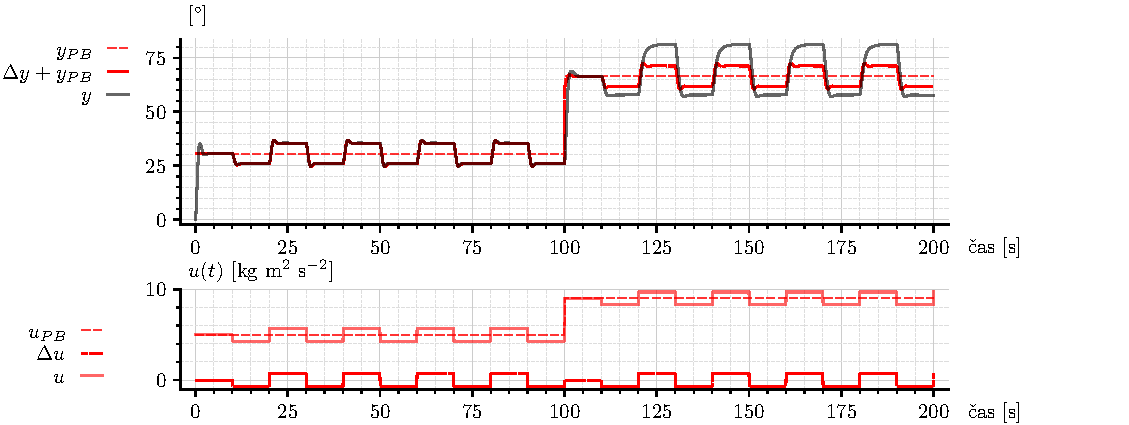
\includegraphics{figsc_ar06_kyvadlo_ep1_1.pdf}
	}

    \vspace{-2mm}

	\caption{}
	\label{figsc_ar06_kyvadlo_ep1_1}


    \vspace{-2mm}

\end{figure}


V prvom pracovnom bode sa lineárny a nelineárny systém zhodujú ale v druhom už nie. Aby sa zhodoval, musel by lineárny model zmeniť (prispôsobiť) parametre.  Inými slovami, parametre modelu riadeného systému sa menia v závislosti od pracovného bodu. Preto je potrebné mať adaptívny riadiaci systém\ldots













\subsection{Návrh adaptívneho riadiaceho systému}


\subsubsection{Model riadeného systému}

Model riadeného systému je v tvare
\begin{equation}
       \frac{y(s)}{u(s)} = k_p \frac{Z_p(s)}{R_p(s)}
\end{equation}
kde $k_p > 0$, $Z_p(s) = 1$ a $R_p(s) = s^2 + a_1s + a_0$, pričom parametre $a_1$ a $a_0$ sú neznáme (prípadne sa menia spĺňajúc však vlastnosti kvázistacionárnosti). Rád systému (stupeň polynómu $R_p(s)$) je $n = 2$ a relatívny stupeň uvedenej prenosovej funkcie je $n^* = 2$.




\subsubsection{Cieľ riadenia a referenčný model}

Cieľom riadenia je aby výstupná veličina riadeného systému sledovala výstupnú veličinu referenčného modelu, ktorý je daný prenodovou funkciou v tvare
\begin{equation}
       W_m(s) = \frac{y_m(s)}{r(s)} = k_m \frac{Z_m(s)}{R_m(s)}
\end{equation}
kde $k_m = 2$, $Z_m(s) = 1$ a $R_m(s) = s^2 + 3s + 2$. Relatívny stupeň referenčného modelu sa zhoduje s relatívnym stupňom riadeného systému.

Inými slovami, cieľom riadenia je aby sa uzavretý regulačný obvod (spojenie riadiaceho a riadeného systému) zhodoval (z hľadiska ich výstupných veličín) s~referenčným modelom.




\subsubsection{Podmienky zhody}

Keďže navrhujeme klasickú schému MRAC, v prvom rade je potrebné ukázať, že existujú podmienky zhody medzi referenčným modelom a uzavretým regulačným obvodom. Teda ukázať, že existuje riešenie MRC problému (pre tento daný konkrétny prípad).

Všeobecný tvar zákona riadenia, ktorý rieši MRC problém je
\begin{equation} \label{generalControlLaw_03}
    u(t) =
    \left[{\Theta_1^\star}^\naT \frac{\alpha(s)}{\Lambda(s)}\right] u(t)
    + \left[{\Theta_2^\star}^\naT \frac{\alpha(s)}{\Lambda(s)}\right] y(t)
    + \Theta_3^\star y(t) + \Theta_4^\star r(t)
\end{equation}
kde $\alpha(s)$ je vektor obsahujúci mocniny $s$, $\alpha(s) = \begin{bmatrix} s^{n-2}, \ldots,s, 1 \end{bmatrix}^\naT$ ak $n\geq 2$, inak $\alpha(s) = 0$. Vektory $\Theta_1^\star \in \mathbb{R}^{n-1}$, $\Theta_2^\star \in \mathbb{R}^{n-1}$ a skaláry $\Theta_3^\star \in \mathbb{R}^1$, $\Theta_4^\star \in \mathbb{R}^1$ sú konštantné parametre zákona riadenia, ktorých hodnoty hľadáme.  $\Lambda(s)$ je ľubovolný monický Hurwitzov polynóm stupňa $n-1$ obsahujúci $Z_m(s)$ ako faktor
\begin{equation}
	\Lambda(s) = \Lambda_0(s) Z_m(s)
\end{equation}
a teda aj $\Lambda_0(s)$ je ľubovolný monický Hurwitzov polynóm zodpovedajúceho stupňa.


Prenosová funkcia uzavretého regulačného obvodu má následne tvar
\begin{equation}
	y
	=
	\frac{
		k_p
		Z_p
		\Theta_4^\star
		\Lambda^2
		}{
		\Lambda
		\left(
			R_p
			\left(
				\Lambda - {\Theta_1^\star}^\naT	\alpha(s)
			\right)
			-
			k_p
			Z_p
			\left(
				{\Theta_2^\star}^\naT	\alpha(s)
				+
				\Theta_3^\star \Lambda
			\right)
		\right)}
	r
\end{equation}
Potom ak platí (podmienky zhody)
\begin{subequations} \label{prezpodmzhod}
	\begin{align}
		\Theta_4^\star &= \frac{k_m}{k_p} \label{idealTheta4_03a} \\
		\Lambda &= \Lambda_0 Z_m \label{lambda_03a} \\
		R_p
		\left(
			\Lambda - {\Theta_1^\star}^\naT \alpha(s)
		\right)
		-
		k_p
		Z_p
		\left(
			{\Theta_2^\star}^\naT \alpha(s)
			+
			\Theta_3^\star \Lambda
		\right)
	    &=
	    Z_p
	    \Lambda_0
	    R_m
	\end{align}
\end{subequations}
tak uzavretý regulačný obvod a referenčný model sa zhodujú.

Je možné ukázať\footnote{Ale to tu ani náhodou robiť nebudeme\ldots}, že uvedené podmienky zhody \eqref{prezpodmzhod} majú riešenie práve vtedy ak sú splnené podmienky už doteraz uvedené a k tomu musí platiť, že $Z_p(s)$ a $Z_m(s)$ sú monické a Hurwitzove polynómy (riadený systém a RM musia mať „stabilné nuly“) a relatívny stupeň RM je rovnaký ako relatívny stupeň riadeného systému. Uvedené je splnené a preto existujú také ideálne parametre zákona riadenia ($\Theta_1^\star$, $\Theta_2^\star$, $\Theta_3^\star$ a $\Theta_4^\star$), ktoré spĺňajú cieľ riadenia.

Keďže tieto hodnoty existujú, má význam ich hľadať. Má význam ich identifikovať. Má význam ich priebežne identifikovať. Má význam adaptovať parametre riadiaceho systému.

Ak by sme nevedeli, či je vôbec možná zhoda medzi URO a RM, potom by sme nevedeli, či vôbec môže byť adaptácia (priebežná identifikácia, strojové učenie atď., atď.) úspešná.










\subsubsection{Otázka relatívneho stupňa riadeného systému}

Vzhľadom na fakt, že $n^* = 2$, v ďalšom sa bude využívať postup návrhu MRAC, ktorý je známy pod názvom \emph{metóda doplnenej (adaptačnej) odchýlky}. Táto metóda si vyžaduje voľbu istého polynómu $L(s)$ takého, ktorý zabezpečí, že prenosová funkcia $W_m(s)L(s)$ je striktne pozitívne reálna (SPR).

V prvom rade je potrebné zvoliť stupeň polynómu $L(s)$.

Prenosová funkcia $W_m(s)$ má relatívny stupeň $n_m^* = 2$. Aby nejaká prenosová funkcia vôbec mohla byť striktne pozitívne reálna, nemôže mať relatívny stupeň vyšší ako $1$. Voľbou stupňa $L(s)$ môžme zvoliť relatívny stupeň $W_m(s)L(s)$.

Ak bude $L(s) = s + \rho$, kde $\rho$ je nejaké reálne číslo, potom relatívny stupeň $W_m(s)L(s)$ je $1$.

Mimochodom, tiež vieme, že sa zaoberáme identitou, takou, že $L(s)L^{-1}(s) = 1$. Potrebujeme teda „pracovať“ aj s prevrátenou hodnotou polynómu $L(s)$ (potrebujeme „ďeliť polynómom“) a teda v tomto prípade musí platiť, že $\rho > 0$.

Podmienky SPR pre $W_m(s)L(s)$ sú v tomto prípade formálne splnené (viď literatúra/učebný text) okrem jednej, z ktorej plynie konkrétna voľba hodnoty parametra $\rho$, a to, že $\Re \left\{ W_m(j\omega)L(j\omega) \right\} \geq 0$ pre všetky reálne $\omega$.

V tomto prípade
\begin{align}
    W_m(j\omega)L(j\omega) = \frac{ \left( 2\rho + j2\omega \right) \left( \left( 2 - \omega^2 \right) - j3\omega \right)   }%
                                  { \left( 2 - \omega^2 \right)^2 + \left( 3\omega \right)^2 }
\end{align}
a teda
\begin{align}
    \Re \left\{ W_m(j\omega)L(j\omega) \right\} = 4\rho - 2\rho\omega^2 + 6\omega^2
\end{align}
keďže $4\rho>0$ potom musí platiť $2\rho\omega^2 \leq 6\omega^2$ a teda $0 < \rho \leq 3$.
Zvoľme
\begin{equation}
      \rho = 3
\end{equation}





\subsubsection{Zákon riadenia}

Zákon riadenia (s adaptovanými parametrami) bude mať v tomto prípade tvar
\begin{equation}
	u(t) = \Theta_1(t) \left[ \frac{1}{(s + \lambda)} \right] u(t) + \Theta_2(t) \left[ \frac{1}{(s + \lambda)} \right] y(t) + \Theta_3(t) y(t) + \Theta_4(t) r(t)
\end{equation}




\paragraph{Voľba dynamiky pomocných fitrov}

Zákon riadenia využíva pomocné filtre, ktorých dynamika je daná voľbou polynómu $\Lambda(s)$. V tomto prípade $\Lambda(s) = s + \lambda$.

Polynóm $\Lambda(s)$ má súvislosť s pojmom pozorovateľ stavu, ktorý sa používa pri zostavení zákona riadenia v prípade MRC problému vo všeobecnosti. Kým teda polynóm $\Lambda(s)$ musí spĺňať isté formálne podmienky, ktoré sme už uviedli, mal by zohľadňovať aj súvislosť s pozorovateľom stavu.

Dynamika pozorovateľa stavu by vo väčšine prípadov mala byť rýchlejšia ako ostatné dymaniky vystupujúce v systéme ako celku. V tomto prípade však viac-menej nepoznáme napríklad dynamiku riadeného systému. Poznám len dynamiku referenčného modelu. Preto zabezpečme, aby polynóm $\Lambda(s)$ určoval rýchlejšiu dynamiku oproti referenčnému modelu.

Frekvenčné pásmo referenčného modelu odráža parameter $a_{0m}$. Zvoľme preto
\begin{align}
    \lambda = 10 \cdot a_{0m}
\end{align}



\paragraph{Implementácia zákona riadenia}

Ide o lineárny zákon riadenia. Preto je ho možné zapísať v tvare
\begin{align}
    u(t) = \Theta^\naT(t) \omega(t)
\end{align}
kde $\omega(t)$ je tzv. signálny vektor a $\Theta(t)$ je vektor parametrov zákona riadenia. Ku každnému signálu vo vektore $\omega(t)$ jednoznačne prislúcha parameter (prvok) z vektrora $\Theta(t)$.

\bigskip

\centerline{Je potrebné zostaviť signálny vektor $\omega(t)$.}

\bigskip

\noindent
Prvý člen v (teoretickom) zákone riadenia je možné zapísať ako prenosovú funkciu (zaviedli sme jej fiktívny výstup $y_{\nu_1}$ a dovoľujeme si nepísať všetky formálne detaily/predpoklady ako $y_{\nu_1}${\color{Gray}$(s)$} a podobne)
\begin{equation}
	y_{\nu_1} =   \frac{\Theta_1}{(s + \lambda)} u
\end{equation}
To je možné zapísať opisom v stavovom priestore:
\begin{subequations}
    \begin{align}
         \dot \nu_1 &= -\lambda \nu_1 + u \\
         y_{\nu_1} &= \Theta_1 \nu_1
    \end{align}
\end{subequations}
kde sme zaviedli stavovú veličinu (vo všeobecnosti stavový vektor) $\nu_1$. Prvý člen zákona riadenia teda nahrádza výraz
\begin{align}
     \Theta_1 \nu_1
\end{align}
Analogicky, druhý člen zákona riadenia nahrádza výraz $\Theta_2 \nu_2$ pričom $\dot \nu_2 = -\lambda \nu_2 + y$.

Signálny vektor $\omega(t)$ teraz môžme zostaviť napr. ako
\begin{align}
    \omega(t) =
    \begin{bmatrix}
        y(t) \\ \nu_1(t) \\ \nu_2(t) \\ r(t)
    \end{bmatrix}
\end{align}
Tejto voľbe potom prislúcha vektor parametrov $\Theta(t)$ v tvare
\begin{align}
    \Theta(t) =
    \begin{bmatrix}
        \Theta_3(t) \\ \Theta_1(t) \\ \Theta_2(t) \\ \Theta_4(t)
    \end{bmatrix}
\end{align}

Jednotlivé signály v signálnom vektore $\omega(t)$ sú buď priamo dostupné ($y(t)$, $r(t)$), alebo je ich potrebné vyrobiť pomocnými filtrami ($\nu_1(t)$, $\nu_2(t)$).








\subsubsection{Zákon adaptácie}


Zákon adaptácie je v tomto prípade v tvare
\begin{equation}
	\dot \Theta(t) = - \texttt{sign}\left(\frac{1}{\Theta_4^\star}\right) \Gamma \ e_1(t) \  \omega_f(t)
\end{equation}
kde vektor $\omega_f(t)$ má zložky $\omega_f(t) = \begin{bmatrix} y_f(t) & {\nu_1}_f(t) & {\nu_2}_f(t) & r_f(t) \end{bmatrix}^\naT$. Tieto signály získame jednoducho prechodom pôvodných signálov $y(t)$, $\nu_1(t)$, $\nu_2(t)$ a $r(t)$ cez filtre s prenosovou funkciou v tvare $\frac{1}{s+\rho}$.

Matica $\Gamma > 0$ má rozmer daný dĺžkou vektora $\omega_f(t)$, čo je v tomto prípade 4, teda matica $\Gamma$ má rozmer $4 \times 4$. Bude sa uvažovať diagonálna matica $\Gamma$ s kladnými číslami na diagonále (spĺňa kladnú definitnosť).

Signál $e_1(t)$ je v tomto prípade signál doplnenej adaptačnej odchýlky. Je možné ukázať, že tento signál je výsledkom rovnice
\begin{equation} \label{rovdopadaptodch}
	e_1(t) = \left(y(t) - y_m(t)\right) - \texttt{sign}\left(\frac{1}{\Theta_4^\star}\right) \left[ W_m(s) L(s) \right]  \left( \left[L(s)^{-1}\right] u(t) - \Theta^\naT(t) \omega_f(t) \right)
\end{equation}




\paragraph{Implementácia zákona adaptácie}


\subparagraph{Matica $\Gamma$}
Matica $\Gamma$ sa uvažuje, ako bolo uvedené, v tvare
\begin{equation}
    \Gamma =
    \begin{bmatrix}
        \gamma_1 & 0 & 0 & 0 \\
        0 & \gamma_2 & 0 & 0 \\
        0 & 0 & \gamma_3 & 0 \\
        0 & 0 & 0 & \gamma_4
    \end{bmatrix}
\end{equation}
s kladnými číslami $\gamma_1, \cdots, \gamma_4$.



\subparagraph{Vektor $\omega_f(t)$}

Vektor $\omega_f(t)$ je možné získať aj tak, že zostavýme MIMO systém, ktorý bude mať na vstupe signál (vektor) $\omega(t)$ a na výstupe samozrejme $\omega_f(t)$. Takýto MIMO systém je vlastne len niekoľko filtrov paralelne vedľa seba.

Vysvetlime to na príklade len dvoch signálov z vektora $\omega(t)$. Konkrétne $r(t)$ a $y(t)$. Potrebujeme spraviť napr.
\begin{equation}
    y_f(s) = \frac{1}{s+\rho} y(s)
\end{equation}
To sa dá zapísať aj ako (v stavovom priestore/opise)
\begin{equation}
    \dot y_f(t) = -\rho y_f(t) + y(t)
\end{equation}
Rovnako aj
\begin{equation}
    \dot r_f(t) = -\rho r_f(t) + r(t)
\end{equation}
Posledné dve rovnice je možné zapísať aj spolu v jednej maticovej rovnici
\begin{align}
    \begin{bmatrix}
        \dot y_f(t) \\ \dot r_f(t)
    \end{bmatrix}
    =
    \begin{bmatrix}
        -\rho & 0 \\ 0 & -\rho
    \end{bmatrix}
    \begin{bmatrix}
         y_f(t) \\  r_f(t)
    \end{bmatrix}
    +
    \begin{bmatrix}
        1 & 0 \\ 0 & 1
    \end{bmatrix}
    \begin{bmatrix}
         y(t) \\  r(t)
    \end{bmatrix}
\end{align}

Takže, ak potrebujeme „naraz“ filtrovať signálny vektor $\omega(t)$ je to možné urobiť v~zmysle:
\begin{align}
    \begin{bmatrix}
        \dot y_f(t) \\ \dot \nu_{1f}(t) \\ \dot \nu_{2f}(t) \\ \dot r_f(t)
    \end{bmatrix}
    &=
    \begin{bmatrix}
        -\rho & 0 & 0 & 0 \\
        0 & -\rho & 0 & 0 \\
        0 & 0 & -\rho & 0 \\
        0 & 0 & 0 & -\rho
    \end{bmatrix}
    \begin{bmatrix}
        y_f(t) \\ \nu_{1f}(t) \\ \nu_{2f}(t) \\ r_f(t)
    \end{bmatrix}
    +
    \begin{bmatrix}
        1 & 0 & 0 & 0 \\
        0 & 1 & 0 & 0 \\
        0 & 0 & 1 & 0 \\
        0 & 0 & 0 & 1
    \end{bmatrix}
    \begin{bmatrix}
        y(t) \\ {\nu_1}(t) \\ {\nu_2}(t) \\ r(t)
    \end{bmatrix}
    \\
    \omega_f(t)
    &=
    \begin{bmatrix}
        1 & 0 & 0 & 0 \\
        0 & 1 & 0 & 0 \\
        0 & 0 & 1 & 0 \\
        0 & 0 & 0 & 1
    \end{bmatrix}
    \begin{bmatrix}
        y_f(t) \\ \nu_{1f}(t) \\ \nu_{2f}(t) \\ r_f(t)
    \end{bmatrix}
\end{align}

Mimochodom, rovnako sa dá postupovať aj keď je $L(s)$ vyššieho ako  1. stupňa (čo možno nie je z uvedeného očividné, ale dá sa).




\subparagraph{Signál $\left( \left[L(s)^{-1}\right] u(t) - \Theta^\naT(t) \omega_f(t) \right)$}

Tento signál je potrebný pre doplnenie adaptačnej odchýlky v~rovnici \eqref{rovdopadaptodch}.

Označme ho $u_{W_mL}(t)$.

Má dve zložky. Jenou zložkou je $\Theta^\naT(t) \omega_f(t)$. Oba prvky sú k dispozícii, takže túto zložku máme k dispozícii.

Druhou zložkou je signál $\left[L(s)^{-1}\right] u(t) = u_f(s) = \frac{1}{s+\rho} u(s)$ a teda toto je možné zrealizovať ako
\begin{equation}
    \dot u_f(t) = -\rho u_f(t) + u(t)
\end{equation}
Formálne teda signál $u_{W_mL}(t)$ je
\begin{equation}
    u_{W_mL}(t) = u_f(t) + \Theta^\naT(t) \omega_f(t)
\end{equation}





\subparagraph{Signál dopĺňajúci adaptačnú odchýlku}

Tento signál v~rovnici \eqref{rovdopadaptodch} teraz môžme písať v tvare
\begin{equation}
	e_d(t) =  \texttt{sign}\left(\frac{1}{\Theta_4^\star}\right) \left[ W_m(s) L(s) \right]  u_{W_mL}(t)
\end{equation}

V prvom rade, znamienko $\texttt{sign}\left(\frac{1}{\Theta_4^\star}\right)$ je známe. Prenosová funkcia $W_m(s) L(s)$ je v tomto prípade v tvare
\begin{align}
    W_m(s) L(s) = \frac{ k_m s + k_m \rho }{ s^2 + a_{1m}s + a_{0m} }
\end{align}
Teda signál $e_d(t)$ je možné získať sústavou diferenciálnych rovníc v tvare
\begin{align}
	\dot x_{W_mL}(t)
	&=
	\begin{bmatrix}
    	0 & 1 \\
    	- a_{0m} & - a_{1m}
  	\end{bmatrix}
    x_{W_mL}(t)
    +
    \begin{bmatrix}
    	  0 \\
		  1
 	\end{bmatrix}
    u_{W_mL}(t)
    \\
    e_d(t)
    &=
    \texttt{sign}\left(\frac{1}{\Theta_4^\star}\right)
    \begin{bmatrix}
        k_m \rho & k_m \\
    \end{bmatrix}
    x_{W_mL}(t)
\end{align}




\subparagraph{Výsledná adaptačná odchýlka}

Výslednú (doplnenú) adaptačnú odchýlku je teraz možné písať ako
\begin{equation}
	e_1(t) = y(t) - y_m(t) - e_d(t)
\end{equation}















\subsubsection{Vytvorenie predstavy o nastavení rýchlosti adaptácie}

Majme nejakú predstavu o riadenom systéme. V realite azda vždy budeme mať. Tu sa to teraz myslí, tak, že máme aspoň nejakú predstavu o parametroch lineárneho modelu skutočného riadeného systému (nelineárneho kyvadla). Použime tie isté parametre, aké sme už použili pre ilustračné účely, teda hodnoty parametrov \eqref{parsysdemo}. Zostavme simulačnú schému MRAC vstupno-výstupného avšak s tým, že riadeným systémom je priamo tento lineárny model. Umožní nám to vytvoriť si predstavu o tom, ako zvoliť maticu $\Gamma$ tak, aby rýchlosť adaptácie bola prijateľná.

Pre začiatok, uvažujme všetky váhy (prvky na diagonále) v $\Gamma$ rovnaké, o veľkosti „aby sa niečo dialo“. V tomto prípade je to
\begin{equation*}
    \Gamma = \texttt{diag}
    \left(
    \begin{bmatrix}
        1000 & 1000 & 1000 & 1000
    \end{bmatrix}
    \right)
\end{equation*}
a zároveň uvažujeme harmonický signál s relatívne nízkou frekvenciou pre najjednoduchší možný prípad čo sa „obtiažnosti adaptácie“ týka. Výsledok je na obr.~\ref{figsc_ar06_kyvadlo_ep2_1}.



\begin{figure}[!t]
	\centering

    \vspace{-3mm}

	\makebox[\textwidth][c]{%
	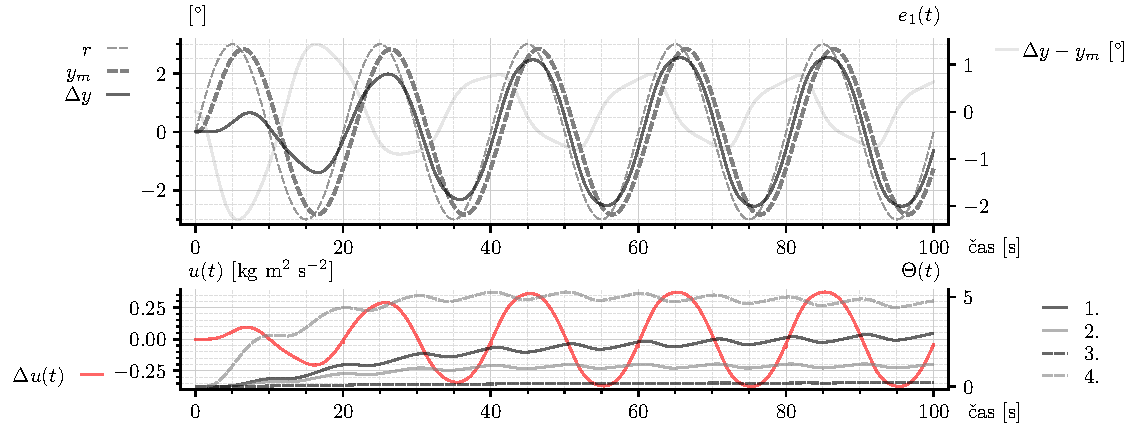
\includegraphics{figsc_ar06_kyvadlo_ep2_1.pdf}
	}

    \vspace{-2mm}

	\caption{}
	\label{figsc_ar06_kyvadlo_ep2_1}


    \vspace{-2mm}

\end{figure}













\begin{figure}[!b]
	\centering

    \vspace{-3mm}

	\makebox[\textwidth][c]{%
	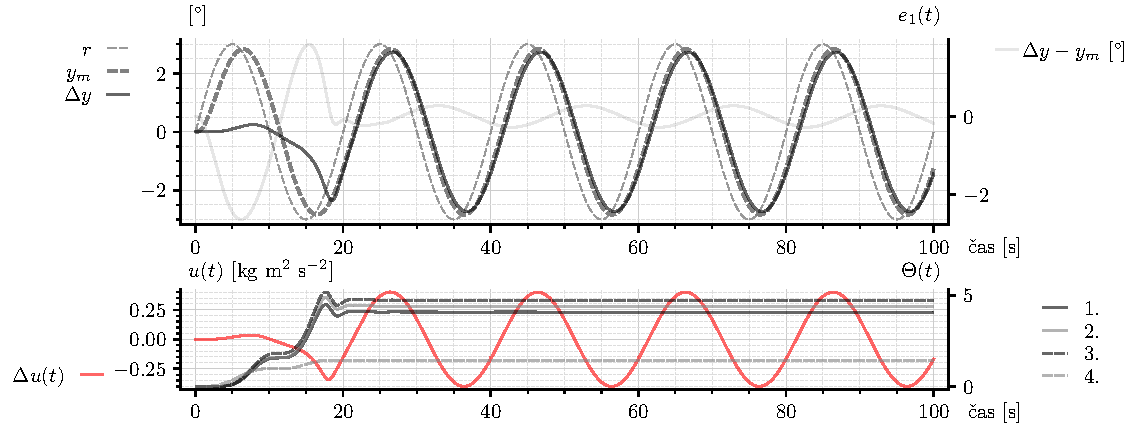
\includegraphics{figsc_ar06_kyvadlo_ep2_2.pdf}
	}

    \vspace{-2mm}

	\caption{}
	\label{figsc_ar06_kyvadlo_ep2_2}


    \vspace{-2mm}

\end{figure}






Je zrejmé, že je potrebné ladiť $\Gamma$ tak, aby rýchlosť zmeny adaptovaných parametrov bola (aspoň na začiatku) čo najviac rovnaká. Po chvíli experimentovania sa dá dospieť k voľbe
\begin{equation*}
    \Gamma = \texttt{diag}
    \left(
    \begin{bmatrix}
        7290 & 12150 & 121500 & 270
    \end{bmatrix}
    \right)
\end{equation*}
a výsledok je na obr.~\ref{figsc_ar06_kyvadlo_ep2_2}. Toto je už uspokojivý priebeh adaptovaných parametrov čo sa rýchlosti adaptácie týka.










Fungovalo by toto nastavenie aj pre iný priebeh referenčného signálu? Viď výsledok na obr.~\ref{figsc_ar06_kyvadlo_ep2_3}. Kupodivu fungovalo.






\begin{figure}[!t]
	\centering

    \vspace{-3mm}

	\makebox[\textwidth][c]{%
	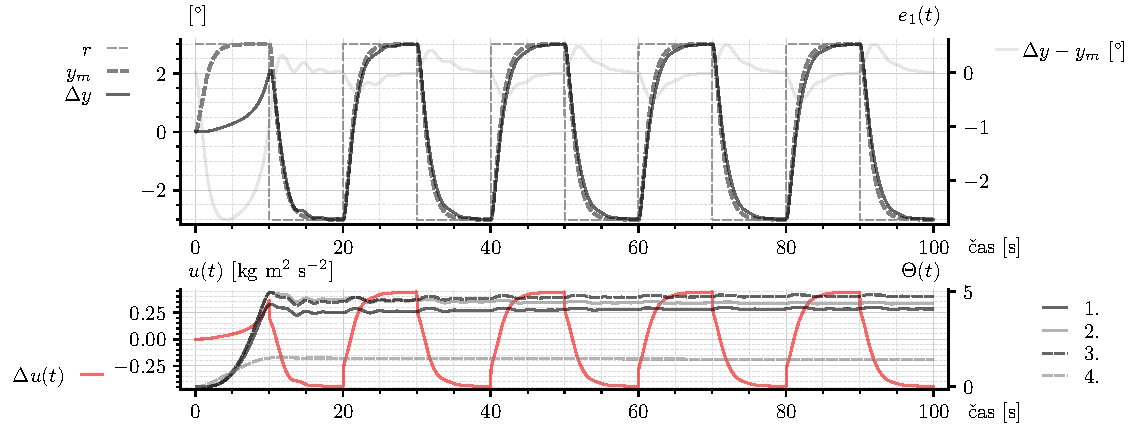
\includegraphics{figsc_ar06_kyvadlo_ep2_3.pdf}
	}

    \vspace{-2mm}

	\caption{}
	\label{figsc_ar06_kyvadlo_ep2_3}


    \vspace{-2mm}

\end{figure}














\subsection{Nasadenie na uvažovaný nelineárny systém}


Fungovalo by toto riadenie aj keby bolo nasadené na nelineárny systém? Teda priamo na nelineárne kyvadlo. Vyskúšajme - viď obr.~\ref{figsc_ar06_kyvadlo_ep3_1}. Fungovalo\ldots Aj pre obdĺžnikový referenčný signál? Fungovalo\ldots viď obr.~\ref{figsc_ar06_kyvadlo_ep3_2}.




\begin{figure}[!b]
	\centering

    \vspace{-3mm}

	\makebox[\textwidth][c]{%
	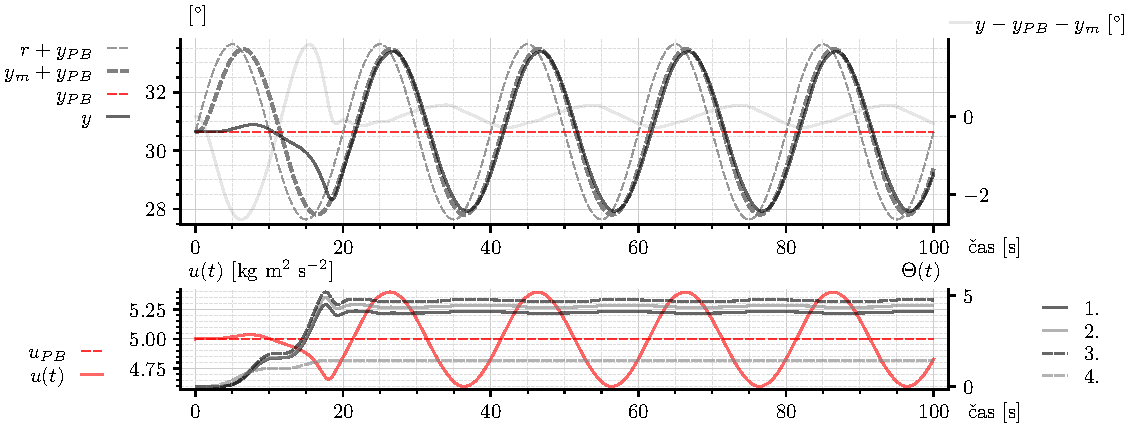
\includegraphics{figsc_ar06_kyvadlo_ep3_1.pdf}
	}

    \vspace{-2mm}

	\caption{}
	\label{figsc_ar06_kyvadlo_ep3_1}


    \vspace{-2mm}

\end{figure}










\begin{figure}[!t]
	\centering

    \vspace{-3mm}

	\makebox[\textwidth][c]{%
	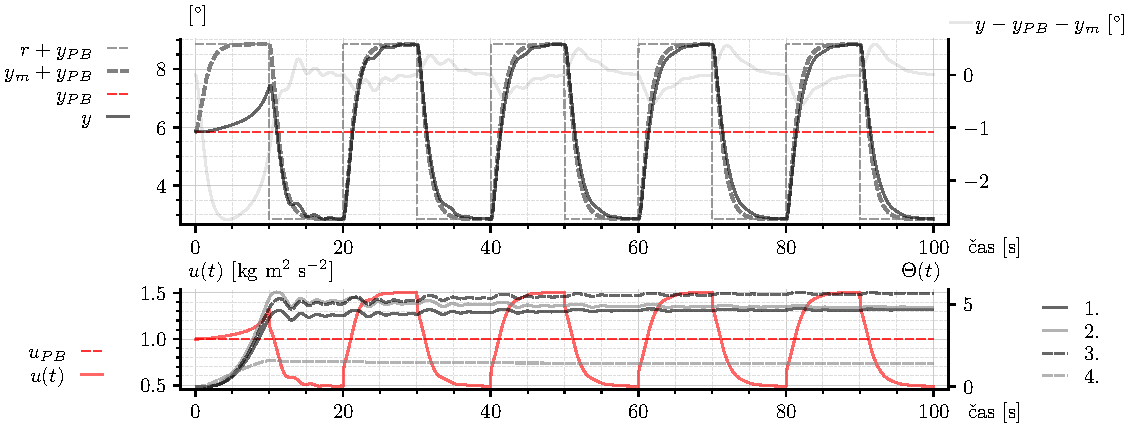
\includegraphics{figsc_ar06_kyvadlo_ep3_2.pdf}
	}

    \vspace{-2mm}

	\caption{}
	\label{figsc_ar06_kyvadlo_ep3_2}


    \vspace{-2mm}

\end{figure}






Vyskúšajme teraz simuláciu, kde v čase 100 zmeníme pracovný bod na hodnotu $u_{PB} = 6$ (z pôvodnej hodnoty $u_{PB} = 5$), necháme ustáliť sa kyvadlo v novom pracovno bode a potom budeme chcieť aby výstup sledoval RM tak ako v predch. pracovnom bode. Avšak, v čase 100 zároveň vypneme adaptáciu. Teda necháme adaptované parametre na hodnote, na ktorej boli v čase 100. Výsledok je na obr.~\ref{figsc_ar06_kyvadlo_ep3_3}.



Je zrejmé, že ak bol riadiaci systém naadaptovaný v jednom pracovnom bode, v~inom už nespĺňa cieľ radenia.



Zapnime preto adaptáciu aj po prechode do nevého pracovného bodu. Výsledok je na obr.~\ref{figsc_ar06_kyvadlo_ep3_4}. Parametre riadiaceho systému sa adaptovali na nový pracovný bod. Môžme spraviť aj zmenu na iný pracovný bod, napríklad na  $u_{PB} = 9$. Výsledok je na obr.~\ref{figsc_ar06_kyvadlo_ep3_5}. Prípadne ešte extrémnejšiu zmenu z $u_{PB} = 1$ na  $u_{PB} = 9$. Výsledok je na obr.~\ref{figsc_ar06_kyvadlo_ep3_6}.



\begin{figure}[!t]
	\centering

    \vspace{-3mm}

	\makebox[\textwidth][c]{%
	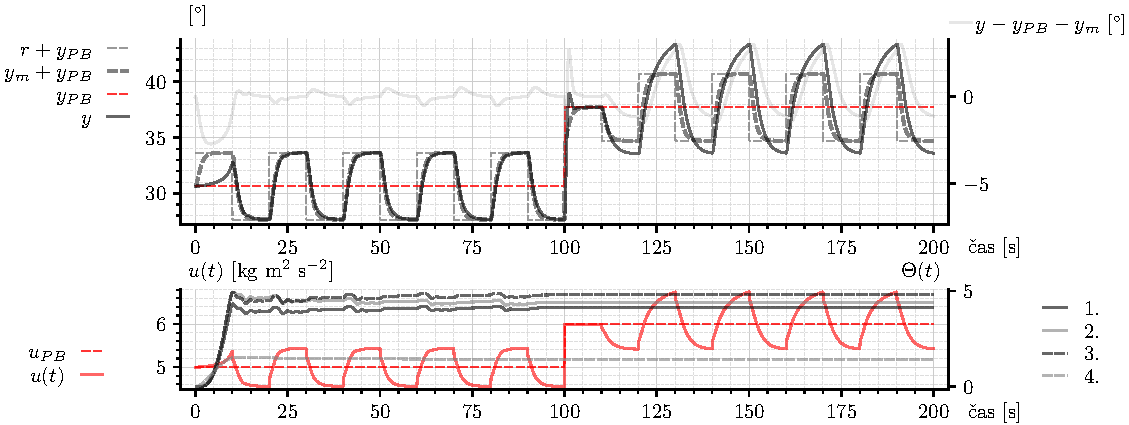
\includegraphics{figsc_ar06_kyvadlo_ep3_3.pdf}
	}

    \vspace{-2mm}

	\caption{}
	\label{figsc_ar06_kyvadlo_ep3_3}


    \vspace{-2mm}

\end{figure}








\begin{figure}[!t]
	\centering

    \vspace{-3mm}

	\makebox[\textwidth][c]{%
	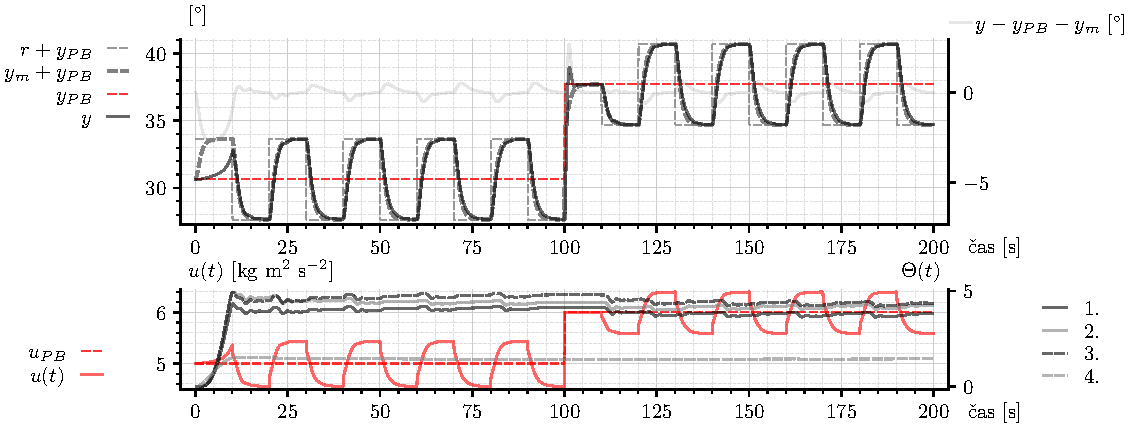
\includegraphics{figsc_ar06_kyvadlo_ep3_4.pdf}
	}

    \vspace{-2mm}

	\caption{}
	\label{figsc_ar06_kyvadlo_ep3_4}


    \vspace{-2mm}

\end{figure}








\begin{figure}[!t]
	\centering

    \vspace{-3mm}

	\makebox[\textwidth][c]{%
	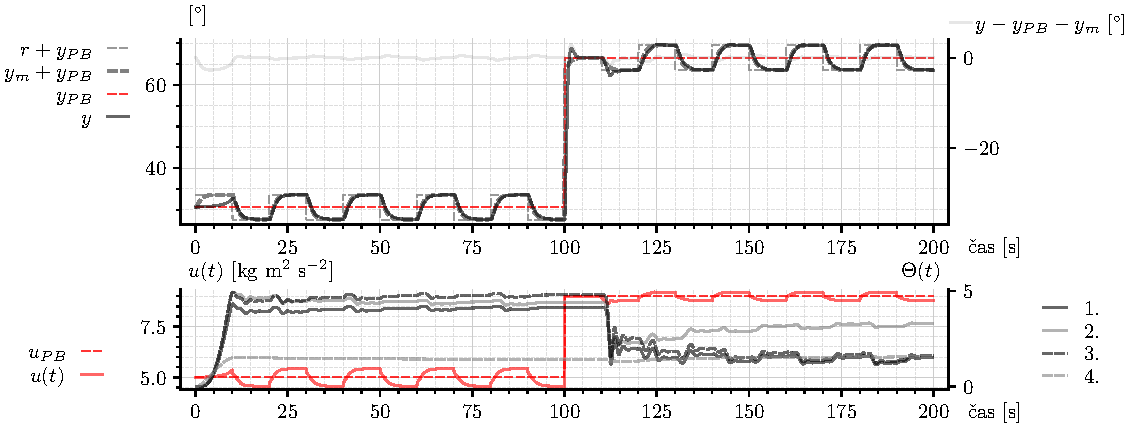
\includegraphics{figsc_ar06_kyvadlo_ep3_5.pdf}
	}

    \vspace{-2mm}

	\caption{}
	\label{figsc_ar06_kyvadlo_ep3_5}


    \vspace{-2mm}

\end{figure}








\begin{figure}[!t]
	\centering

    \vspace{-3mm}

	\makebox[\textwidth][c]{%
	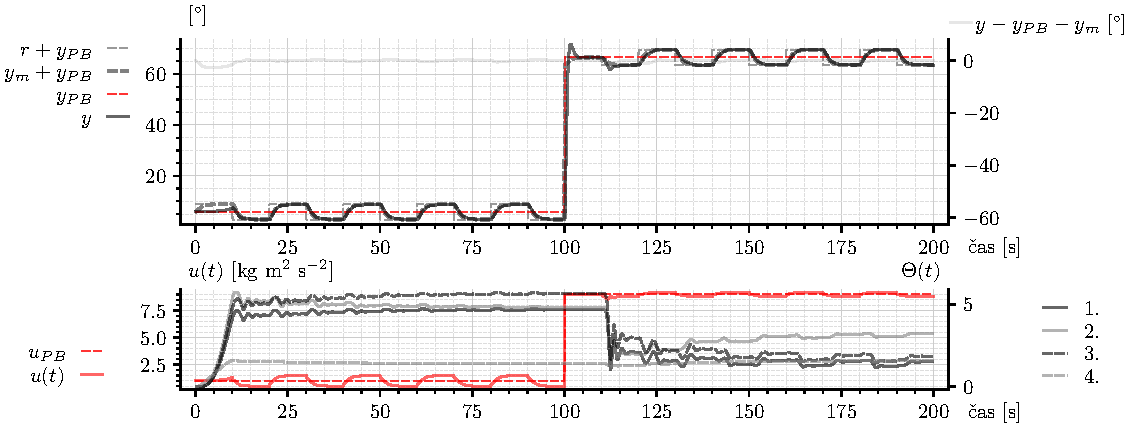
\includegraphics{figsc_ar06_kyvadlo_ep3_6.pdf}
	}

    \vspace{-2mm}

	\caption{}
	\label{figsc_ar06_kyvadlo_ep3_6}


    \vspace{-2mm}

\end{figure}




















% \clearpage

\section{Otázky a úlohy}





\begin{enumerate}[leftmargin=0pt, labelsep=4mm, itemsep=0pt]



    \item Je daný model systému
    \begin{align*}
        \dot{x}_1(t) &= x_2(t) \\
        \dot{x}_2(t) &= -a_1 x_2(t) - a_0 x_1(t) + b_0 u(t) \\
        y(t) & = x_1(t)
    \end{align*}
    kde $a_0, a_1, b_0 > 0$ sú neznáme parametre systému, $u(t)$ je vstup, $y(t)$ je výstup a~$x_1(t)$, $x_2(t)$ sú stavové veličiny systému. Tiež je daný referenčný model v tvare
    \begin{align*}
        \begin{bmatrix} \dot{x}_{1m}(t) \\ \dot{x}_{2m}(t) \end{bmatrix}
        &=
        \begin{bmatrix} 0 & 1 \\ -a_{0m} & -a_{1m} \end{bmatrix}
        \begin{bmatrix} x_{1m}(t)  \\ x_{2m}(t) \end{bmatrix}
        +
        \begin{bmatrix} 0  \\  b_{0m} \end{bmatrix}
        r(t) \\
        y_m(t) &= \begin{bmatrix} 1 & 0 \end{bmatrix}
        \begin{bmatrix} x_{1m}(t) \\ x_{2m}(t) \end{bmatrix}
    \end{align*}
    kde $a_{0m}, a_{1m}, b_{0m} > 0$ sú známe parametre referenčného modelu, $r(t)$ je referenčný signál, $y_m(t)$ je výstup a~$x_{1m}(t)$, $x_{2m}(t)$ sú stavové veličiny referenčného modelu.
    \begin{enumerate}[leftmargin=0pt, labelsep=4mm, itemsep=0pt]
        \item Napíšte model systému v~tvare prenosovej funkcie \label{odvodtePrenosFcn}
        \begin{equation*}
            \frac{y(s)}{u(s)} = k_p \frac{Z_p(s)}{R_p(s)}
        \end{equation*}
        kde $Z_p(s)$ je monický, hurwitzov polynóm stupňa $m$, $R_p(s)$ je monický polynóm stupňa $n$ a~$k_p$~je vysokofrekvenčné zosilnenie sústavy. Napíšte referenčný model v~tvare prenosovej funkcie
        \begin{equation*}
            \frac{y_m(s)}{r(s)} = W_m(s) = k_m \frac{Z_m(s)}{R_m(s)}
        \end{equation*}
        kde $k_m$ je vysokofrekvenčné zosilnenie referenčného modelu, polynóm $Z_m(s)$ je monický Hurwitzov polynóm stupňa $m_m$, $R_m(s)$ monický Hurwitzov polynóm stupňa $n_m$.

        \item Cieľom riadenia je $y = y_m$. Navrhnite ideálny zákon riadenia v~tvare
        \begin{equation*}
            u = {\Theta_1^\star}^\naT \frac{\alpha(s)}{\Lambda(s)} u + {\Theta_2^\star}^\naT \frac{\alpha(s)}{\Lambda(s)} y + \Theta_3^\star y + \Theta_4^\star r
        \end{equation*}
        kde $\alpha(s)$ je vektor obsahujúci mocniny $s$, $\alpha(s) = \begin{bmatrix} s^{n-2}, \ldots,s, 1 \end{bmatrix}^{\mathsf{T}}$ ak $n\geq 2$, inak $\alpha(s) = 0$. Vektory $\Theta_1^\star, \Theta_2^\star \in \mathbb{R}^{n-1}$ a  skaláry $\Theta_3^\star, \Theta_4^\star \in \mathbb{R}^1$ sú konštantné parametre zákona riadenia, ktorých hodnoty hľadáme.  $\Lambda(s)$ je ľubovolný monický Hurwitzov polynóm stupňa $n-1$ obsahujúci $Z_m(s)$ ako faktor
        \begin{equation*}
            \Lambda(s) = \Lambda_0(s) Z_m(s)
        \end{equation*}
        a teda aj $\Lambda_0(s)$ je ľubovolný monický Hurwitzov polynóm zodpovedajúceho stupňa.
    \end{enumerate}



    % \bigskip

    \item Odvoďte podmienky zhody pre MRAC vstupno-výstupný

    % \medskip

    \item Odvoďte podmienky zhody uzavretého regulačného obvodu a referenčného modelu.

        \begin{tabular}{@{}l @{\ } l}
            Model riadeného systému: &
            $\displaystyle \frac{y(s)}{u(s)} = k_p\frac{Z_p(s)}{R_p(s)}$
            \qquad
            \begin{tabular}{@{}l}
            rád systému $n = 2$\\
            relatívny stupeň $n^* = 1$
            \end{tabular} \vspace{1mm}\\
            Referenčný model: & $\displaystyle \frac{y_m(s)}{r(s)} = k_m\frac{Z_m(s)}{R_m(s)} $ \vspace{1mm} \\
            Zákon riadenia: & $\displaystyle u(s) = \frac{\Theta_1^\star}{\Lambda(s)} u(s) + \frac{\Theta_2^\star}{\Lambda(s)} y(s) + \Theta_3^\star y(s) + \Theta_4^\star r(s)$
        \end{tabular}









	\item Zistite či je prenosová funkcia $G(s)$ striktne pozitívne reálna (SPR).
	\begin{equation*}
		G(s) = \frac{2\,s + 1}{ (3\,s + 1) (s + 1)}
	\end{equation*}

	\item Pre aké hodnoty $a$, $b$, $c$ je prenosová funkcia $\displaystyle G(s) = \frac{as + 1}{ \left( bs + 1 \right)   \left( cs + 1 \right)   }$ striktne pozitívne reálna.


	\item Schematicky znázornite MRAC vstupno-výstupný pri $n^\star = 1$

	\item Schematicky znázornite MRAC vstupno-výstupný pri $n^\star = 2$

	\item Čo je cieľom riadenia pri návrhu adaptívneho riadiaceho systému s referenčným modelom so zákonom adaptácie navrhnutým pomocou Lyapunovovej teórie stability?


	\item Je daný model systému
	\begin{align*}
		\dot{x}_1(t) &= x_2(t) \\
		\dot{x}_2(t) &= -a_1 x_2(t) - a_0 x_1(t) + b_0 u(t) \\
		y(t) & = x_1(t)
	\end{align*}
	kde $a_0, a_1, b_0 > 0$ sú neznáme parametre systému, $u(t)$ je vstup, $y(t)$ je výstup a~$x_1(t)$, $x_2(t)$ sú stavové veličiny systému. Tiež je daný referenčný model v tvare
	\begin{align*}
		\begin{bmatrix} \dot{x}_{1m}(t) \\ \dot{x}_{2m}(t) \end{bmatrix}
        &=
		\begin{bmatrix} 0 & 1 \\ -a_{0m} & -a_{1m} \end{bmatrix}
		\begin{bmatrix} x_{1m}(t)  \\ x_{2m}(t) \end{bmatrix}
		+
		\begin{bmatrix} 0  \\  b_{0m} \end{bmatrix}
		r(t) \\
		y_m(t) &= \begin{bmatrix} 1 & 0 \end{bmatrix} \begin{bmatrix} x_{1m}(t)  \\ x_{2m}(t) \end{bmatrix}
	\end{align*}
	kde $a_{0m}, a_{1m}, b_{0m} > 0$ sú známe parametre referenčného modelu, $r(t)$ je referenčný signál, $y_m(t)$ je výstup a~$x_{1m}(t)$, $x_{2m}(t)$ sú stavové veličiny referenčného modelu.

	\begin{enumerate}[leftmargin=0pt, labelsep=4mm, itemsep=0pt]

		\item Napíšte model systému v tvare prenosovej funkcie \label{odvodtePrenosFcn2}
		\begin{equation*}
            \frac{y(s)}{u(s)} = k_p \frac{Z_p(s)}{R_p(s)}
		\end{equation*}
		kde $Z_p(s)$ je monický, hurwitzov polynóm stupňa $m$, $R_p(s)$ je monický polynóm stupňa $n$ a~$k_p$~je  vysokofrekvenčné zosilnenie sústavy. Napíšte referenčný model v~tvare prenosovej funkcie
		\begin{equation*}
			\frac{y_m(s)}{r(s)} = W_m(s) = k_m \frac{Z_m(s)}{R_m(s)}
		\end{equation*}
		kde $k_m$ je vysokofrekvenčné zosilnenie referenčného modelu, polynóm $Z_m(s)$ je monický Hurwitzov polynóm stupňa $m_m$, $R_m(s)$ monický Hurwitzov polynóm stupňa $n_m$.

		\item Ideálnym cieľom riadenia je $y = y_m$. Navrhnite ideálny zákon riadenia v~tvare
		\begin{equation*}
			u = {\Theta_1^\star}^\naT \frac{\alpha(s)}{\Lambda(s)} u + {\Theta_2^\star}^\naT \frac{\alpha(s)}{\Lambda(s)} y + \Theta_3^\star y + \Theta_4^\star r
		\end{equation*}
		kde $\alpha(s)$ je vektor obsahujúci mocniny $s$, $\alpha(s) = \begin{bmatrix} s^{n-2}, \ldots,s, 1 \end{bmatrix}^\naT$ ak $n\geq 2$, inak $\alpha(s) = 0$. Vektory $\Theta_1^\star, \Theta_2^\star \in \mathbb{R}^{n-1}$ a  skaláry $\Theta_3^\star, \Theta_4^\star \in \mathbb{R}^1$ sú konštantné parametre zákona riadenia, ktorých hodnoty hľadáme.  $\Lambda(s)$ je ľubovolný monický Hurwitzov polynóm stupňa $n-1$ obsahujúci $Z_m(s)$ ako faktor
		\begin{equation*}
			\Lambda(s) = \Lambda_0(s) Z_m(s)
		\end{equation*}
		a teda aj $\Lambda_0(s)$ je ľubovolný monický Hurwitzov polynóm zodpovedajúceho stupňa.

		\item Cieľom riadenia je $y \to y_m$ a stabilita celého riadiaceho systému. Navrhnite adaptívny riadiaci systém, pričom uvažujte model riadeného systému v~tvare prenosovej funkcie  a tiež referenčný model v tvare prenosovej funkcie z~predchádzajúceho bodu \ref{odvodtePrenosFcn2}.

	\end{enumerate}






\end{enumerate}















































\bibliography{../misc_LaTeX/Bib_KurzAR}{}
\bibliographystyle{plain}





\end{document}
